\documentclass[12pt]{article} 
\usepackage{setspace}
\usepackage{amsmath}
\usepackage{cancel}
\usepackage{algorithm}
\usepackage{graphicx}
\usepackage[noend]{algpseudocode}
\usepackage{gnuplot-lua-tikz}
\doublespacing
\begin{document}

% \begin{titlepage}

%     \title{
%         Method of Manufactured Solution Applied to SWIRL's Speed of Sound Integration
%     Technique}


%     \author{ Jeffrey Severino \\
%         University of Toledo \\
%         Toledo, OH  43606 \\
%     email: jseveri@rockets.utoledo.edu}


%     \maketitle

% \end{titlepage}

\section{Introduction}
The Method of Manufactured Solutions (MMS) is a process for generating an 
analytical solution for a code that provides the numerical solution for a 
given domain. The goal of MMS is to establish a manufactured solution that can 
be used to establish the accuracy of the code within question. For this study, 
SWIRL, a code used to calculate the radial modes within an infinitely long duct
is being validated through code verification. SWIRL accepts a given mean flow and 
uses numerical integration to obtain the speed of sound. The integration technique
is found to be the composite trapezoidal rule through asymptotic error analysis.


\section{Methods}

SWIRL is a linearized Euler equations of motion code that formulates an
eigenvalue problem calculates the 
axial wavenumber and radial mode shapes from small unsteady disturbances in a mean flow. 
The mean flow varies along the axial and tangetial directons as a function of 
radius. The flow domain can either be a circular or annular duct, with or without
acoustic liner. TSWIRL was originally written by Kousen [insert ref].

The SWIRL code requires two mean flow parameters as a function of radius, $M_x$
, and $M_{\theta}$. The speed of sound, $\widetilde{A}$ is calculated by 
integrating $M_{\theta}$ with respect to r. To verify that SWIRL is handling 
and returning the accompanying mean flow parameters, the error between the 
mean flow input and output variables are computed. Since the trapezoidal rule
is used to numerically integrate $M_{\theta}$, the discretization error and 
order of accuracy is computed. Since finite differencing schemes are to be used 
on the result of this integration, it is crucial to accompany the integration 
with methods of equal or less order of accuracy. This will be determined by 
applying another MMS on the eigenproblem which will also have an order of 
accuracy.

\subsection{Theory}

To relate the speed of sound to a given flow, the radial momentum equation
is used.  If the flow contains a swirling component,then the primitive variables 
are nonuniform through the flow, and mean flow assumptions are not valid. 
% \begin{align*}
%     \frac{\partial v_r}{\partial t} +
%     v_r \frac{\partial v_r}{\partial r} + 
%     \frac{v_{\theta}}{r} 
%     \frac{\partial v_{\theta}}{\partial \theta} -
%     \frac{v_{\theta}^2}{r} _ 
%     v_x \frac{\partial v_r}{\partial x} =
%     \frac{1}{\rho}\frac{\partial P}{\partial r}
% \end{align*}

 To account to for this, the radial momentum is simplified by assuming the 
 flow is steady, the flow has no radial component. In addition, the viscous
 and body forces are neglected.
 
 The the radial pressure derivative term is set equal to the dynamic pressure term
 and seperation of variables is applied.  

 \begin{align*}
     \frac{v_{\theta}^2}{r} = \frac{1}{\rho}\frac{\partial P}{\partial r} \\
 P = \int_{r}^{r_{max}} \frac{\rho V_{\theta}^2}{ \partial r}
 \end{align*}
 
% \[\] 

% where $\tilde{r}$ is the radius dimensional radius normalized 
% by the tip diameter $r_t = r_{max}$

% To show the work, we will start with the dimensional form of the equation and
% differentiate both sides,
% \[
% \]
% Applying separation of variables,
% \[
%     \int_{r}^{r_{max}}
%     \frac{\bar{\rho} v_{\theta}^2}{r} \partial r 
%     =-\int_{P(r)}^{P(r_{max})}\partial p
% \]

Since $\tilde{r} = r/r_{max}$,
\[r = \tilde{r}r_{max}.\]
Taking total derivatives (i.e. applying chain rule),
\[dr = d(\tilde{r}r_{max}) = d(\tilde{r})r_{max}\]
Substituting these back in and evaluating the right hand side,
\[
    \int_{\tilde{r}}^{1} \frac{\bar{\rho} v_{\theta}^2}{\tilde{r}}\partial \tilde{r} 
    =P(1)-P(\tilde{r})
\]

For reference the minimum value of $\tilde{r}$ is

\[\sigma = \frac{r_{max}}{r_{min}}\]

For the radial derivative, the definition of the speed of sound is utilized,
\[\frac{\partial A^2}{\partial r } =
\frac{\partial}{\partial r} \left( \frac{\gamma P}{\rho} \right).\]

Using the quotient rule, we can extract the definition of the speed of sound.

\begin{align*}
&= \frac{\partial P}{\partial r} \frac{\gamma \bar{\rho}}{\bar{\rho}^2} -
\left(
    \frac{\gamma P}{\bar{\rho}^2} 
\right) 
\frac{\partial \bar{\rho}}{\partial r}\\
&=  \frac{\partial P}{\partial r} \frac{\gamma }{\bar{\rho}} -
\left( \frac{A^2}{\bar{\rho}} \right) 
\frac{\partial \bar{\rho} }{\partial r}
\end{align*}

Using isentropic condition $ \partial P/A^2 = \partial \rho$, 

\begin{align*}
&= \frac{\partial P}{\partial r} \frac{\gamma }{\bar{\rho}} -
\left( \frac{1}{\bar{\rho}} \right) \frac{\partial  P }{\partial r}\\
\frac{\partial A^2}{\partial r} 
&= \frac{\partial P}{\partial r} \frac{\gamma - 1}{\bar{\rho}}  
\end{align*}

\begin{align*}
    \frac{\bar{\rho}}{\gamma -1}\frac{\partial A^2}{\partial r} &= \frac{\partial P}{\partial r} 
\end{align*}


Going back to the radial momentum equation, and rearranging the 

\begin{align*}
    \frac{\bar{\rho} v_{\theta}^2}{r} 
&=\frac{\partial P}{\partial r}\\
\frac{\cancel{
        \bar{\rho}
} v_{\theta}^2}{r} 
&=\frac{\cancel{\bar{\rho}}}{\gamma -1}\frac{\partial A^2}{\partial r}\\
    \frac{v_{\theta}^2}{r}\left(\gamma -1\right) &= \frac{\partial A^2}{\partial r}
\end{align*}
To start the nondimensionalization, we define,

\begin{align*}
    M_{\theta} &= \frac{V_{\theta}}{A} \\ 
    \widetilde{r} &= \frac{r}{r_{max}}  \\
    \widetilde{A} &= \frac{A}{A_{r,max}}  \\
    A &= \widetilde{A}{A_{r,max}} \\
    r &= \widetilde{r}{r_{max}}\\
    \frac{\partial}{\partial r} &=
    \frac{\partial \widetilde{r}}{\partial r} \frac{\partial}{\partial \widetilde{r}}\\
                                &= \frac{1}{r_{max}}\frac{\partial}{\partial \widetilde{r}}
\end{align*}
Dividing by $A$,
\begin{align*}
    \frac{M_{\theta}^2}{r}\left(\gamma - 1\right) 
&= \frac{\partial A^2}{\partial r} \frac{1}{A^2}
\end{align*}

At this point we can either find the derivative of  $\bar{A}$ or the integral of
$M_{\theta}$ with respect to r
\begin{enumerate}
    \item
\begin{align*}
\text{Integrating both sides } \int_{r}^{r_{max}}\frac{M_{\theta}}{r}\left(\gamma - 1\right){\partial r}  &=\int_{A^2(r)}^{A^2(r_{max})}\frac{1}{A^2}  {\partial A^2}\\
\int_{r}^{r_{max}}\frac{M^2_{\theta}}{r}\left(\gamma - 1\right){\partial r}  &=ln(A^2(r_{max})) - ln(A^2(r)) \\
\int_{r}^{r_{max}}\frac{M^2_{\theta}}{r}\left(\gamma - 1\right){\partial r}  &=ln\left(\frac{A^2(r_{max})}{A^2(r)}\right) 
\end{align*}

Defining non dimensional speed of sound $\tilde{A} = \frac{A(r)}{A(r_{max})}$
\begin{align*}
\int_{r}^{r_{max}}\frac{M_{\theta}}{r}\left(\gamma - 1\right){\partial r}  &=ln\left(\frac{1}{\tilde{A}^2}\right) \\
&= -2ln(\tilde{A})\\
\tilde{A}(r) &= exp\left[-\int_{r}^{r_{max}}\frac{M_{\theta}}{r}\frac{\left(\gamma - 1\right)}{2}{\partial r}\right] \\ \text{replacing r with }\tilde{r} \rightarrow \tilde{A}(r) &= exp\left[-\int_{r}^{r_{max}}\frac{M_{\theta}}{r}\frac{\left(\gamma - 1\right)}{2}{\partial r}\right]		\\
\tilde{A}(\tilde{r}) &= exp\left[\left(\frac{1 - \gamma}{2}\right)\int_{\tilde{r}}^{1}\frac{M_{\theta}}{\tilde{r}}{\partial \tilde{r}}\right]	
\end{align*}
\item Or we can differentiate
\end{enumerate}
Solving for $M_{\theta}$ ,
\begin{align*}
M_{\theta}^2 
&= \frac{\partial A^2}{\partial r} \frac{r}{A^2 \left(\gamma - 1\right)}
\end{align*}
Nondimensionalizing:

Plugging in,

\begin{align} 
    M_{\theta}^2
    \frac{\left( \gamma - 1 \right)}{\widetilde{r} r_{max}} &=
    \frac{1}{(\widetilde{A}A_{r,max})^2}\frac{A_{r,max}^2}{r_{max}}
    \frac{\partial \widetilde{A}^2}{\partial \widetilde{r}} \nonumber \\
    M_{\theta}^2     \frac{\left( \gamma - 1 \right)}{\widetilde{r} } &=
    \frac{1}{\widetilde{A}^2}
    \frac{\partial \widetilde{A}^2}{\partial \widetilde{r}} \nonumber \\
    M_{\theta} &= \sqrt{\frac{\widetilde{r}}{(\gamma-1) \widetilde{A}^2}
        \frac{\partial\widetilde{A}^2}{\partial \widetilde{r} }
    } \label{eq:Mthetabackcalculated}
\end{align}

3.1 Guidelines for Creating Manufactured Solutions states:
\begin{enumerate}
    \item  The manufactured solutions should be composed of smooth analytic 
        functions 
    \item The manufactured solutions should exercize every term in the governing
        equation that is being tested,
    \item The solution should have non trivial derivatives.  
    \item The solution derivatives should be bounded by a small constant. In this case
        this constant should prevent the function from becoming greater than 
        one.
    \item The solution should not prevent the code from running 
    \item The solution should be defined on a connected subset of two- or three-
        dimensional space to allow flexibility in chosing the domain of the PDE.
        Section 3.3.1 provides more information about this.
    \item The solution should coincide with the differential operators of the PDE.
        For example, the flux term in Fourier's law of conduction requires T to 
        be differentiable.
\end{enumerate}
With these guidelines, a function is specified for the speed of sound to conduct
a method of manufactured solutions on SWIRL's speed of sound numerical 
integration. This is checked by observing the tangential mach number 
produced from the speed of sound and comparing that to the tangential mach number
that has been analytically defined (See Equation \ref{eq:Mthetabackcalculated}).
\subsection{Procedure}

There are a few constraints and conditions that must be followed in order for the analytical 
function to have physical significance.
\begin{itemize}
    \item The mean flow and speed of sound must be real and positive. This will 
        occur is a speed of sound is chosen such that the tangential mach number
        is imaginary
    \item The derivative of the speed of sound must be positive
    \item Any bounding constants used with the mean flow should not allow the 
        total Mach number to exceed one.
    \item the speed of sound should be one at the outer radius of the cylinder
\end{itemize}

Given these constraints, $tanh(r)$ is chosen as a function since it can be
modified to meet the conditions above.

The benefit of tanh(r) is that it is bounded between one and negative one. 
\begin{itemize}
    \item As r $\rightarrow$ $\infty$ tanh(r) $\rightarrow$ 1
    \item As -r $\rightarrow$ $-\infty$ tanh(r) $\rightarrow$ -1
\end{itemize}

To test the numerical integration method,  $M_{\theta}$ is defined as a result 
of differentiating the speed of sound, $A$. This is done opposed to integrating
$M_{\theta}$. However, a function can be defined for $M_{\theta}$, which can 
then be integrated to find what $\widetilde{A}$ should be. 
Instead, the procedure of choice is to back calculate what the appropriate 
$M_{\theta}$ is for a given expression for $\widetilde{A}$.

Since it is easier to take derivatives , we will solve for $M_{\theta}$ using 
Equation \ref{eq:Mthetabackcalculated} ,

\begin{align*}
    M_{\theta} = \sqrt{ \frac{\widetilde{r}}{(\gamma -1) \widetilde{A}^2} 
    \frac{\partial \widetilde{A}^2}{\partial \widetilde{r}}}
\end{align*}

This time we define the speed of sound with the subscript $analytic$ to indicate 
that this is the analytical function of choice and has no physical relevance 
to the actual problem.

\begin{align*}
\widetilde{A}_{analytic} = \Lambda + k_1 \tanh \left( k_2 \left( \widetilde{r} - \widetilde{r}_{max} \right) \right),
\end{align*}

where, 

\begin{align*}
    \Lambda = 1 - k_1 \tanh(k_2 (1 - \widetilde{r}_{max})),
\end{align*}

When, $\widetilde{r}=\widetilde{r}_{max}$ , $\widetilde{A}_{analytic} = 1$.  
Taking the derivative with respect to $\widetilde{r}$,

\begin{align*}
    \frac{\partial \widetilde{A}_{analytic} }{\partial \widetilde{r}} &=
    \left(1 - \tanh^{2}{\left(\left(r - r_{max}\right) {k}_{2} \right)}\right) {k}_{1} {k}_{2}, \\ 
    &= \frac{ k_{1} k_{2}}{\cosh^{2}{\left(\left(r - r_{max}\right) {k}_{2} \right)}}.
\end{align*}

Now / substitute this into the expression for $M_{\theta}$ in Equation 
\ref{eq:Mthetabackcalculated},

\begin{align*}
    M_{\theta} = \sqrt{2}
    \sqrt{\frac{r {k}_{1} {k}_{2}}{\left(\kappa - 1\right) \left(\tanh{\left(\left(r - r_{max}\right) {k}_{2} \right)} {k}_{1} + \tanh{\left(\left(r_{max} - 1\right) {k}_{2} \right)} {k}_{1} + 1\right) \cosh^{2}{\left(\left(r - r_{max}\right) {k}_{2} \right)}}}
\end{align*} 

Now that the mean flow is defined, the integration method used to obtain the 
speed of sound

What happens when $r = r_{max}$?

\subsection{Calculation of Observed Order-of-Accuracy}
The numerical scheme used to perform the integration of the tangential velocity
will have a theoretical order-of-accuracy. To find the theoretical order-of-accuracy,
the discretization error must first be defined. The error, $\epsilon$, is a function of id spacing, $\Delta r$

\[ \epsilon = \epsilon(\Delta r) \]
The discretization error in the solution should be proportional to 
$\left( \Delta r \right)^{\alpha}$ where $\alpha > 0$ is the theoretical order
for the computational method.  The error for each grid is expressed as 
\[ \epsilon_{M_{\theta}}(\Delta r) = |M_{\theta,analytic}-M_{\theta,calc}|\]
where $M_{\theta,analytic}$ is the tangential mach number that is defined from the
speed of sound we also defined and the $M_{\theta,calc}$ is the result from 
SWIRL. The $\Delta r$ is to indicate that this is a discretization error for a
specific grid spacing. Applying the same concept to to the speed of sound,

If we define this error on various grid sizes and compute $\epsilon$ for
each grid, the observed order of accuracy can be estimated and compared to
the theoretical order of accuracy. For instance, if the numerical soution
is second-order accurate and the error is converging to a value, the L2 norm of
the error will decrease by a factor of 4 for every halving of the grid cell 
size. 
Since the input variables should remain unchanged (except from minor changes 
from the Akima interpolation), the error for the axial and tangential mach 
number should be zero. As for the speed of sound, since we are using an analytic
expression for the tangential mach number, we know what the theoretical result
would be from the numerical integration technique as shown above. 
Similarly we define the discretization error for the speed of sound.

\[ \epsilon_{A}(\Delta r) = |A_{analytic}-A_{calc}|\]

For a perfect answer, we expect $\epsilon$ to be zero. Since a Taylor series can 
be used to derive the numerical schemes, we know that the truncation of higher
order terms is what indicates the error we expect from using a scheme that 
is constructed with such truncated Taylor series.

%\text{H.O.T}
We expect the error at each grid point $j$ to satisfy the following,
\begin{align*}
    0 &= |A_{analytic}(r_j) - A_{calc}(r_j)| \\
    \widetilde{A}_{analytic}(r_j) &= \widetilde{A}_{calc}(r_j) +
    (\Delta r)^{\alpha} \beta(r_j)  + H.O.T
\end{align*}

where the value of $\beta(r_j)$ does not change with grid spacing, and 
$\alpha$ is the asymptotic order of accuracy of the method. It is important to
note that the numerical method recovers the original equations as the grid 
spacing approached zero. 

It is important to note that $\beta$ represents the first derivative of the 
Taylor Series

Subtracting $A_{analytic}$ from both sides gives

\begin{align*}
    A_{calc}(r_j) - A_{analytic}(r_j) &= A_{analytic}(r_j) - A_{analytic}(r_j)
    + \beta(r_j) (\Delta r)^{\alpha} \\
    \epsilon_A(r_j)(\Delta r) &= \beta(r_j) (\Delta r)^{\alpha}
\end{align*}

To estimate the order of accuracy of the accuracy, we define the global errors 
by calculating the L2 Norm of the error which is denoted as $\hat{\epsilon}_A$ 

% \begin{align*}
%     0 &=|A_{analytic}(r_j)-A_{calc}(r_j)| \\
%     A_{calc}(r_j) &= A_{analytic}(r_j) + \beta(r_j) (\Delta r)^{\alpha} + 
% \end{align*}

\begin{align*}
    \hat{\epsilon}_A = \sqrt{\frac{1}{N}\sum_{j=1}^{N} \epsilon(r_j)^2  }
\end{align*}

\begin{align*}
    \hat{\beta}_A(r_j) = \sqrt{\frac{1}{N}\sum_{j=1}^{N} \beta(r_j)^2  }
\end{align*}
As the grid density increases, $\hat{\beta}$ should asymptote to a constant 
value. Given two grid densities, $\Delta r$ and $\sigma\Delta r$, and assuming
that the leading error term is much larger than any other error term,

\begin{align*}
    \hat{\epsilon}_{grid 1} &= \hat{\epsilon}(\Delta r) = \hat{\beta}(\Delta r)^{\alpha} \\
    \hat{\epsilon}_{grid 2} &= \hat{\epsilon}(\sigma \Delta r) = \hat{\beta}(\sigma \Delta r)^{\alpha} \\
                            &= \hat{\beta}(\Delta r)^{\alpha} \sigma^{\alpha}
\end{align*}

The ratio of two errors is given by,

\begin{align*}
    \frac{\hat{\epsilon}_{grid 2}}{\hat{\epsilon}_{grid 1}} &= 
    \frac{\hat{\beta}(\Delta r )^{\alpha}}{\hat{\beta}(\Delta r )^{\alpha}} \sigma^{\alpha} \\ &= \sigma^{\alpha}
\end{align*}

Thus, $\alpha$,the asymptotic rate of convergence is computed as follows 

\begin{align*}
    \alpha = \frac{
        \ln \frac{
            \hat{\epsilon}_{grid 2}
    }{\hat{\epsilon}_{grid 1} }}
    {\ln\left( \sigma \right) }
\end{align*}

Defining  for a doubling of grid points ,

\begin{align*}
    \alpha = \frac{\ln \left( \hat{\epsilon}\left( \frac{1}{2}\Delta  r\right)
            \right) -\ln \left( \hat{\epsilon}\left( \Delta  r\right)
    \right)}{\ln \left( \frac{1}{2} \right)}
\end{align*}

\section{Results And Discussion}
% %        File: test.tex
%     Created: Sun Jul 18 12:00 PM 2021 E
% Last Change: Sun Jul 18 12:00 PM 2021 E
%


\begin{figure}
    \begin{center}
       % This file was created with tikzplotlib v0.9.12.
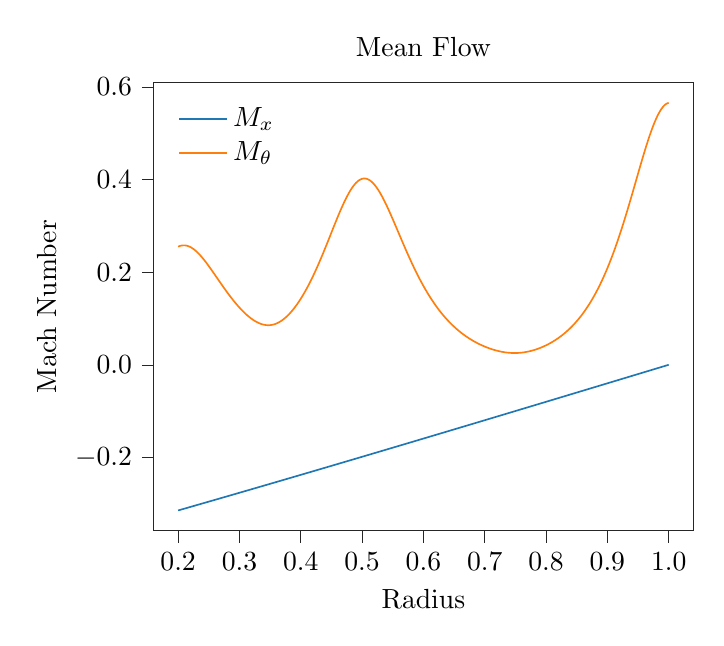
\begin{tikzpicture}

\definecolor{color0}{rgb}{0.12156862745098,0.466666666666667,0.705882352941177}
\definecolor{color1}{rgb}{1,0.498039215686275,0.0549019607843137}

\begin{axis}[
axis line style={white!15!black},
legend cell align={left},
legend style={
  fill opacity=0.8,
  draw opacity=1,
  text opacity=1,
  at={(0.03,0.97)},
  anchor=north west,
  draw=none
},
tick align=outside,
tick pos=left,
title={Mean Flow },
x grid style={white!80!black},
xlabel={Radius},
xmin=0.16, xmax=1.04,
xtick style={color=white!15!black},
xtick={0.1,0.2,0.3,0.4,0.5,0.6,0.7,0.8,0.9,1,1.1},
xticklabels={0.1,0.2,0.3,0.4,0.5,0.6,0.7,0.8,0.9,1.0,1.1},
y grid style={white!80!black},
ylabel={Mach Number},
ymin=-0.358579171685103, ymax=0.609698172253824,
ytick style={color=white!15!black},
ytick={-0.4,-0.2,0,0.2,0.4,0.6,0.8},
yticklabels={\ensuremath{-}0.4,\ensuremath{-}0.2,0.0,0.2,0.4,0.6,0.8}
]
\addplot [semithick, color0]
table {%
0.2 -0.314566565142425
0.2015625 -0.313973231598063
0.203125 -0.313379775407908
0.2046875 -0.312786196803778
0.20625 -0.31219249601754
0.2078125 -0.311598673281109
0.209375 -0.311004728826447
0.2109375 -0.310410662885563
0.2125 -0.309816475690513
0.2140625 -0.309222167473404
0.215625 -0.308627738466385
0.2171875 -0.308033188901657
0.21875 -0.307438519011464
0.2203125 -0.306843729028101
0.221875 -0.306248819183906
0.2234375 -0.305653789711266
0.225 -0.305058640842615
0.2265625 -0.304463372810433
0.228125 -0.303867985847246
0.2296875 -0.303272480185627
0.23125 -0.302676856058197
0.2328125 -0.302081113697619
0.234375 -0.301485253336607
0.2359375 -0.300889275207918
0.2375 -0.300293179544357
0.2390625 -0.299696966578772
0.240625 -0.29910063654406
0.2421875 -0.298504189673163
0.24375 -0.297907626199066
0.2453125 -0.297310946354804
0.246875 -0.296714150373453
0.2484375 -0.296117238488138
0.25 -0.295520210932026
0.2515625 -0.294923067938333
0.253125 -0.294325809740317
0.2546875 -0.293728436571281
0.25625 -0.293130948664575
0.2578125 -0.292533346253593
0.259375 -0.291935629571772
0.2609375 -0.291337798852597
0.2625 -0.290739854329594
0.2640625 -0.290141796236336
0.265625 -0.289543624806439
0.2671875 -0.288945340273564
0.26875 -0.288346942871416
0.2703125 -0.287748432833744
0.271875 -0.28714981039434
0.2734375 -0.286551075787042
0.275 -0.28595222924573
0.2765625 -0.285353271004329
0.278125 -0.284754201296807
0.2796875 -0.284155020357175
0.28125 -0.283555728419489
0.2828125 -0.282956325717846
0.284375 -0.282356812486389
0.2859375 -0.281757188959303
0.2875 -0.281157455370815
0.2890625 -0.280557611955196
0.290625 -0.27995765894676
0.2921875 -0.279357596579864
0.29375 -0.278757425088908
0.2953125 -0.278157144708332
0.296875 -0.277556755672622
0.2984375 -0.276956258216305
0.3 -0.27635565257395
0.3015625 -0.275754938980168
0.303125 -0.275154117669613
0.3046875 -0.274553188876981
0.30625 -0.273952152837011
0.3078125 -0.273351009784481
0.309375 -0.272749759954213
0.3109375 -0.27214840358107
0.3125 -0.271546940899957
0.3140625 -0.270945372145821
0.315625 -0.27034369755365
0.3171875 -0.269741917358471
0.31875 -0.269140031795357
0.3203125 -0.268538041099418
0.321875 -0.267935945505807
0.3234375 -0.267333745249717
0.325 -0.266731440566383
0.3265625 -0.266129031691081
0.328125 -0.265526518859126
0.3296875 -0.264923902305875
0.33125 -0.264321182266725
0.3328125 -0.263718358977114
0.334375 -0.263115432672518
0.3359375 -0.262512403588457
0.3375 -0.261909271960489
0.3390625 -0.261306038024212
0.340625 -0.260702702015264
0.3421875 -0.260099264169323
0.34375 -0.259495724722107
0.3453125 -0.258892083909374
0.346875 -0.258288341966921
0.3484375 -0.257684499130585
0.35 -0.257080555636242
0.3515625 -0.256476511719807
0.353125 -0.255872367617234
0.3546875 -0.255268123564519
0.35625 -0.254663779797693
0.3578125 -0.254059336552828
0.359375 -0.253454794066035
0.3609375 -0.252850152573463
0.3625 -0.252245412311301
0.3640625 -0.251640573515775
0.365625 -0.25103563642315
0.3671875 -0.25043060126973
0.36875 -0.249825468291857
0.3703125 -0.249220237725911
0.371875 -0.248614909808309
0.3734375 -0.248009484775508
0.375 -0.247403962864003
0.3765625 -0.246798344310325
0.378125 -0.246192629351044
0.3796875 -0.245586818222767
0.38125 -0.24498091116214
0.3828125 -0.244374908405845
0.384375 -0.243768810190601
0.3859375 -0.243162616753166
0.3875 -0.242556328330334
0.3890625 -0.241949945158937
0.390625 -0.241343467475843
0.3921875 -0.240736895517956
0.39375 -0.240130229522221
0.3953125 -0.239523469725615
0.396875 -0.238916616365153
0.3984375 -0.238309669677889
0.4 -0.23770262990091
0.4015625 -0.237095497271341
0.403125 -0.236488272026345
0.4046875 -0.235880954403117
0.40625 -0.235273544638891
0.4078125 -0.234666042970938
0.409375 -0.234058449636562
0.4109375 -0.233450764873104
0.4125 -0.232842988917941
0.4140625 -0.232235122008486
0.415625 -0.231627164382187
0.4171875 -0.231019116276527
0.41875 -0.230410977929025
0.4203125 -0.229802749577234
0.421875 -0.229194431458745
0.4234375 -0.228586023811182
0.425 -0.227977526872203
0.4265625 -0.227368940879503
0.428125 -0.226760266070811
0.4296875 -0.22615150268389
0.43125 -0.225542650956538
0.4328125 -0.224933711126589
0.434375 -0.224324683431909
0.4359375 -0.2237155681104
0.4375 -0.223106365399997
0.4390625 -0.222497075538671
0.440625 -0.221887698764424
0.4421875 -0.221278235315296
0.44375 -0.220668685429357
0.4453125 -0.220059049344713
0.446875 -0.219449327299504
0.4484375 -0.218839519531901
0.45 -0.21822962628011
0.4515625 -0.217619647782373
0.453125 -0.21700958427696
0.4546875 -0.21639943600218
0.45625 -0.215789203196369
0.4578125 -0.215178886097901
0.459375 -0.214568484945182
0.4609375 -0.213957999976648
0.4625 -0.21334743143077
0.4640625 -0.212736779546052
0.465625 -0.21212604456103
0.4671875 -0.211515226714272
0.46875 -0.210904326244379
0.4703125 -0.210293343389984
0.471875 -0.209682278389752
0.4734375 -0.209071131482379
0.475 -0.208459902906597
0.4765625 -0.207848592901165
0.478125 -0.207237201704876
0.4796875 -0.206625729556556
0.48125 -0.206014176695061
0.4828125 -0.205402543359278
0.484375 -0.204790829788126
0.4859375 -0.204179036220557
0.4875 -0.203567162895553
0.4890625 -0.202955210052125
0.490625 -0.202343177929319
0.4921875 -0.201731066766209
0.49375 -0.201118876801901
0.4953125 -0.200506608275533
0.496875 -0.19989426142627
0.4984375 -0.199281836493312
0.5 -0.198669333715887
0.5015625 -0.198056753333254
0.503125 -0.197444095584701
0.5046875 -0.196831360709549
0.50625 -0.196218548947147
0.5078125 -0.195605660536874
0.509375 -0.194992695718141
0.5109375 -0.194379654730386
0.5125 -0.193766537813078
0.5140625 -0.193153345205717
0.515625 -0.19254007714783
0.5171875 -0.191926733878976
0.51875 -0.191313315638742
0.5203125 -0.190699822666745
0.521875 -0.190086255202629
0.5234375 -0.18947261348607
0.525 -0.188858897756771
0.5265625 -0.188245108254466
0.528125 -0.187631245218915
0.5296875 -0.18701730888991
0.53125 -0.186403299507269
0.5328125 -0.185789217310838
0.534375 -0.185175062540495
0.5359375 -0.184560835436144
0.5375 -0.183946536237716
0.5390625 -0.183332165185173
0.540625 -0.182717722518503
0.5421875 -0.182103208477722
0.54375 -0.181488623302877
0.5453125 -0.180873967234038
0.546875 -0.180259240511305
0.5484375 -0.179644443374807
0.55 -0.179029576064698
0.5515625 -0.178414638821162
0.553125 -0.177799631884408
0.5546875 -0.177184555494672
0.55625 -0.17656940989222
0.5578125 -0.175954195317341
0.559375 -0.175338912010356
0.5609375 -0.174723560211609
0.5625 -0.17410814016147
0.5640625 -0.17349265210034
0.565625 -0.172877096268643
0.5671875 -0.17226147290683
0.56875 -0.17164578225538
0.5703125 -0.171030024554796
0.571875 -0.170414200045609
0.5734375 -0.169798308968375
0.575 -0.169182351563677
0.5765625 -0.168566328072123
0.578125 -0.167950238734347
0.5796875 -0.16733408379101
0.58125 -0.166717863482796
0.5828125 -0.166101578050417
0.584375 -0.165485227734609
0.5859375 -0.164868812776134
0.5875 -0.164252333415779
0.5890625 -0.163635789894357
0.590625 -0.163019182452705
0.5921875 -0.162402511331685
0.59375 -0.161785776772184
0.5953125 -0.161168979015113
0.596875 -0.160552118301411
0.5984375 -0.159935194872038
0.6 -0.159318208967979
0.6015625 -0.158701160830245
0.603125 -0.158084050699871
0.6046875 -0.157466878817914
0.60625 -0.156849645425458
0.6078125 -0.156232350763609
0.609375 -0.155614995073498
0.6109375 -0.154997578596281
0.6125 -0.154380101573134
0.6140625 -0.15376256424526
0.615625 -0.153144966853885
0.6171875 -0.152527309640257
0.61875 -0.151909592845649
0.6203125 -0.151291816711356
0.621875 -0.150673981478698
0.6234375 -0.150056087389016
0.625 -0.149438134683675
0.6265625 -0.148820123604062
0.628125 -0.14820205439159
0.6296875 -0.147583927287689
0.63125 -0.146965742533818
0.6328125 -0.146347500371453
0.634375 -0.145729201042096
0.6359375 -0.14511084478727
0.6375 -0.144492431848521
0.6390625 -0.143873962467415
0.640625 -0.143255436885543
0.6421875 -0.142636855344516
0.64375 -0.142018218085968
0.6453125 -0.141399525351553
0.646875 -0.140780777382949
0.6484375 -0.140161974421854
0.65 -0.139543116709988
0.6515625 -0.138924204489092
0.653125 -0.138305238000929
0.6546875 -0.137686217487282
0.65625 -0.137067143189957
0.6578125 -0.136448015350779
0.659375 -0.135828834211595
0.6609375 -0.135209600014273
0.6625 -0.134590313000702
0.6640625 -0.133970973412789
0.665625 -0.133351581492465
0.6671875 -0.13273213748168
0.66875 -0.132112641622403
0.6703125 -0.131493094156626
0.671875 -0.13087349532636
0.6734375 -0.130253845373634
0.675 -0.1296341445405
0.6765625 -0.129014393069028
0.678125 -0.12839459120131
0.6796875 -0.127774739179454
0.68125 -0.127154837245591
0.6828125 -0.12653488564187
0.684375 -0.125914884610459
0.6859375 -0.125294834393547
0.6875 -0.12467473523334
0.6890625 -0.124054587372064
0.690625 -0.123434391051966
0.6921875 -0.122814146515309
0.69375 -0.122193854004376
0.6953125 -0.121573513761469
0.696875 -0.120953126028908
0.6984375 -0.120332691049032
0.7 -0.1197122090642
0.7015625 -0.119091680316785
0.703125 -0.118471105049183
0.7046875 -0.117850483503806
0.70625 -0.117229815923084
0.7078125 -0.116609102549465
0.709375 -0.115988343625415
0.7109375 -0.115367539393419
0.7125 -0.114746690095978
0.7140625 -0.114125795975612
0.715625 -0.113504857274856
0.7171875 -0.112883874236266
0.71875 -0.112262847102412
0.7203125 -0.111641776115884
0.721875 -0.111020661519287
0.7234375 -0.110399503555244
0.725 -0.109778302466396
0.7265625 -0.109157058495398
0.728125 -0.108535771884924
0.7296875 -0.107914442877665
0.73125 -0.107293071716326
0.7328125 -0.106671658643631
0.734375 -0.10605020390232
0.7359375 -0.105428707735148
0.7375 -0.104807170384887
0.7390625 -0.104185592094326
0.740625 -0.103563973106267
0.7421875 -0.102942313663532
0.74375 -0.102320614008955
0.7453125 -0.101698874385389
0.746875 -0.1010770950357
0.7484375 -0.100455276202771
0.75 -0.0998334181294999
0.7515625 -0.0992115210587998
0.753125 -0.0985895852335994
0.7546875 -0.0979676108968424
0.75625 -0.0973455982914874
0.7578125 -0.0967235476605083
0.759375 -0.0961014592468934
0.7609375 -0.0954793332936462
0.7625 -0.0948571700437845
0.7640625 -0.0942349697403408
0.765625 -0.0936127326263622
0.7671875 -0.0929904589449099
0.76875 -0.0923681489390598
0.7703125 -0.0917458028519016
0.771875 -0.0911234209265392
0.7734375 -0.0905010034060907
0.775 -0.0898785505336877
0.7765625 -0.0892560625524761
0.778125 -0.0886335397056152
0.7796875 -0.0880109822362778
0.78125 -0.0873883903876507
0.7828125 -0.0867657644029336
0.784375 -0.0861431045253399
0.7859375 -0.0855204109980961
0.7875 -0.0848976840644419
0.7890625 -0.0842749239676299
0.790625 -0.0836521309509258
0.7921875 -0.0830293052576081
0.79375 -0.0824064471309682
0.7953125 -0.0817835568143099
0.796875 -0.0811606345509499
0.7984375 -0.0805376805842171
0.8 -0.0799146951574529
0.8015625 -0.079291678514011
0.803125 -0.0786686308972572
0.8046875 -0.0780455525505696
0.80625 -0.0774224437173381
0.8078125 -0.0767993046409646
0.809375 -0.0761761355648628
0.8109375 -0.0755529367324582
0.8125 -0.0749297083871877
0.8140625 -0.0743064507724999
0.815625 -0.0736831641318549
0.8171875 -0.073059848708724
0.81875 -0.0724365047465898
0.8203125 -0.071813132488946
0.821875 -0.0711897321792973
0.8234375 -0.0705663040611597
0.825 -0.0699428483780596
0.8265625 -0.0693193653735343
0.828125 -0.0686958552911321
0.8296875 -0.0680723183744114
0.83125 -0.0674487548669416
0.8328125 -0.0668251650123019
0.834375 -0.0662015490540821
0.8359375 -0.0655779072358824
0.8375 -0.0649542398013126
0.8390625 -0.0643305469939931
0.840625 -0.0637068290575537
0.8421875 -0.0630830862356343
0.84375 -0.0624593187718844
0.8453125 -0.0618355269099631
0.846875 -0.0612117108935392
0.8484375 -0.0605878709662909
0.85 -0.0599640073719054
0.8515625 -0.0593401203540797
0.853125 -0.0587162101565195
0.8546875 -0.0580922770229398
0.85625 -0.0574683211970645
0.8578125 -0.0568443429226261
0.859375 -0.0562203424433665
0.8609375 -0.0555963200030356
0.8625 -0.0549722758453923
0.8640625 -0.0543482102142038
0.865625 -0.0537241233532457
0.8671875 -0.0531000155063021
0.86875 -0.0524758869171648
0.8703125 -0.0518517378296344
0.871875 -0.0512275684875189
0.8734375 -0.0506033791346345
0.875 -0.0499791700148053
0.8765625 -0.0493549413718627
0.878125 -0.0487306934496463
0.8796875 -0.0481064264920028
0.88125 -0.0474821407427864
0.8828125 -0.0468578364458589
0.884375 -0.0462335138450891
0.8859375 -0.045609173184353
0.8875 -0.0449848147075337
0.8890625 -0.0443604386585211
0.890625 -0.0437360452812123
0.8921875 -0.0431116348195108
0.89375 -0.042487207517327
0.8953125 -0.0418627636185779
0.896875 -0.0412383033671867
0.8984375 -0.0406138270070833
0.9 -0.0399893347822038
0.9015625 -0.0393648269364904
0.903125 -0.0387403037138917
0.9046875 -0.0381157653583617
0.90625 -0.037491212113861
0.9078125 -0.0368666442243555
0.909375 -0.0362420619338172
0.9109375 -0.0356174654862236
0.9125 -0.0349928551255574
0.9140625 -0.0343682310958073
0.915625 -0.0337435936409669
0.9171875 -0.0331189430050354
0.91875 -0.0324942794320168
0.9203125 -0.0318696031659202
0.921875 -0.03124491445076
0.9234375 -0.0306202135305551
0.925 -0.0299955006493293
0.9265625 -0.0293707760511112
0.928125 -0.0287460399799336
0.9296875 -0.0281212926798342
0.93125 -0.0274965343948549
0.9328125 -0.0268717653690419
0.934375 -0.0262469858464456
0.9359375 -0.0256221960711204
0.9375 -0.024997396287125
0.9390625 -0.0243725867385215
0.940625 -0.0237477676693765
0.9421875 -0.0231229393237598
0.94375 -0.0224981019457448
0.9453125 -0.0218732557794089
0.946875 -0.0212484010688324
0.9484375 -0.0206235380580993
0.95 -0.0199986669912967
0.9515625 -0.0193737881125147
0.953125 -0.0187489016658469
0.9546875 -0.0181240078953893
0.95625 -0.0174991070452412
0.9578125 -0.0168741993595044
0.959375 -0.0162492850822834
0.9609375 -0.0156243644576856
0.9625 -0.0149994377298203
0.9640625 -0.0143745051427998
0.965625 -0.0137495669407382
0.9671875 -0.0131246233677519
0.96875 -0.0124996746679598
0.9703125 -0.0118747210854821
0.971875 -0.0112497628644416
0.9734375 -0.0106248002489625
0.975 -0.00999983348317079
0.9765625 -0.00937486281119418
0.978125 -0.00874988847716171
0.9796875 -0.00812491072520414
0.98125 -0.00749992979945334
0.9828125 -0.00687494594404237
0.984375 -0.00624995940310574
0.9859375 -0.00562497042077864
0.9875 -0.00499997924119756
0.9890625 -0.0043749861084996
0.990625 -0.00374999126682261
0.9921875 -0.00312499496030536
0.99375 -0.00249999743308688
0.9953125 -0.00187499892930699
0.996875 -0.00124999969310565
0.9984375 -0.000624999968623085
1 0
};
\addlegendentry{$M_{x}$}
\addplot [semithick, color1]
table {%
0.2 0.255065159843046
0.2015625 0.255968364411969
0.203125 0.256706833358219
0.2046875 0.257279572376127
0.20625 0.257686110072619
0.2078125 0.257926497257104
0.209375 0.258001302302394
0.2109375 0.257911602675627
0.2125 0.257658972790116
0.2140625 0.257245468377284
0.215625 0.256673607621338
0.2171875 0.255946349337276
0.21875 0.255067068504603
0.2203125 0.254039529494257
0.221875 0.25286785734447
0.2234375 0.251556507452602
0.225 0.250110234054432
0.2265625 0.248534057860345
0.228125 0.246833233209701
0.2296875 0.245013215091013
0.23125 0.243079626357068
0.2328125 0.241038225441498
0.234375 0.238894874857357
0.2359375 0.236655510729794
0.2375 0.234326113584628
0.2390625 0.231912680583411
0.240625 0.229421199363994
0.2421875 0.226857623614387
0.24375 0.224227850477382
0.2453125 0.221537699854474
0.246875 0.218792895650435
0.2484375 0.21599904897482
0.25 0.21316164329395
0.2515625 0.210286021506594
0.253125 0.207377374898871
0.2546875 0.204440733918698
0.25625 0.201480960697466
0.2578125 0.198502743236421
0.259375 0.19551059116732
0.2609375 0.192508832991191
0.2625 0.189501614695225
0.2640625 0.186492899645885
0.265625 0.183486469655856
0.2671875 0.180485927123467
0.26875 0.177494698145321
0.2703125 0.174516036506022
0.271875 0.171553028452757
0.2734375 0.168608598167034
0.275 0.165685513850817
0.2765625 0.162786394349561
0.278125 0.159913716240034
0.2796875 0.157069821316225
0.28125 0.154256924411978
0.2828125 0.151477121504055
0.284375 0.148732398044197
0.2859375 0.146024637473106
0.2875 0.143355629873271
0.2890625 0.140727080720902
0.290625 0.138140619700031
0.2921875 0.13559780954393
0.29375 0.133100154870287
0.2953125 0.130649110977115
0.296875 0.128246092566015
0.2984375 0.125892482358112
0.3 0.123589639565741
0.3015625 0.121338908179735
0.303125 0.119141625027891
0.3046875 0.116999127554962
0.30625 0.114912761268305
0.3078125 0.112883886786253
0.309375 0.110913886418458
0.3109375 0.109004170199123
0.3125 0.107156181285485
0.3140625 0.105371400625434
0.315625 0.103651350790409
0.3171875 0.1019975988631
0.31875 0.100411758264908
0.3203125 0.0988954894063168
0.321875 0.0974504990452432
0.3234375 0.0960785382451227
0.325 0.0947813988368702
0.3265625 0.0935609083079101
0.328125 0.0924189230679663
0.3296875 0.0913573200756757
0.33125 0.0903779868524443
0.3328125 0.089482809959776
0.334375 0.0886736620724435
0.3359375 0.0879523878403873
0.3375 0.0873207887944687
0.3390625 0.0867806076117272
0.340625 0.0863335121106115
0.3421875 0.085981079391489
0.34375 0.085724780568301
0.3453125 0.0855659665497199
0.346875 0.0855058553197153
0.3484375 0.0855455211364491
0.35 0.0856858860149973
0.3515625 0.0859277137854266
0.353125 0.0862716069268763
0.3546875 0.0867180062757169
0.35625 0.0872671935977731
0.3578125 0.0879192969077789
0.359375 0.0886742983202184
0.3609375 0.089532044130272
0.3625 0.0904922567562133
0.3640625 0.0915545481281322
0.365625 0.0927184340833403
0.3671875 0.0939833493256452
0.36875 0.0953486625217281
0.3703125 0.0968136911400023
0.371875 0.0983777156816692
0.3734375 0.100039993006174
0.375 0.101799768509913
0.3765625 0.103656286974313
0.378125 0.105608801954347
0.3796875 0.107656583628954
0.38125 0.109798925079123
0.3828125 0.112035146996802
0.384375 0.11436460085794
0.3859375 0.116786670616132
0.3875 0.1193007729899
0.3890625 0.121906356427498
0.390625 0.124602898838949
0.3921875 0.127389904186897
0.39375 0.130266898026433
0.3953125 0.133233422080402
0.396875 0.136289027931298
0.3984375 0.139433269904513
0.4 0.142665697210859
0.4015625 0.145985845409386
0.403125 0.149393227244884
0.4046875 0.152887322908421
0.40625 0.156467569763883
0.4078125 0.160133351579076
0.409375 0.163883987296415
0.4109375 0.167718719375798
0.4125 0.171636701740867
0.4140625 0.175636987359539
0.415625 0.179718515490483
0.4171875 0.183880098629044
0.41875 0.188120409189027
0.4203125 0.192437965960647
0.421875 0.196831120389881
0.4234375 0.201298042730311
0.425 0.205836708125276
0.4265625 0.210444882685797
0.428125 0.215120109638081
0.4296875 0.219859695623494
0.43125 0.224660697243575
0.4328125 0.229519907952808
0.434375 0.234433845412387
0.4359375 0.239398739428929
0.4375 0.244410520612798
0.4390625 0.249464809901279
0.440625 0.254556909101945
0.4421875 0.259681792621032
0.44375 0.264834100550136
0.4453125 0.27000813329177
0.446875 0.275197847909978
0.4484375 0.280396856395864
0.45 0.285598426039319
0.4515625 0.290795482096905
0.453125 0.295980612941552
0.4546875 0.301146077871998
0.45625 0.306283817748479
0.4578125 0.31138546860576
0.459375 0.316442378374904
0.4609375 0.32144562682116
0.4625 0.326386048776775
0.4640625 0.331254260714544
0.465625 0.336040690670567
0.4671875 0.340735611483277
0.46875 0.345329177270684
0.4703125 0.349811463019533
0.471875 0.35417250710938
0.4734375 0.358402356542188
0.475 0.362491114595036
0.4765625 0.366428990560886
0.478125 0.370206351191277
0.4796875 0.37381377340661
0.48125 0.377242097795612
0.4828125 0.380482482386889
0.484375 0.383526456143579
0.4859375 0.386365971608016
0.4875 0.388993456108193
0.4890625 0.391401860932495
0.490625 0.393584707884263
0.4921875 0.395536132643813
0.49375 0.397250924392459
0.4953125 0.398724561190988
0.496875 0.399953240653146
0.4984375 0.400933905512442
0.5 0.401664263746783
0.5015625 0.402142802998784
0.503125 0.402368799108529
0.5046875 0.402342318658297
0.50625 0.402064215513529
0.5078125 0.401536121429045
0.509375 0.400760430872516
0.5109375 0.399740280296358
0.5125 0.398479522163042
0.5140625 0.396982694095653
0.515625 0.395254983584066
0.5171875 0.39330218872638
0.51875 0.391130675524381
0.5203125 0.388747332280452
0.521875 0.386159521661241
0.5234375 0.383375031000781
0.525 0.380402021412906
0.5265625 0.37724897627048
0.528125 0.373924649587917
0.5296875 0.370438014814742
0.53125 0.366798214512707
0.5328125 0.363014511348306
0.534375 0.359096240787847
0.5359375 0.355052765834596
0.5375 0.350893434098191
0.5390625 0.346627537436659
0.540625 0.342264274361892
0.5421875 0.337812715351385
0.54375 0.333281771163073
0.5453125 0.328680164206925
0.546875 0.324016402987131
0.5484375 0.319298759592463
0.55 0.314535250180197
0.5515625 0.309733618370758
0.553125 0.304901321446166
0.5546875 0.300045519225358
0.55625 0.295173065473267
0.5578125 0.290290501688204
0.559375 0.285404053103047
0.5609375 0.280519626730042
0.5625 0.275642811276067
0.5640625 0.27077887875488
0.565625 0.265932787624734
0.5671875 0.261109187283532
0.56875 0.256312423759043
0.5703125 0.251546546438397
0.571875 0.246815315688742
0.5734375 0.242122211229442
0.575 0.237470441125182
0.5765625 0.232862951278719
0.578125 0.22830243531152
0.5796875 0.223791344730069
0.58125 0.219331899285021
0.5828125 0.21492609743956
0.584375 0.210575726872192
0.5859375 0.206282374947681
0.5875 0.202047439097858
0.5890625 0.197872137061639
0.590625 0.193757516940619
0.5921875 0.189704467033205
0.59375 0.185713725416266
0.5953125 0.181785889248833
0.596875 0.177921423777413
0.5984375 0.174120671027024
0.6 0.170383858166168
0.6015625 0.166711105537592
0.603125 0.163102434349923
0.6046875 0.159557774028135
0.60625 0.156076969223248
0.6078125 0.152659786483873
0.609375 0.149305920594004
0.6109375 0.146015000583079
0.6125 0.142786595415612
0.6140625 0.139620219368809
0.615625 0.136515337107451
0.6171875 0.13347136846603
0.61875 0.130487692948654
0.6203125 0.12756365395764
0.621875 0.124698562761982
0.6234375 0.121891702217005
0.625 0.119142330246641
0.6265625 0.116449683099675
0.628125 0.113812978391277
0.6296875 0.11123141794095
0.63125 0.108704190417859
0.6328125 0.106230473804262
0.634375 0.103809437687483
0.6359375 0.101440245390631
0.6375 0.0991220559518919
0.6390625 0.0968540259619605
0.640625 0.0946353112688321
0.6421875 0.092465068558833
0.64375 0.0903424568224584
0.6453125 0.088266638713247
0.646875 0.0862367818075993
0.6484375 0.0842520597731427
0.65 0.0823116534529223
0.6515625 0.0804147518724195
0.653125 0.0785605531761026
0.6546875 0.0767482654999489
0.65625 0.074977107786117
0.6578125 0.0732463105456957
0.659375 0.07155511657523
0.6609375 0.0699027816324986
0.6625 0.0682885750768002
0.6640625 0.0667117804788219
0.665625 0.0651716962049498
0.6671875 0.063667635980726
0.66875 0.0621989294379548
0.6703125 0.0607649226497941
0.671875 0.059364978658023
0.6734375 0.0579984779964363
0.675 0.0566648192142266
0.6765625 0.0553634194029264
0.678125 0.0540937147303553
0.6796875 0.0528551609847307
0.68125 0.0516472341318674
0.6828125 0.0504694308880978
0.684375 0.0493212693111629
0.6859375 0.0482022894109793
0.6875 0.0471120537816698
0.6890625 0.0460501482556922
0.690625 0.0450161825803071
0.6921875 0.0440097911157661
0.69375 0.043030633553821
0.6953125 0.0420783956540049
0.696875 0.0411527899940301
0.6984375 0.0402535567291964
0.7 0.0393804643541552
0.7015625 0.0385333104585603
0.703125 0.0377119224661578
0.7046875 0.0369161583445847
0.70625 0.03614590727077
0.7078125 0.0354010902341206
0.709375 0.0346816605569391
0.7109375 0.0339876043086025
0.7125 0.0333189405871274
0.7140625 0.032675721638941
0.715625 0.0320580327850901
0.7171875 0.0314659921199864
0.71875 0.030899749947283
0.7203125 0.0303594879168096
0.721875 0.0298454178271658
0.7234375 0.0293577800605058
0.725 0.028896841619993
0.7265625 0.02846289374629
0.728125 0.0280562490976937
0.7296875 0.0276772384892812
0.73125 0.0273262071995499
0.7328125 0.0270035108686346
0.734375 0.0267095110295417
0.7359375 0.0264445703327243
0.7375 0.0262090475435282
0.7390625 0.0260032924107508
0.740625 0.0258276405213213
0.7421875 0.0256824082697078
0.74375 0.025567888079597
0.7453125 0.0254843440186413
0.746875 0.02543200794361
0.7484375 0.0254110763027492
0.75 0.0254217077045359
0.7515625 0.0254640213381115
0.753125 0.0255380963015776
0.7546875 0.0256439718618399
0.75625 0.0257816486357861
0.7578125 0.0259510906494439
0.759375 0.0261522282015027
0.7609375 0.0263849614319338
0.7625 0.0266491644768043
0.7640625 0.0269446900775945
0.765625 0.0272713745074708
0.7671875 0.0276290426780044
0.76875 0.0280175132966183
0.7703125 0.0284366039568782
0.771875 0.0288861360590011
0.7734375 0.0293659394755854
0.775 0.0298758568960128
0.7765625 0.030415747801474
0.778125 0.0309854920398314
0.7796875 0.0315849929852943
0.78125 0.0322141802813672
0.7828125 0.0328730121767872
0.784375 0.0335614774730271
0.7859375 0.0342795971084747
0.7875 0.0350274254090058
0.7890625 0.0358050510372605
0.790625 0.0366125976742192
0.7921875 0.0374502244665543
0.79375 0.0383181262722576
0.7953125 0.0392165337353146
0.796875 0.040145713218003
0.7984375 0.0411059666168876
0.8 0.0420976310859398
0.8015625 0.0431210786874706
0.803125 0.0441767159889997
0.8046875 0.0452649836215835
0.80625 0.0463863558127949
0.8078125 0.0475413399053534
0.809375 0.0487304758704063
0.8109375 0.0499543358226658
0.8125 0.0512135235430355
0.8140625 0.0525086740128872
0.815625 0.0538404529629672
0.8171875 0.0552095564387755
0.81875 0.0566167103833332
0.8203125 0.0580626702374222
0.821875 0.0595482205566574
0.8234375 0.0610741746441408
0.825 0.062641374196886
0.8265625 0.0642506889637268
0.828125 0.0659030164120159
0.8296875 0.067599281400005
0.83125 0.0693404358514907
0.8328125 0.0711274584289652
0.834375 0.0729613542012303
0.8359375 0.07484315430113
0.8375 0.0767739155687956
0.8390625 0.0787547201755158
0.840625 0.0807866752230513
0.8421875 0.0828709123129645
0.84375 0.0850085870801981
0.8453125 0.0872008786848752
0.846875 0.0894489892559412
0.8484375 0.0917541432799597
0.85 0.0941175869280004
0.8515625 0.0965405873132023
0.853125 0.0990244316711992
0.8546875 0.101570426455177
0.85625 0.104179896336902
0.8578125 0.106854183104609
0.859375 0.109594644448144
0.8609375 0.112402652621281
0.8625 0.115279592970591
0.8640625 0.118226862319719
0.865625 0.121245867197353
0.8671875 0.124338021896614
0.86875 0.127504746353011
0.8703125 0.130747463827489
0.871875 0.134067598380528
0.8734375 0.13746657212265
0.875 0.14094580222606
0.8765625 0.144506697681637
0.878125 0.148150655784842
0.8796875 0.151879058333667
0.88125 0.15569326752118
0.8828125 0.159594621504825
0.884375 0.163584429634248
0.8859375 0.167663967319096
0.8875 0.171834470518073
0.8890625 0.176097129830408
0.890625 0.180453084170948
0.8921875 0.184903414010309
0.89375 0.189449134161866
0.8953125 0.194091186097979
0.896875 0.198830429778696
0.8984375 0.203667634977241
0.9 0.208603472088054
0.9015625 0.213638502404859
0.903125 0.218773167858416
0.9046875 0.22400778020613
0.90625 0.229342509668755
0.9078125 0.234777373012944
0.909375 0.24031222108247
0.9109375 0.245946725785683
0.9125 0.251680366552035
0.9140625 0.25751241627655
0.915625 0.263441926777863
0.9171875 0.269467713802905
0.91875 0.275588341619623
0.9203125 0.281802107248194
0.921875 0.288107024391076
0.9234375 0.294500807132996
0.925 0.300980853493419
0.9265625 0.307544228926396
0.928125 0.314187649875617
0.9296875 0.320907467506142
0.93125 0.327699651748462
0.9328125 0.334559775805034
0.934375 0.341483001284309
0.9359375 0.348464064142019
0.9375 0.355497261624187
0.9390625 0.36257644042046
0.940625 0.369694986249733
0.9421875 0.376845815112347
0.94375 0.384021366453792
0.9453125 0.391213598493737
0.946875 0.398413985980555
0.9484375 0.405613520635077
0.95 0.412802714547513
0.9515625 0.419971606787799
0.953125 0.427109773481643
0.9546875 0.434206341591764
0.95625 0.44125000662576
0.9578125 0.448229054468482
0.959375 0.455131387507252
0.9609375 0.461944555182711
0.9625 0.468655789056426
0.9640625 0.475252042438538
0.965625 0.481720034565212
0.9671875 0.488046299256582
0.96875 0.494217237922058
0.9703125 0.500219176712006
0.971875 0.506038427543904
0.9734375 0.511661352658388
0.975 0.517074432287396
0.9765625 0.522264334944558
0.978125 0.527217989778637
0.9796875 0.531922660365945
0.98125 0.536366019259179
0.9828125 0.540536222559617
0.984375 0.544421983739021
0.9859375 0.548012645908313
0.9875 0.55129825171366
0.9890625 0.554269610038046
0.990625 0.556918358698616
0.9921875 0.559237022357485
0.99375 0.561219064906353
0.9953125 0.562858935642828
0.996875 0.564152108628062
0.9984375 0.565095114699835
1 0.565685565711145
};
\addlegendentry{$M_{\theta}$}
\end{axis}

\end{tikzpicture}

    \end{center}
\end{figure}

\begin{figure}
    \begin{center}
        % This file was created with tikzplotlib v0.9.12.
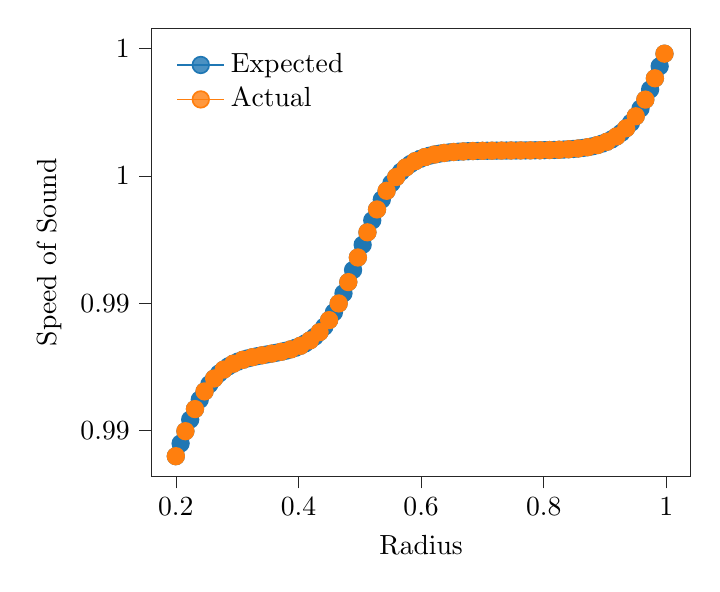
\begin{tikzpicture}

\definecolor{color0}{rgb}{0.12156862745098,0.466666666666667,0.705882352941177}
\definecolor{color1}{rgb}{1,0.498039215686275,0.0549019607843137}

\begin{axis}[
axis line style={white!15!black},
legend cell align={left},
legend style={
  fill opacity=0.8,
  draw opacity=1,
  text opacity=1,
  at={(0.03,0.97)},
  anchor=north west,
  draw=none
},
tick align=outside,
tick pos=left,
x grid style={white!80!black},
xlabel={Radius},
xmin=0.16, xmax=1.04,
xtick style={color=white!15!black},
y grid style={white!80!black},
ylabel={Speed of Sound},
ymin=0.98320056903035, ymax=1.00079997290332,
ytick style={color=white!15!black}
]
\addplot [semithick, color0, mark=*, mark size=3, mark repeat=5, mark options={solid}]
table {%
0.2 0.984000541933667
0.2015625 0.984100548886647
0.203125 0.984200432419622
0.2046875 0.984300068384446
0.20625 0.984399333875707
0.2078125 0.984498107834061
0.209375 0.984596271630271
0.2109375 0.984693709624082
0.2125 0.984790309692462
0.2140625 0.984885963722324
0.215625 0.984980568063398
0.2171875 0.985074023937652
0.21875 0.985166237802302
0.2203125 0.985257121664242
0.221875 0.985346593344428
0.2234375 0.985434576691501
0.225 0.985521001744648
0.2265625 0.985605804846342
0.228125 0.985688928706271
0.2296875 0.985770322418282
0.23125 0.985849941432696
0.2328125 0.985927747486754
0.234375 0.986003708496322
0.2359375 0.986077798412233
0.2375 0.986149997044859
0.2390625 0.986220289860638
0.240625 0.986288667754308
0.2421875 0.986355126800626
0.24375 0.986419667989276
0.2453125 0.986482296946548
0.246875 0.986543023647233
0.2484375 0.986601862119971
0.25 0.986658830149088
0.2515625 0.986713948975696
0.253125 0.98676724300061
0.2546875 0.98681873949133
0.25625 0.986868468295113
0.2578125 0.986916461559873
0.259375 0.986962753464396
0.2609375 0.987007379959106
0.2625 0.987050378518398
0.2640625 0.987091787905317
0.265625 0.987131647949157
0.2671875 0.987169999336396
0.26875 0.98720688341517
0.2703125 0.987242342013376
0.271875 0.987276417270339
0.2734375 0.987309151481869
0.275 0.987340586958444
0.2765625 0.987370765896143
0.278125 0.987399730259926
0.2796875 0.987427521678759
0.28125 0.987454181352077
0.2828125 0.987479749967015
0.284375 0.987504267625839
0.2859375 0.987527773782981
0.2875 0.987550307191088
0.2890625 0.987571905855486
0.290625 0.987592606996474
0.2921875 0.987612447018872
0.29375 0.987631461488276
0.2953125 0.987649685113462
0.296875 0.987667151734442
0.2984375 0.987683894315661
0.3 0.987699944943884
0.3015625 0.987715334830319
0.303125 0.987730094316565
0.3046875 0.987744252883996
0.30625 0.987757839166223
0.3078125 0.987770880964282
0.309375 0.987783405264264
0.3109375 0.987795438257075
0.3125 0.987807005360076
0.3140625 0.987818131240364
0.315625 0.987828839839472
0.3171875 0.987839154399291
0.31875 0.98784909748904
0.3203125 0.987858691033117
0.321875 0.9878679563397
0.3234375 0.987876914129958
0.325 0.987885584567766
0.3265625 0.987893987289837
0.328125 0.98790214143616
0.3296875 0.987910065680699
0.33125 0.987917778262275
0.3328125 0.987925297015572
0.334375 0.987932639402246
0.3359375 0.987939822542074
0.3375 0.987946863244137
0.3390625 0.987953778037998
0.340625 0.987960583204877
0.3421875 0.987967294808789
0.34375 0.98797392872766
0.3453125 0.987980500684408
0.346875 0.987987026277992
0.3484375 0.987993521014427
0.35 0.988000000337782
0.3515625 0.988006479661155
0.353125 0.988012974397646
0.3546875 0.988019499991323
0.35625 0.988026071948201
0.3578125 0.988032705867241
0.359375 0.988039417471358
0.3609375 0.988046222638482
0.3625 0.988053137432628
0.3640625 0.988060178135015
0.365625 0.988067361275209
0.3671875 0.98807470366229
0.36875 0.988082222416037
0.3703125 0.988089934998106
0.371875 0.988097859243185
0.3734375 0.988106013390094
0.375 0.988114416112798
0.3765625 0.988123086551289
0.378125 0.988132044342281
0.3796875 0.988141309649652
0.38125 0.988150903194572
0.3828125 0.98816084628522
0.384375 0.988171160845998
0.3859375 0.988181869446127
0.3875 0.9881929953275
0.3890625 0.988204562431654
0.390625 0.988216595425687
0.3921875 0.988229119726965
0.39375 0.988242161526395
0.3953125 0.988255747810073
0.396875 0.988269906379039
0.3984375 0.988284665866907
0.4 0.988300055755055
0.4015625 0.988316106385087
0.403125 0.988332848968214
0.4046875 0.988350315591207
0.40625 0.988368539218517
0.4078125 0.988387553690159
0.409375 0.988407393714916
0.4109375 0.988428094858389
0.4125 0.988449693525406
0.4140625 0.988472226936272
0.415625 0.988495733096318
0.4171875 0.988520250758199
0.41875 0.988545819376356
0.4203125 0.988572479053063
0.421875 0.988600270475462
0.4234375 0.988629234842998
0.425 0.988659413784646
0.4265625 0.988690849265375
0.428125 0.988723583481276
0.4296875 0.988757658742837
0.43125 0.98879311734588
0.4328125 0.988830001429742
0.434375 0.988868352822332
0.4359375 0.9889082128718
0.4375 0.988949622264638
0.4390625 0.988992620830155
0.440625 0.989037247331411
0.4421875 0.989083539242818
0.44375 0.989131532514817
0.4453125 0.989181261326212
0.446875 0.989232757824935
0.4484375 0.989286051858266
0.45 0.989341170693724
0.4515625 0.989398138732145
0.453125 0.989456977214666
0.4546875 0.989517703925637
0.45625 0.989580332893724
0.4578125 0.989644874093744
0.459375 0.989711333152017
0.4609375 0.989779711058255
0.4625 0.989850003887249
0.4640625 0.989922202533768
0.465625 0.989996292464284
0.4671875 0.990072253489208
0.46875 0.99015005955941
0.4703125 0.990229678590797
0.471875 0.990311072320652
0.4734375 0.99039419619934
0.475 0.990478999320756
0.4765625 0.990565424394636
0.478125 0.990653407763507
0.4796875 0.990742879466609
0.48125 0.99083376335264
0.4828125 0.990925977242617
0.484375 0.991019433143496
0.4859375 0.991114037512562
0.4875 0.991209691571851
0.4890625 0.991306291671168
0.490625 0.991403729697502
0.4921875 0.991501893527903
0.49375 0.991600667522201
0.4953125 0.99169993305125
0.496875 0.991799569055799
0.4984375 0.991899452630537
0.5 0.991999459627421
0.5015625 0.992099465272067
0.503125 0.99219934478671
0.5046875 0.992298974013166
0.50625 0.992398230029186
0.5078125 0.992496991751752
0.509375 0.992595140521059
0.5109375 0.992692560659307
0.5125 0.992789139998857
0.5140625 0.99288477037483
0.515625 0.992979348077864
0.5171875 0.99307277426338
0.51875 0.993164955314424
0.5203125 0.993255803155917
0.521875 0.993345235518834
0.5234375 0.993433176153603
0.525 0.993519554992716
0.5265625 0.993604308263212
0.528125 0.993687378550314
0.5296875 0.993768714814062
0.53125 0.993848272361297
0.5328125 0.993926012775751
0.534375 0.994001903809366
0.5359375 0.99407591923823
0.5375 0.994148038686721
0.5390625 0.99421824742356
0.540625 0.994286536133559
0.5421875 0.994352900668823
0.54375 0.994417341783093
0.5453125 0.994479864852854
0.546875 0.994540479588594
0.5484375 0.994599199739509
0.55 0.994656042794637
0.5515625 0.994711029683234
0.553125 0.994764184476907
0.5546875 0.994815534095789
0.55625 0.994865108020749
0.5578125 0.99491293801338
0.559375 0.99495905784526
0.5609375 0.995003503037712
0.5625 0.995046310613072
0.5640625 0.995087518858254
0.565625 0.995127167101171
0.5671875 0.995165295500434
0.56875 0.99520194484852
0.5703125 0.995237156388507
0.571875 0.995270971644298
0.5734375 0.995303432264168
0.575 0.995334579877347
0.5765625 0.995364455963282
0.578125 0.995393101733155
0.5796875 0.995420558023162
0.58125 0.995446865199025
0.5828125 0.995472063071189
0.584375 0.9954961908201
0.5859375 0.995519286930997
0.5875 0.995541389137587
0.5890625 0.995562534374025
0.590625 0.995582758734604
0.5921875 0.995602097440566
0.59375 0.995620584813474
0.5953125 0.995638254254612
0.596875 0.995655138229866
0.5984375 0.995671268259608
0.6 0.995686674913096
0.6015625 0.995701387806942
0.603125 0.995715435607232
0.6046875 0.995728846034892
0.60625 0.99574164587393
0.6078125 0.995753860982223
0.609375 0.995765516304507
0.6109375 0.995776635887292
0.6125 0.995787242895424
0.6140625 0.995797359630043
0.615625 0.995807007547711
0.6171875 0.995816207280501
0.61875 0.995824978656858
0.6203125 0.995833340723064
0.621875 0.995841311765143
0.6234375 0.995848909331092
0.625 0.995856150253272
0.6265625 0.995863050670899
0.628125 0.995869626052497
0.6296875 0.99587589121825
0.63125 0.995881860362164
0.6328125 0.995887547073985
0.634375 0.995892964360806
0.6359375 0.995898124668321
0.6375 0.995903039901678
0.6390625 0.995907721445908
0.640625 0.995912180185882
0.6421875 0.995916426525794
0.64375 0.995920470408134
0.6453125 0.995924321332153
0.646875 0.995927988371789
0.6484375 0.995931480193072
0.65 0.995934805070983
0.6515625 0.995937970905779
0.653125 0.99594098523878
0.6546875 0.995943855267619
0.65625 0.995946587860976
0.6578125 0.995949189572774
0.659375 0.995951666655872
0.6609375 0.995954025075258
0.6625 0.99595627052074
0.6640625 0.995958408419154
0.665625 0.995960443946116
0.6671875 0.995962382037296
0.66875 0.995964227399259
0.6703125 0.995965984519872
0.671875 0.995967657678284
0.6734375 0.995969250954509
0.675 0.995970768238611
0.6765625 0.995972213239507
0.678125 0.995973589493407
0.6796875 0.995974900371901
0.68125 0.995976149089699
0.6828125 0.995977338712054
0.684375 0.995978472161855
0.6859375 0.995979552226434
0.6875 0.995980581564065
0.6890625 0.995981562710198
0.690625 0.995982498083416
0.6921875 0.995983389991139
0.69375 0.995984240635083
0.6953125 0.995985052116483
0.696875 0.995985826441091
0.6984375 0.99598656552396
0.7 0.995987271194022
0.7015625 0.995987945198473
0.703125 0.995988589206969
0.7046875 0.995989204815643
0.70625 0.995989793550959
0.7078125 0.995990356873398
0.709375 0.995990896180996
0.7109375 0.99599141281273
0.7125 0.99599190805178
0.7140625 0.99599238312864
0.715625 0.995992839224128
0.7171875 0.995993277472259
0.71875 0.995993698963021
0.7203125 0.99599410474504
0.721875 0.99599449582815
0.7234375 0.995994873185871
0.725 0.995995237757798
0.7265625 0.995995590451909
0.728125 0.995995932146805
0.7296875 0.995996263693868
0.73125 0.995996585919359
0.7328125 0.995996899626465
0.734375 0.995997205597271
0.7359375 0.9959975045947
0.7375 0.995997797364393
0.7390625 0.995998084636562
0.740625 0.995998367127788
0.7421875 0.995998645542801
0.74375 0.995998920576223
0.7453125 0.995999192914293
0.746875 0.995999463236562
0.7484375 0.995999732217585
0.75 0.996000000528589
0.7515625 0.996000268839138
0.753125 0.996000537818796
0.7546875 0.996000808138787
0.75625 0.996001080473659
0.7578125 0.996001355502957
0.759375 0.996001633912908
0.7609375 0.996001916398121
0.7625 0.996002203663312
0.7640625 0.996002496425045
0.765625 0.996002795413511
0.7671875 0.996003101374329
0.76875 0.996003415070396
0.7703125 0.996003737283773
0.771875 0.996004068817611
0.7734375 0.996004410498143
0.775 0.996004763176713
0.7765625 0.996005127731883
0.778125 0.996005505071589
0.7796875 0.996005896135382
0.78125 0.996006301896732
0.7828125 0.996006723365422
0.784375 0.996007161590024
0.7859375 0.996007617660467
0.7875 0.996008092710702
0.7890625 0.996008587921481
0.790625 0.996009104523228
0.7921875 0.996009643799046
0.79375 0.996010207087836
0.7953125 0.996010795787547
0.796875 0.996011411358571
0.7984375 0.996012055327279
0.8 0.996012729289704
0.8015625 0.996013434915398
0.803125 0.996014173951444
0.8046875 0.996014948226658
0.80625 0.99601575965597
0.8078125 0.996016610245002
0.809375 0.99601750209485
0.8109375 0.996018437407087
0.8125 0.996019418488979
0.8140625 0.99602044775895
0.815625 0.996021527752279
0.8171875 0.996022661127064
0.81875 0.996023850670446
0.8203125 0.996025099305121
0.821875 0.99602641009613
0.8234375 0.996027786257968
0.825 0.996029231161992
0.8265625 0.996030748344171
0.828125 0.996032341513167
0.8296875 0.996034014558775
0.83125 0.996035771560727
0.8328125 0.996037616797878
0.834375 0.996039554757779
0.8359375 0.996041590146669
0.8375 0.996043727899874
0.8390625 0.996045973192643
0.840625 0.996048331451433
0.8421875 0.996050808365651
0.84375 0.99605340989986
0.8453125 0.996056142306476
0.846875 0.996059012138958
0.8484375 0.99606202626549
0.85 0.996065191883192
0.8515625 0.996068516532841
0.853125 0.996072008114122
0.8546875 0.996075674901416
0.85625 0.996079525560123
0.8578125 0.996083569163517
0.859375 0.996087815210152
0.8609375 0.996092273641784
0.8625 0.996096954861836
0.8640625 0.996101869754369
0.865625 0.996107029703561
0.8671875 0.996112446613664
0.86875 0.99611813292943
0.8703125 0.996124101656964
0.871875 0.996130366384967
0.8734375 0.996136941306354
0.875 0.996143841240155
0.8765625 0.996151081653687
0.878125 0.996158678684891
0.8796875 0.996166649164795
0.88125 0.996175010639986
0.8828125 0.996183781395013
0.884375 0.996192980474604
0.8859375 0.99620262770557
0.8875 0.996212743718267
0.8890625 0.996223349967452
0.890625 0.996234468752366
0.8921875 0.996246123235863
0.89375 0.996258337462352
0.8953125 0.996271136374368
0.896875 0.996284545827466
0.8984375 0.99629859260322
0.9 0.996313304419992
0.9015625 0.996328709941177
0.903125 0.996344838780554
0.9046875 0.996361721504406
0.90625 0.996379389629974
0.9078125 0.996397875619856
0.909375 0.996417212871876
0.9109375 0.996437435703965
0.9125 0.99645857933354
0.9140625 0.996480679850876
0.915625 0.996503774185906
0.9171875 0.996527900067896
0.91875 0.996553095977414
0.9203125 0.996579401090003
0.921875 0.996606855210946
0.9234375 0.996635498700543
0.925 0.996665372389287
0.9265625 0.996696517482366
0.928125 0.996728975452927
0.9296875 0.996762787923574
0.93125 0.996797996535619
0.9328125 0.996834642805644
0.934375 0.99687276796903
0.9359375 0.996912412810164
0.9375 0.996953617479149
0.9390625 0.996996421294959
0.940625 0.997040862535105
0.9421875 0.997086978212043
0.94375 0.997134803836707
0.9453125 0.997184373169752
0.946875 0.997235717961291
0.9484375 0.997288867680121
0.95 0.997343849233688
0.9515625 0.99740068668026
0.953125 0.997459400935069
0.9546875 0.997520009472411
0.95625 0.997582526025983
0.9578125 0.997646960289984
0.959375 0.997713317623768
0.9609375 0.997781598763074
0.9625 0.997851799541075
0.9640625 0.997923910622686
0.965625 0.99799791725571
0.9671875 0.998073799042532
0.96875 0.998151529736121
0.9703125 0.998231077064117
0.971875 0.998312402584702
0.9734375 0.998395461577857
0.975 0.998480202975387
0.9765625 0.998566569332831
0.978125 0.998654496846022
0.9796875 0.998743915414651
0.98125 0.998834748754659
0.9828125 0.998926914560766
0.984375 0.999020324719782
0.9859375 0.99911488557469
0.9875 0.99921049823879
0.9890625 0.999307058958444
0.990625 0.999404459522227
0.9921875 0.999502587713568
0.99375 0.999601327803226
0.9953125 0.999700561077321
0.996875 0.999800166395987
0.9984375 0.999900020777216
1 1
};
\addlegendentry{Expected}
\addplot [semithick, color1, mark=*, mark size=3, mark repeat=10, mark options={solid}]
table {%
0.2 0.984000542019354
0.2015625 0.984100538570465
0.203125 0.984200411755927
0.2046875 0.984300037478986
0.20625 0.984399292884513
0.2078125 0.984498056961819
0.209375 0.984596211128208
0.2109375 0.98469363978739
0.2125 0.984790230857325
0.2140625 0.984885876262573
0.215625 0.98498047238688
0.2171875 0.985073920482345
0.21875 0.985166127032258
0.2203125 0.985257004065404
0.221875 0.985346469420391
0.2234375 0.985434446959279
0.225 0.98552086673049
0.2265625 0.985605665081666
0.228125 0.985688784723747
0.2296875 0.985770174748117
0.23125 0.985849790599148
0.2328125 0.985927594004909
0.234375 0.986003552869154
0.2359375 0.986077641127965
0.2375 0.986149838574637
0.2390625 0.986220130656513
0.240625 0.986288508247539
0.2421875 0.986354967400289
0.24375 0.986419509081172
0.2453125 0.986482138892399
0.246875 0.986542866784147
0.2484375 0.98660170676016
0.25 0.986658676579815
0.2515625 0.986713797459438
0.253125 0.986767093775402
0.2546875 0.986818592771284
0.25625 0.986868324271075
0.2578125 0.98691632040021
0.259375 0.986962615315875
0.2609375 0.987007244947868
0.2625 0.987050246750991
0.2640625 0.987091659469774
0.265625 0.987131522916112
0.2671875 0.987169877760217
0.26875 0.987206765335094
0.2703125 0.987242227454642
0.271875 0.987276306245304
0.2734375 0.987309043991106
0.275 0.987340482991801
0.2765625 0.987370665433774
0.278125 0.987399633273278
0.2796875 0.987427428131517
0.28125 0.987454091201058
0.2828125 0.987479663163019
0.284375 0.987504184114449
0.2859375 0.987527693505313
0.2875 0.98755023008449
0.2890625 0.987571831854191
0.290625 0.9875925360322
0.2921875 0.987612379021383
0.29375 0.987631396385893
0.2953125 0.987649622833532
0.296875 0.987667092203763
0.2984375 0.987683837460875
0.3 0.987699890691827
0.3015625 0.987715283108339
0.303125 0.987730045052807
0.3046875 0.987744206007658
0.30625 0.987757794607782
0.3078125 0.987770838655695
0.309375 0.987783365139148
0.3109375 0.98779540025086
0.3125 0.987806969410141
0.3140625 0.987818097286156
0.315625 0.987828807822605
0.3171875 0.987839124263634
0.31875 0.98784906918079
0.3203125 0.987858664500862
0.321875 0.987867931534466
0.3234375 0.987876891005252
0.325 0.987885563079613
0.3265625 0.987893967396799
0.328125 0.987902123099364
0.3296875 0.987910048863849
0.33125 0.987917762931659
0.3328125 0.987925283140076
0.334375 0.987932626953352
0.3359375 0.987939811493866
0.3375 0.987946853573297
0.3390625 0.987953769723811
0.340625 0.98796057622922
0.3421875 0.987967289156136
0.34375 0.987973924385075
0.3453125 0.987980497641544
0.346875 0.987987024527085
0.3484375 0.987993520550299
0.35 0.988000001157834
0.3515625 0.988006481765371
0.353125 0.98801297778859
0.3546875 0.988019504674139
0.35625 0.988026077930618
0.3578125 0.988032713159569
0.359375 0.988039426086497
0.3609375 0.988046232591919
0.3625 0.988053148742442
0.3640625 0.98806019082188
0.365625 0.988067375362393
0.3671875 0.988074719175661
0.36875 0.988082239384058
0.3703125 0.988089953451836
0.371875 0.988097879216269
0.3734375 0.988106034918762
0.375 0.988114439235851
0.3765625 0.988123111310083
0.378125 0.988132070780705
0.3796875 0.988141337814104
0.38125 0.988150933133922
0.3828125 0.988160878050769
0.384375 0.988171194491426
0.3859375 0.988181905027431
0.3875 0.988193032902921
0.3890625 0.988204602061585
0.390625 0.988216637172577
0.3921875 0.988229163655196
0.39375 0.988242207702146
0.3953125 0.988255796301162
0.396875 0.988269957254748
0.3984375 0.988284719197773
0.4 0.988300111612648
0.4015625 0.988316164841748
0.403125 0.98833291009677
0.4046875 0.988350379464653
0.40625 0.988368605909658
0.4078125 0.988387623271224
0.409375 0.988407466257124
0.4109375 0.988428170431479
0.4125 0.988449772197124
0.4140625 0.988472308771811
0.415625 0.988495818157714
0.4171875 0.988520339103674
0.41875 0.988545911059617
0.4203125 0.988572574122552
0.421875 0.988600368973554
0.4234375 0.988629336805148
0.425 0.988659519238492
0.4265625 0.988690958229793
0.428125 0.988723695965391
0.4296875 0.988757774744993
0.43125 0.988793236852577
0.4328125 0.988830124414544
0.434375 0.988868479244747
0.4359375 0.988908342676152
0.4375 0.988949755378929
0.4390625 0.98899275716494
0.440625 0.989037386778686
0.4421875 0.989083681674941
0.44375 0.989131677783485
0.4453125 0.989181409261496
0.446875 0.989232908234404
0.4484375 0.989286204526211
0.45 0.989341325380513
0.4515625 0.989398295173717
0.453125 0.989457135122194
0.4546875 0.989517862985384
0.45625 0.989580492767111
0.4578125 0.989645034417647
0.459375 0.989711493539319
0.4609375 0.98977987109867
0.4625 0.989850163148432
0.4640625 0.989922360562726
0.465625 0.989996448789093
0.4671875 0.990072407621048
0.46875 0.990150210994911
0.4703125 0.990229826814696
0.471875 0.990311216808754
0.4734375 0.990394336421754
0.475 0.990479134745392
0.4765625 0.990565554490936
0.478125 0.990653532006369
0.4796875 0.990742997340459
0.48125 0.99083387435562
0.4828125 0.990926080890818
0.484375 0.991019528975192
0.4859375 0.991114125092381
0.4875 0.991209770494826
0.4890625 0.991306361566602
0.490625 0.991403790232585
0.4921875 0.991501944411025
0.49375 0.991600708505906
0.4953125 0.991699963934777
0.496875 0.991799589687169
0.4984375 0.991899462908144
0.5 0.991999459501105
0.5015625 0.992099454743644
0.503125 0.992199323909957
0.5046875 0.992298942893246
0.50625 0.992398188821544
0.5078125 0.992496940660486
0.509375 0.992595079796797
0.5109375 0.99269249059664
0.5125 0.992789060933354
0.5140625 0.992884682679702
0.515625 0.992979252160325
0.5171875 0.993072670560762
0.51875 0.993164844290118
0.5203125 0.993255685295191
0.521875 0.99334511132459
0.5234375 0.99343304614214
0.525 0.99351941968955
0.5265625 0.993604168199006
0.528125 0.993687234256956
0.5296875 0.993768566820951
0.53125 0.993848121191855
0.5328125 0.993925858944195
0.534375 0.99400174781777
0.5359375 0.994075761573883
0.5375 0.994147879819793
0.5390625 0.994218087805088
0.540625 0.994286376193745
0.5421875 0.99435274081564
0.54375 0.994417182401192
0.5453125 0.994479706302753
0.546875 0.994540322206146
0.5484375 0.99459904383561
0.55 0.994655888655176
0.5515625 0.994710877569247
0.553125 0.994764034624923
0.5546875 0.994815386718341
0.55625 0.994864963307029
0.5578125 0.994912796130018
0.559375 0.994958918937205
0.5609375 0.995003367229198
0.5625 0.995046178008647
0.5640625 0.995087389543851
0.565625 0.995127041145225
0.5671875 0.995165172955
0.56875 0.99520182575041
0.5703125 0.995237040760414
0.571875 0.995270859495909
0.5734375 0.995303323593251
0.575 0.995334474670805
0.5765625 0.995364354198178
0.578125 0.995393003377691
0.5796875 0.995420463037613
0.58125 0.995446773536632
0.5828125 0.995471974678994
0.584375 0.995496105639743
0.5859375 0.99551920489945
0.5875 0.99554131018785
0.5890625 0.995562458435763
0.590625 0.995582685734742
0.5921875 0.995602027303832
0.59375 0.995620517462904
0.5953125 0.995638189612002
0.596875 0.99565507621619
0.5984375 0.99567120879539
0.6 0.99568661791875
0.6015625 0.995701333203077
0.603125 0.995715383314918
0.6046875 0.995728795975899
0.60625 0.995741597970942
0.6078125 0.995753815159019
0.609375 0.995765472486118
0.6109375 0.995776594000141
0.6125 0.995787202867441
0.6140625 0.995797321390759
0.615625 0.995806971028341
0.6171875 0.995816172414004
0.61875 0.995824945377991
0.6203125 0.995833308968413
0.621875 0.995841281473156
0.6234375 0.995848880442084
0.625 0.995856122709439
0.6265625 0.995863024416314
0.628125 0.995869601033097
0.6296875 0.995875867381824
0.63125 0.995881837658331
0.6328125 0.995887525454166
0.634375 0.995892943778198
0.6359375 0.995898105077859
0.6375 0.995903021260004
0.6390625 0.995907703711326
0.640625 0.995912163318324
0.6421875 0.995916410486774
0.64375 0.995920455160706
0.6453125 0.995924306840866
0.646875 0.995927974602643
0.6484375 0.995931467113475
0.65 0.995934792649703
0.6515625 0.9959379591129
0.653125 0.995940974045658
0.6546875 0.995943844646839
0.65625 0.995946577786306
0.6578125 0.995949180019123
0.659375 0.99595165759925
0.6609375 0.995954016492733
0.6625 0.995956262390396
0.6640625 0.995958400720057
0.665625 0.995960436658271
0.6671875 0.99596237514161
0.66875 0.995964220877508
0.6703125 0.995965978354663
0.671875 0.995967651853024
0.6734375 0.99596924545337
0.675 0.995970763046498
0.6765625 0.99597220834203
0.678125 0.995973584876848
0.6796875 0.995974896023187
0.68125 0.995976144996378
0.6828125 0.995977334862262
0.684375 0.995978468544298
0.6859375 0.995979548830358
0.6875 0.995980578379236
0.6890625 0.995981559726879
0.690625 0.995982495292344
0.6921875 0.995983387383507
0.69375 0.995984238202519
0.6953125 0.995985049851032
0.696875 0.995985824335194
0.6984375 0.995986563570442
0.7 0.995987269386074
0.7015625 0.995987943529633
0.703125 0.995988587671111
0.7046875 0.995989203406963
0.70625 0.99598979226396
0.7078125 0.995990355702877
0.709375 0.995990895122031
0.7109375 0.995991411860674
0.7125 0.995991907202242
0.7140625 0.995992382377482
0.715625 0.99599283856745
0.7171875 0.995993276906392
0.71875 0.99599369848452
0.7203125 0.995994104350672
0.721875 0.99599449551489
0.7234375 0.995994872950893
0.725 0.995995237598466
0.7265625 0.995995590365778
0.728125 0.995995932131606
0.7296875 0.995996263747507
0.73125 0.995996586039915
0.7328125 0.995996899812179
0.734375 0.995997205846547
0.7359375 0.995997504906098
0.7375 0.995997797736628
0.7390625 0.995998085068498
0.740625 0.995998367618437
0.7421875 0.995998646091321
0.74375 0.995998921181916
0.7453125 0.995999193576601
0.746875 0.99599946395507
0.7484375 0.995999732992015
0.75 0.996000001358802
0.7515625 0.996000269725134
0.753125 0.996000538760714
0.7546875 0.996000809136904
0.75625 0.996001081528391
0.7578125 0.99600135661486
0.759375 0.99600163508268
0.7609375 0.996001917626605
0.7625 0.996002204951495
0.7640625 0.996002497774063
0.765625 0.996002796824648
0.7671875 0.996003102849025
0.76875 0.996003416610248
0.7703125 0.996003738890537
0.771875 0.996004070493211
0.7734375 0.99600441224467
0.775 0.996004764996435
0.7765625 0.996005129627247
0.778125 0.996005507045229
0.7796875 0.996005898190124
0.78125 0.996006304035602
0.7828125 0.996006725591651
0.784375 0.996007163907057
0.7859375 0.996007620071971
0.7875 0.996008095220578
0.7890625 0.996008590533865
0.790625 0.99600910724251
0.7921875 0.996009646629875
0.79375 0.99601021003513
0.7953125 0.996010798856509
0.796875 0.996011414554698
0.7984375 0.996012058656374
0.8 0.996012732757891
0.8015625 0.996013438529137
0.803125 0.996014177717544
0.8046875 0.996014952152294
0.80625 0.996015763748697
0.8078125 0.996016614512774
0.809375 0.996017506546037
0.8109375 0.996018442050494
0.8125 0.996019423333868
0.8140625 0.996020452815054
0.815625 0.996021533029831
0.8171875 0.996022666636814
0.81875 0.996023856423687
0.8203125 0.996025105313711
0.821875 0.996026416372521
0.8234375 0.996027792815226
0.825 0.996029238013831
0.8265625 0.996030755504977
0.828125 0.99603234899803
0.8296875 0.996034022383518
0.83125 0.996035779741937
0.8328125 0.996037625352941
0.834375 0.996039563704913
0.8359375 0.996041599504958
0.8375 0.996043737689303
0.8390625 0.99604598343414
0.840625 0.996048342166902
0.8421875 0.996050819578012
0.84375 0.996053421633092
0.8453125 0.996056154585657
0.846875 0.996059024990304
0.8484375 0.996062039716402
0.85 0.996065205962296
0.8515625 0.996068531270032
0.853125 0.996072023540612
0.8546875 0.996075691049775
0.85625 0.996079542464325
0.8578125 0.996083586858985
0.859375 0.996087833733802
0.8609375 0.996092293032069
0.8625 0.996096975158789
0.8640625 0.996101890999645
0.865625 0.996107051940475
0.8671875 0.996112469887234
0.86875 0.996118157286407
0.8703125 0.996124127145869
0.871875 0.99613039305612
0.8734375 0.996136969211897
0.875 0.996143870434077
0.8765625 0.996151112191834
0.878125 0.996158710624979
0.8796875 0.996166682566409
0.88125 0.996175045564575
0.8828125 0.996183817905873
0.884375 0.996193018636852
0.8859375 0.996202667586109
0.8875 0.996212785385732
0.8890625 0.996223393492147
0.890625 0.996234514206185
0.8921875 0.996246170692186
0.89375 0.996258386995937
0.8953125 0.996271188061206
0.896875 0.996284599744623
0.8984375 0.996298648828654
0.9 0.996313363032339
0.9015625 0.996328771019508
0.903125 0.99634490240411
0.9046875 0.996361787752286
0.90625 0.996379458580801
0.9078125 0.996397947351397
0.909375 0.996417287460625
0.9109375 0.996437513224683
0.9125 0.996458659858756
0.9140625 0.996480763450336
0.915625 0.996503860925981
0.9171875 0.996527990010936
0.91875 0.996553189181057
0.9203125 0.996579497606432
0.921875 0.996606955086097
0.9234375 0.996635601973261
0.925 0.996665479090439
0.9265625 0.9966966276339
0.928125 0.996729089066892
0.9296875 0.9967629050011
0.93125 0.996798117065855
0.9328125 0.996834766764676
0.934375 0.996872895318767
0.9359375 0.996912543497216
0.9375 0.996953751433694
0.9390625 0.996996558429622
0.940625 0.997041002743852
0.9421875 0.997087121369108
0.94375 0.997134949795571
0.9453125 0.997184521762187
0.946875 0.997235868996483
0.9484375 0.997289020943902
0.95 0.997344004487888
0.9515625 0.997400843662211
0.953125 0.997459559357272
0.9546875 0.997520169022392
0.95625 0.997582686366363
0.9578125 0.997647121058781
0.959375 0.997713478434953
0.9609375 0.997781759207394
0.9625 0.997851959187171
0.9640625 0.997924069018498
0.965625 0.997998073930204
0.9671875 0.998073953507733
0.96875 0.998151681489463
0.9703125 0.998231225591102
0.971875 0.99831254736186
0.9734375 0.998395602075987
0.975 0.998480338663054
0.9765625 0.998566699680098
0.978125 0.998654621328378
0.9796875 0.998744033517082
0.98125 0.998834859975838
0.9828125 0.998927018417289
0.984375 0.999020420750399
0.9859375 0.999114973344484
0.9875 0.999210577343224
0.9890625 0.999307129027227
0.990625 0.999404520222934
0.9921875 0.999502638754955
0.99375 0.999601368938184
0.9953125 0.999700592105417
0.996875 0.999800187165552
0.9984375 0.999900031186939
1 1
};
\addlegendentry{Actual}
\end{axis}

\end{tikzpicture}

    \end{center}
\end{figure}

\begin{figure}
    \begin{center}
        % This file was created with tikzplotlib v0.9.12.
\begin{tikzpicture}

\definecolor{color0}{rgb}{0.12156862745098,0.466666666666667,0.705882352941177}

\begin{groupplot}[group style={group size=1 by 2}]
\nextgroupplot[
axis line style={white!15!black},
legend cell align={left},
legend style={fill opacity=0.8, draw opacity=1, text opacity=1, draw=none},
log basis y={10},
scaled x ticks=manual:{}{\pgfmathparse{#1}},
tick align=outside,
tick pos=left,
title={Rate Of Convergence},
x grid style={white!80!black},
xmin=0.49602339181245, xmax=0.60495126705655,
xtick style={color=white!15!black},
xticklabels={},
y grid style={white!80!black},
ymin=1.93465772282466, ymax=2.50490389113768,
ymode=log,
ytick style={color=white!15!black}
]
\addplot [semithick, color0]
table {%
0.6 2.220755792495
0.555555555556 2.163324274032
0.529411764706 2.475663773488
0.515151515152 1.957508006467
0.507692307692 1.997639457419
0.503875968992 1.996551880759
0.501945525292 1.997726606828
0.500974658869 1.998727064418
};
\addlegendentry{Speed Of Sound}

\nextgroupplot[
axis line style={white!15!black},
legend cell align={left},
legend style={fill opacity=0.8, draw opacity=1, text opacity=1, draw=none},
log basis y={10},
tick align=outside,
tick pos=left,
x grid style={white!80!black},
xlabel={Del r},
xmin=0.49602339181245, xmax=0.60495126705655,
xtick style={color=white!15!black},
y grid style={white!80!black},
ymin=0.362953235346687, ymax=0.506191289267272,
ymode=log,
ytick style={color=white!15!black}
]
\addplot [semithick, color0]
table {%
0.6 0.368482797082
0.555555555556 0.423998453276
0.529411764706 0.458768919907
0.515151515152 0.478465639055
0.507692307692 0.488986846835
0.503875968992 0.494429721197
0.501945525292 0.497198646885
0.500974658869 0.498595233207
};
\addlegendentry{LEE}
\end{groupplot}

\end{tikzpicture}

    \end{center}
\end{figure}

\begin{figure}
    \begin{center}
        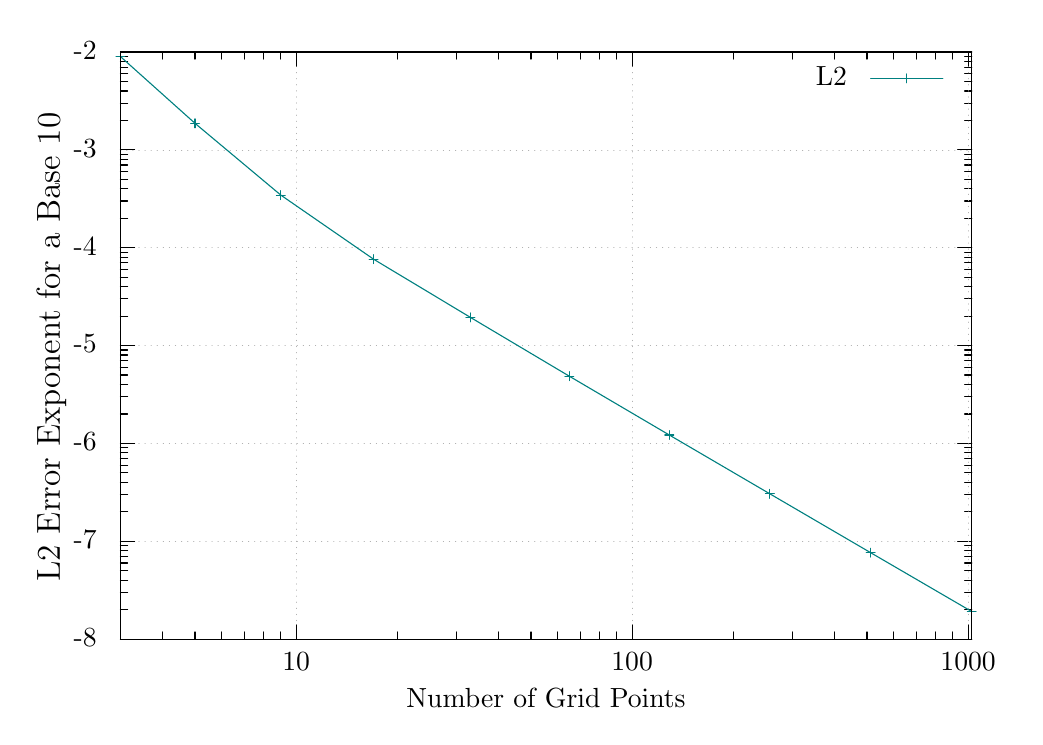
\begin{tikzpicture}[gnuplot]
%% generated with GNUPLOT 5.2p8 (Lua 5.3; terminal rev. Nov 2018, script rev. 108)
%% Tue 21 Sep 2021 05:01:33 PM EDT
\path (0.000,0.000) rectangle (12.500,8.750);
\gpcolor{color=gp lt color axes}
\gpsetlinetype{gp lt axes}
\gpsetdashtype{gp dt axes}
\gpsetlinewidth{0.50}
\draw[gp path] (1.136,0.985)--(11.947,0.985);
\gpcolor{color=gp lt color border}
\gpsetlinetype{gp lt border}
\gpsetdashtype{gp dt solid}
\gpsetlinewidth{1.00}
\draw[gp path] (1.136,0.985)--(1.316,0.985);
\draw[gp path] (11.947,0.985)--(11.767,0.985);
\node[gp node right] at (0.952,0.985) {{-8}};
\draw[gp path] (1.136,1.359)--(1.226,1.359);
\draw[gp path] (11.947,1.359)--(11.857,1.359);
\draw[gp path] (1.136,1.578)--(1.226,1.578);
\draw[gp path] (11.947,1.578)--(11.857,1.578);
\draw[gp path] (1.136,1.733)--(1.226,1.733);
\draw[gp path] (11.947,1.733)--(11.857,1.733);
\draw[gp path] (1.136,1.854)--(1.226,1.854);
\draw[gp path] (11.947,1.854)--(11.857,1.854);
\draw[gp path] (1.136,1.952)--(1.226,1.952);
\draw[gp path] (11.947,1.952)--(11.857,1.952);
\draw[gp path] (1.136,2.035)--(1.226,2.035);
\draw[gp path] (11.947,2.035)--(11.857,2.035);
\draw[gp path] (1.136,2.107)--(1.226,2.107);
\draw[gp path] (11.947,2.107)--(11.857,2.107);
\draw[gp path] (1.136,2.171)--(1.226,2.171);
\draw[gp path] (11.947,2.171)--(11.857,2.171);
\gpcolor{color=gp lt color axes}
\gpsetlinetype{gp lt axes}
\gpsetdashtype{gp dt axes}
\gpsetlinewidth{0.50}
\draw[gp path] (1.136,2.228)--(11.947,2.228);
\gpcolor{color=gp lt color border}
\gpsetlinetype{gp lt border}
\gpsetdashtype{gp dt solid}
\gpsetlinewidth{1.00}
\draw[gp path] (1.136,2.228)--(1.316,2.228);
\draw[gp path] (11.947,2.228)--(11.767,2.228);
\node[gp node right] at (0.952,2.228) {{-7}};
\draw[gp path] (1.136,2.602)--(1.226,2.602);
\draw[gp path] (11.947,2.602)--(11.857,2.602);
\draw[gp path] (1.136,2.821)--(1.226,2.821);
\draw[gp path] (11.947,2.821)--(11.857,2.821);
\draw[gp path] (1.136,2.976)--(1.226,2.976);
\draw[gp path] (11.947,2.976)--(11.857,2.976);
\draw[gp path] (1.136,3.096)--(1.226,3.096);
\draw[gp path] (11.947,3.096)--(11.857,3.096);
\draw[gp path] (1.136,3.195)--(1.226,3.195);
\draw[gp path] (11.947,3.195)--(11.857,3.195);
\draw[gp path] (1.136,3.278)--(1.226,3.278);
\draw[gp path] (11.947,3.278)--(11.857,3.278);
\draw[gp path] (1.136,3.350)--(1.226,3.350);
\draw[gp path] (11.947,3.350)--(11.857,3.350);
\draw[gp path] (1.136,3.413)--(1.226,3.413);
\draw[gp path] (11.947,3.413)--(11.857,3.413);
\gpcolor{color=gp lt color axes}
\gpsetlinetype{gp lt axes}
\gpsetdashtype{gp dt axes}
\gpsetlinewidth{0.50}
\draw[gp path] (1.136,3.470)--(11.947,3.470);
\gpcolor{color=gp lt color border}
\gpsetlinetype{gp lt border}
\gpsetdashtype{gp dt solid}
\gpsetlinewidth{1.00}
\draw[gp path] (1.136,3.470)--(1.316,3.470);
\draw[gp path] (11.947,3.470)--(11.767,3.470);
\node[gp node right] at (0.952,3.470) {{-6}};
\draw[gp path] (1.136,3.844)--(1.226,3.844);
\draw[gp path] (11.947,3.844)--(11.857,3.844);
\draw[gp path] (1.136,4.063)--(1.226,4.063);
\draw[gp path] (11.947,4.063)--(11.857,4.063);
\draw[gp path] (1.136,4.218)--(1.226,4.218);
\draw[gp path] (11.947,4.218)--(11.857,4.218);
\draw[gp path] (1.136,4.339)--(1.226,4.339);
\draw[gp path] (11.947,4.339)--(11.857,4.339);
\draw[gp path] (1.136,4.437)--(1.226,4.437);
\draw[gp path] (11.947,4.437)--(11.857,4.437);
\draw[gp path] (1.136,4.521)--(1.226,4.521);
\draw[gp path] (11.947,4.521)--(11.857,4.521);
\draw[gp path] (1.136,4.593)--(1.226,4.593);
\draw[gp path] (11.947,4.593)--(11.857,4.593);
\draw[gp path] (1.136,4.656)--(1.226,4.656);
\draw[gp path] (11.947,4.656)--(11.857,4.656);
\gpcolor{color=gp lt color axes}
\gpsetlinetype{gp lt axes}
\gpsetdashtype{gp dt axes}
\gpsetlinewidth{0.50}
\draw[gp path] (1.136,4.713)--(11.947,4.713);
\gpcolor{color=gp lt color border}
\gpsetlinetype{gp lt border}
\gpsetdashtype{gp dt solid}
\gpsetlinewidth{1.00}
\draw[gp path] (1.136,4.713)--(1.316,4.713);
\draw[gp path] (11.947,4.713)--(11.767,4.713);
\node[gp node right] at (0.952,4.713) {{-5}};
\draw[gp path] (1.136,5.087)--(1.226,5.087);
\draw[gp path] (11.947,5.087)--(11.857,5.087);
\draw[gp path] (1.136,5.306)--(1.226,5.306);
\draw[gp path] (11.947,5.306)--(11.857,5.306);
\draw[gp path] (1.136,5.461)--(1.226,5.461);
\draw[gp path] (11.947,5.461)--(11.857,5.461);
\draw[gp path] (1.136,5.582)--(1.226,5.582);
\draw[gp path] (11.947,5.582)--(11.857,5.582);
\draw[gp path] (1.136,5.680)--(1.226,5.680);
\draw[gp path] (11.947,5.680)--(11.857,5.680);
\draw[gp path] (1.136,5.763)--(1.226,5.763);
\draw[gp path] (11.947,5.763)--(11.857,5.763);
\draw[gp path] (1.136,5.835)--(1.226,5.835);
\draw[gp path] (11.947,5.835)--(11.857,5.835);
\draw[gp path] (1.136,5.899)--(1.226,5.899);
\draw[gp path] (11.947,5.899)--(11.857,5.899);
\gpcolor{color=gp lt color axes}
\gpsetlinetype{gp lt axes}
\gpsetdashtype{gp dt axes}
\gpsetlinewidth{0.50}
\draw[gp path] (1.136,5.956)--(11.947,5.956);
\gpcolor{color=gp lt color border}
\gpsetlinetype{gp lt border}
\gpsetdashtype{gp dt solid}
\gpsetlinewidth{1.00}
\draw[gp path] (1.136,5.956)--(1.316,5.956);
\draw[gp path] (11.947,5.956)--(11.767,5.956);
\node[gp node right] at (0.952,5.956) {{-4}};
\draw[gp path] (1.136,6.330)--(1.226,6.330);
\draw[gp path] (11.947,6.330)--(11.857,6.330);
\draw[gp path] (1.136,6.549)--(1.226,6.549);
\draw[gp path] (11.947,6.549)--(11.857,6.549);
\draw[gp path] (1.136,6.704)--(1.226,6.704);
\draw[gp path] (11.947,6.704)--(11.857,6.704);
\draw[gp path] (1.136,6.824)--(1.226,6.824);
\draw[gp path] (11.947,6.824)--(11.857,6.824);
\draw[gp path] (1.136,6.923)--(1.226,6.923);
\draw[gp path] (11.947,6.923)--(11.857,6.923);
\draw[gp path] (1.136,7.006)--(1.226,7.006);
\draw[gp path] (11.947,7.006)--(11.857,7.006);
\draw[gp path] (1.136,7.078)--(1.226,7.078);
\draw[gp path] (11.947,7.078)--(11.857,7.078);
\draw[gp path] (1.136,7.141)--(1.226,7.141);
\draw[gp path] (11.947,7.141)--(11.857,7.141);
\gpcolor{color=gp lt color axes}
\gpsetlinetype{gp lt axes}
\gpsetdashtype{gp dt axes}
\gpsetlinewidth{0.50}
\draw[gp path] (1.136,7.198)--(11.947,7.198);
\gpcolor{color=gp lt color border}
\gpsetlinetype{gp lt border}
\gpsetdashtype{gp dt solid}
\gpsetlinewidth{1.00}
\draw[gp path] (1.136,7.198)--(1.316,7.198);
\draw[gp path] (11.947,7.198)--(11.767,7.198);
\node[gp node right] at (0.952,7.198) {{-3}};
\draw[gp path] (1.136,7.572)--(1.226,7.572);
\draw[gp path] (11.947,7.572)--(11.857,7.572);
\draw[gp path] (1.136,7.791)--(1.226,7.791);
\draw[gp path] (11.947,7.791)--(11.857,7.791);
\draw[gp path] (1.136,7.946)--(1.226,7.946);
\draw[gp path] (11.947,7.946)--(11.857,7.946);
\draw[gp path] (1.136,8.067)--(1.226,8.067);
\draw[gp path] (11.947,8.067)--(11.857,8.067);
\draw[gp path] (1.136,8.165)--(1.226,8.165);
\draw[gp path] (11.947,8.165)--(11.857,8.165);
\draw[gp path] (1.136,8.249)--(1.226,8.249);
\draw[gp path] (11.947,8.249)--(11.857,8.249);
\draw[gp path] (1.136,8.321)--(1.226,8.321);
\draw[gp path] (11.947,8.321)--(11.857,8.321);
\draw[gp path] (1.136,8.384)--(1.226,8.384);
\draw[gp path] (11.947,8.384)--(11.857,8.384);
\gpcolor{color=gp lt color axes}
\gpsetlinetype{gp lt axes}
\gpsetdashtype{gp dt axes}
\gpsetlinewidth{0.50}
\draw[gp path] (1.136,8.441)--(11.947,8.441);
\gpcolor{color=gp lt color border}
\gpsetlinetype{gp lt border}
\gpsetdashtype{gp dt solid}
\gpsetlinewidth{1.00}
\draw[gp path] (1.136,8.441)--(1.316,8.441);
\draw[gp path] (11.947,8.441)--(11.767,8.441);
\node[gp node right] at (0.952,8.441) {{-2}};
\draw[gp path] (1.136,0.985)--(1.136,1.075);
\draw[gp path] (1.136,8.441)--(1.136,8.351);
\draw[gp path] (1.669,0.985)--(1.669,1.075);
\draw[gp path] (1.669,8.441)--(1.669,8.351);
\draw[gp path] (2.083,0.985)--(2.083,1.075);
\draw[gp path] (2.083,8.441)--(2.083,8.351);
\draw[gp path] (2.421,0.985)--(2.421,1.075);
\draw[gp path] (2.421,8.441)--(2.421,8.351);
\draw[gp path] (2.706,0.985)--(2.706,1.075);
\draw[gp path] (2.706,8.441)--(2.706,8.351);
\draw[gp path] (2.954,0.985)--(2.954,1.075);
\draw[gp path] (2.954,8.441)--(2.954,8.351);
\draw[gp path] (3.172,0.985)--(3.172,1.075);
\draw[gp path] (3.172,8.441)--(3.172,8.351);
\gpcolor{color=gp lt color axes}
\gpsetlinetype{gp lt axes}
\gpsetdashtype{gp dt axes}
\gpsetlinewidth{0.50}
\draw[gp path] (3.367,0.985)--(3.367,8.441);
\gpcolor{color=gp lt color border}
\gpsetlinetype{gp lt border}
\gpsetdashtype{gp dt solid}
\gpsetlinewidth{1.00}
\draw[gp path] (3.367,0.985)--(3.367,1.165);
\draw[gp path] (3.367,8.441)--(3.367,8.261);
\node[gp node center] at (3.367,0.677) {$10$};
\draw[gp path] (4.652,0.985)--(4.652,1.075);
\draw[gp path] (4.652,8.441)--(4.652,8.351);
\draw[gp path] (5.403,0.985)--(5.403,1.075);
\draw[gp path] (5.403,8.441)--(5.403,8.351);
\draw[gp path] (5.936,0.985)--(5.936,1.075);
\draw[gp path] (5.936,8.441)--(5.936,8.351);
\draw[gp path] (6.350,0.985)--(6.350,1.075);
\draw[gp path] (6.350,8.441)--(6.350,8.351);
\draw[gp path] (6.688,0.985)--(6.688,1.075);
\draw[gp path] (6.688,8.441)--(6.688,8.351);
\draw[gp path] (6.973,0.985)--(6.973,1.075);
\draw[gp path] (6.973,8.441)--(6.973,8.351);
\draw[gp path] (7.221,0.985)--(7.221,1.075);
\draw[gp path] (7.221,8.441)--(7.221,8.351);
\draw[gp path] (7.439,0.985)--(7.439,1.075);
\draw[gp path] (7.439,8.441)--(7.439,8.351);
\gpcolor{color=gp lt color axes}
\gpsetlinetype{gp lt axes}
\gpsetdashtype{gp dt axes}
\gpsetlinewidth{0.50}
\draw[gp path] (7.634,0.985)--(7.634,8.441);
\gpcolor{color=gp lt color border}
\gpsetlinetype{gp lt border}
\gpsetdashtype{gp dt solid}
\gpsetlinewidth{1.00}
\draw[gp path] (7.634,0.985)--(7.634,1.165);
\draw[gp path] (7.634,8.441)--(7.634,8.261);
\node[gp node center] at (7.634,0.677) {$100$};
\draw[gp path] (8.919,0.985)--(8.919,1.075);
\draw[gp path] (8.919,8.441)--(8.919,8.351);
\draw[gp path] (9.670,0.985)--(9.670,1.075);
\draw[gp path] (9.670,8.441)--(9.670,8.351);
\draw[gp path] (10.203,0.985)--(10.203,1.075);
\draw[gp path] (10.203,8.441)--(10.203,8.351);
\draw[gp path] (10.617,0.985)--(10.617,1.075);
\draw[gp path] (10.617,8.441)--(10.617,8.351);
\draw[gp path] (10.955,0.985)--(10.955,1.075);
\draw[gp path] (10.955,8.441)--(10.955,8.351);
\draw[gp path] (11.240,0.985)--(11.240,1.075);
\draw[gp path] (11.240,8.441)--(11.240,8.351);
\draw[gp path] (11.488,0.985)--(11.488,1.075);
\draw[gp path] (11.488,8.441)--(11.488,8.351);
\draw[gp path] (11.706,0.985)--(11.706,1.075);
\draw[gp path] (11.706,8.441)--(11.706,8.351);
\gpcolor{color=gp lt color axes}
\gpsetlinetype{gp lt axes}
\gpsetdashtype{gp dt axes}
\gpsetlinewidth{0.50}
\draw[gp path] (11.901,0.985)--(11.901,8.441);
\gpcolor{color=gp lt color border}
\gpsetlinetype{gp lt border}
\gpsetdashtype{gp dt solid}
\gpsetlinewidth{1.00}
\draw[gp path] (11.901,0.985)--(11.901,1.165);
\draw[gp path] (11.901,8.441)--(11.901,8.261);
\node[gp node center] at (11.901,0.677) {$1000$};
\draw[gp path] (1.136,8.441)--(1.136,0.985)--(11.947,0.985)--(11.947,8.441)--cycle;
\node[gp node center,rotate=-270,font={\fontsize{12.0pt}{14.4pt}\selectfont}] at (0.292,4.713) {L2 Error Exponent for a Base 10};
\node[gp node center] at (6.541,0.215) {Number of Grid Points};
\node[gp node right] at (10.479,8.107) {L2};
\gpcolor{rgb color={0.000,0.502,0.502}}
\draw[gp path] (10.663,8.107)--(11.579,8.107);
\draw[gp path] (1.136,8.383)--(2.083,7.535)--(3.172,6.624)--(4.350,5.810)--(5.580,5.071)%
  --(6.836,4.324)--(8.106,3.577)--(9.383,2.830)--(10.664,2.082)--(11.947,1.335);
\gpsetpointsize{4.00}
\gppoint{gp mark 1}{(1.136,8.383)}
\gppoint{gp mark 1}{(2.083,7.535)}
\gppoint{gp mark 1}{(3.172,6.624)}
\gppoint{gp mark 1}{(4.350,5.810)}
\gppoint{gp mark 1}{(5.580,5.071)}
\gppoint{gp mark 1}{(6.836,4.324)}
\gppoint{gp mark 1}{(8.106,3.577)}
\gppoint{gp mark 1}{(9.383,2.830)}
\gppoint{gp mark 1}{(10.664,2.082)}
\gppoint{gp mark 1}{(11.947,1.335)}
\gppoint{gp mark 1}{(11.121,8.107)}
\gpcolor{color=gp lt color border}
\draw[gp path] (1.136,8.441)--(1.136,0.985)--(11.947,0.985)--(11.947,8.441)--cycle;
%% coordinates of the plot area
\gpdefrectangularnode{gp plot 1}{\pgfpoint{1.136cm}{0.985cm}}{\pgfpoint{11.947cm}{8.441cm}}
\end{tikzpicture}
%% gnuplot variables

    \end{center}
\end{figure}




\begin{figure}
    \begin{center}
       % This file was created with tikzplotlib v0.9.12.
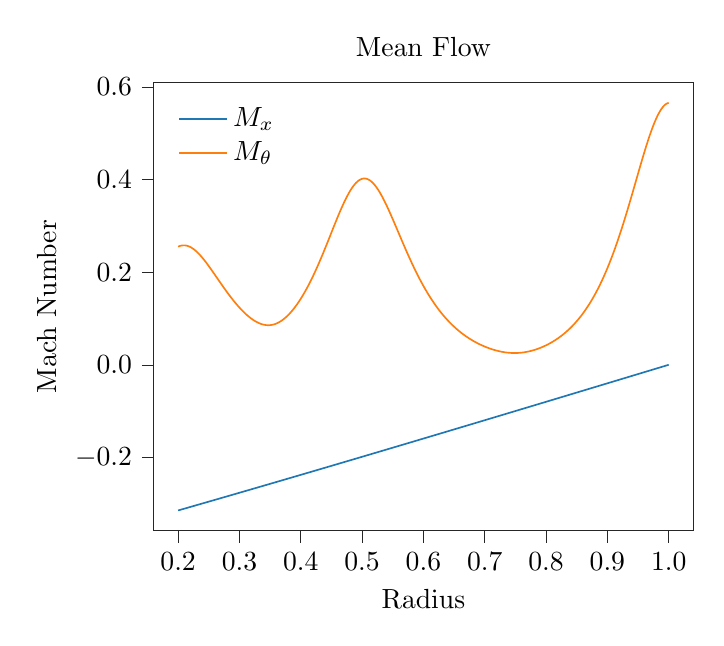
\begin{tikzpicture}

\definecolor{color0}{rgb}{0.12156862745098,0.466666666666667,0.705882352941177}
\definecolor{color1}{rgb}{1,0.498039215686275,0.0549019607843137}

\begin{axis}[
axis line style={white!15!black},
legend cell align={left},
legend style={
  fill opacity=0.8,
  draw opacity=1,
  text opacity=1,
  at={(0.03,0.97)},
  anchor=north west,
  draw=none
},
tick align=outside,
tick pos=left,
title={Mean Flow },
x grid style={white!80!black},
xlabel={Radius},
xmin=0.16, xmax=1.04,
xtick style={color=white!15!black},
xtick={0.1,0.2,0.3,0.4,0.5,0.6,0.7,0.8,0.9,1,1.1},
xticklabels={0.1,0.2,0.3,0.4,0.5,0.6,0.7,0.8,0.9,1.0,1.1},
y grid style={white!80!black},
ylabel={Mach Number},
ymin=-0.358579171685103, ymax=0.609698172253824,
ytick style={color=white!15!black},
ytick={-0.4,-0.2,0,0.2,0.4,0.6,0.8},
yticklabels={\ensuremath{-}0.4,\ensuremath{-}0.2,0.0,0.2,0.4,0.6,0.8}
]
\addplot [semithick, color0]
table {%
0.2 -0.314566565142425
0.2015625 -0.313973231598063
0.203125 -0.313379775407908
0.2046875 -0.312786196803778
0.20625 -0.31219249601754
0.2078125 -0.311598673281109
0.209375 -0.311004728826447
0.2109375 -0.310410662885563
0.2125 -0.309816475690513
0.2140625 -0.309222167473404
0.215625 -0.308627738466385
0.2171875 -0.308033188901657
0.21875 -0.307438519011464
0.2203125 -0.306843729028101
0.221875 -0.306248819183906
0.2234375 -0.305653789711266
0.225 -0.305058640842615
0.2265625 -0.304463372810433
0.228125 -0.303867985847246
0.2296875 -0.303272480185627
0.23125 -0.302676856058197
0.2328125 -0.302081113697619
0.234375 -0.301485253336607
0.2359375 -0.300889275207918
0.2375 -0.300293179544357
0.2390625 -0.299696966578772
0.240625 -0.29910063654406
0.2421875 -0.298504189673163
0.24375 -0.297907626199066
0.2453125 -0.297310946354804
0.246875 -0.296714150373453
0.2484375 -0.296117238488138
0.25 -0.295520210932026
0.2515625 -0.294923067938333
0.253125 -0.294325809740317
0.2546875 -0.293728436571281
0.25625 -0.293130948664575
0.2578125 -0.292533346253593
0.259375 -0.291935629571772
0.2609375 -0.291337798852597
0.2625 -0.290739854329594
0.2640625 -0.290141796236336
0.265625 -0.289543624806439
0.2671875 -0.288945340273564
0.26875 -0.288346942871416
0.2703125 -0.287748432833744
0.271875 -0.28714981039434
0.2734375 -0.286551075787042
0.275 -0.28595222924573
0.2765625 -0.285353271004329
0.278125 -0.284754201296807
0.2796875 -0.284155020357175
0.28125 -0.283555728419489
0.2828125 -0.282956325717846
0.284375 -0.282356812486389
0.2859375 -0.281757188959303
0.2875 -0.281157455370815
0.2890625 -0.280557611955196
0.290625 -0.27995765894676
0.2921875 -0.279357596579864
0.29375 -0.278757425088908
0.2953125 -0.278157144708332
0.296875 -0.277556755672622
0.2984375 -0.276956258216305
0.3 -0.27635565257395
0.3015625 -0.275754938980168
0.303125 -0.275154117669613
0.3046875 -0.274553188876981
0.30625 -0.273952152837011
0.3078125 -0.273351009784481
0.309375 -0.272749759954213
0.3109375 -0.27214840358107
0.3125 -0.271546940899957
0.3140625 -0.270945372145821
0.315625 -0.27034369755365
0.3171875 -0.269741917358471
0.31875 -0.269140031795357
0.3203125 -0.268538041099418
0.321875 -0.267935945505807
0.3234375 -0.267333745249717
0.325 -0.266731440566383
0.3265625 -0.266129031691081
0.328125 -0.265526518859126
0.3296875 -0.264923902305875
0.33125 -0.264321182266725
0.3328125 -0.263718358977114
0.334375 -0.263115432672518
0.3359375 -0.262512403588457
0.3375 -0.261909271960489
0.3390625 -0.261306038024212
0.340625 -0.260702702015264
0.3421875 -0.260099264169323
0.34375 -0.259495724722107
0.3453125 -0.258892083909374
0.346875 -0.258288341966921
0.3484375 -0.257684499130585
0.35 -0.257080555636242
0.3515625 -0.256476511719807
0.353125 -0.255872367617234
0.3546875 -0.255268123564519
0.35625 -0.254663779797693
0.3578125 -0.254059336552828
0.359375 -0.253454794066035
0.3609375 -0.252850152573463
0.3625 -0.252245412311301
0.3640625 -0.251640573515775
0.365625 -0.25103563642315
0.3671875 -0.25043060126973
0.36875 -0.249825468291857
0.3703125 -0.249220237725911
0.371875 -0.248614909808309
0.3734375 -0.248009484775508
0.375 -0.247403962864003
0.3765625 -0.246798344310325
0.378125 -0.246192629351044
0.3796875 -0.245586818222767
0.38125 -0.24498091116214
0.3828125 -0.244374908405845
0.384375 -0.243768810190601
0.3859375 -0.243162616753166
0.3875 -0.242556328330334
0.3890625 -0.241949945158937
0.390625 -0.241343467475843
0.3921875 -0.240736895517956
0.39375 -0.240130229522221
0.3953125 -0.239523469725615
0.396875 -0.238916616365153
0.3984375 -0.238309669677889
0.4 -0.23770262990091
0.4015625 -0.237095497271341
0.403125 -0.236488272026345
0.4046875 -0.235880954403117
0.40625 -0.235273544638891
0.4078125 -0.234666042970938
0.409375 -0.234058449636562
0.4109375 -0.233450764873104
0.4125 -0.232842988917941
0.4140625 -0.232235122008486
0.415625 -0.231627164382187
0.4171875 -0.231019116276527
0.41875 -0.230410977929025
0.4203125 -0.229802749577234
0.421875 -0.229194431458745
0.4234375 -0.228586023811182
0.425 -0.227977526872203
0.4265625 -0.227368940879503
0.428125 -0.226760266070811
0.4296875 -0.22615150268389
0.43125 -0.225542650956538
0.4328125 -0.224933711126589
0.434375 -0.224324683431909
0.4359375 -0.2237155681104
0.4375 -0.223106365399997
0.4390625 -0.222497075538671
0.440625 -0.221887698764424
0.4421875 -0.221278235315296
0.44375 -0.220668685429357
0.4453125 -0.220059049344713
0.446875 -0.219449327299504
0.4484375 -0.218839519531901
0.45 -0.21822962628011
0.4515625 -0.217619647782373
0.453125 -0.21700958427696
0.4546875 -0.21639943600218
0.45625 -0.215789203196369
0.4578125 -0.215178886097901
0.459375 -0.214568484945182
0.4609375 -0.213957999976648
0.4625 -0.21334743143077
0.4640625 -0.212736779546052
0.465625 -0.21212604456103
0.4671875 -0.211515226714272
0.46875 -0.210904326244379
0.4703125 -0.210293343389984
0.471875 -0.209682278389752
0.4734375 -0.209071131482379
0.475 -0.208459902906597
0.4765625 -0.207848592901165
0.478125 -0.207237201704876
0.4796875 -0.206625729556556
0.48125 -0.206014176695061
0.4828125 -0.205402543359278
0.484375 -0.204790829788126
0.4859375 -0.204179036220557
0.4875 -0.203567162895553
0.4890625 -0.202955210052125
0.490625 -0.202343177929319
0.4921875 -0.201731066766209
0.49375 -0.201118876801901
0.4953125 -0.200506608275533
0.496875 -0.19989426142627
0.4984375 -0.199281836493312
0.5 -0.198669333715887
0.5015625 -0.198056753333254
0.503125 -0.197444095584701
0.5046875 -0.196831360709549
0.50625 -0.196218548947147
0.5078125 -0.195605660536874
0.509375 -0.194992695718141
0.5109375 -0.194379654730386
0.5125 -0.193766537813078
0.5140625 -0.193153345205717
0.515625 -0.19254007714783
0.5171875 -0.191926733878976
0.51875 -0.191313315638742
0.5203125 -0.190699822666745
0.521875 -0.190086255202629
0.5234375 -0.18947261348607
0.525 -0.188858897756771
0.5265625 -0.188245108254466
0.528125 -0.187631245218915
0.5296875 -0.18701730888991
0.53125 -0.186403299507269
0.5328125 -0.185789217310838
0.534375 -0.185175062540495
0.5359375 -0.184560835436144
0.5375 -0.183946536237716
0.5390625 -0.183332165185173
0.540625 -0.182717722518503
0.5421875 -0.182103208477722
0.54375 -0.181488623302877
0.5453125 -0.180873967234038
0.546875 -0.180259240511305
0.5484375 -0.179644443374807
0.55 -0.179029576064698
0.5515625 -0.178414638821162
0.553125 -0.177799631884408
0.5546875 -0.177184555494672
0.55625 -0.17656940989222
0.5578125 -0.175954195317341
0.559375 -0.175338912010356
0.5609375 -0.174723560211609
0.5625 -0.17410814016147
0.5640625 -0.17349265210034
0.565625 -0.172877096268643
0.5671875 -0.17226147290683
0.56875 -0.17164578225538
0.5703125 -0.171030024554796
0.571875 -0.170414200045609
0.5734375 -0.169798308968375
0.575 -0.169182351563677
0.5765625 -0.168566328072123
0.578125 -0.167950238734347
0.5796875 -0.16733408379101
0.58125 -0.166717863482796
0.5828125 -0.166101578050417
0.584375 -0.165485227734609
0.5859375 -0.164868812776134
0.5875 -0.164252333415779
0.5890625 -0.163635789894357
0.590625 -0.163019182452705
0.5921875 -0.162402511331685
0.59375 -0.161785776772184
0.5953125 -0.161168979015113
0.596875 -0.160552118301411
0.5984375 -0.159935194872038
0.6 -0.159318208967979
0.6015625 -0.158701160830245
0.603125 -0.158084050699871
0.6046875 -0.157466878817914
0.60625 -0.156849645425458
0.6078125 -0.156232350763609
0.609375 -0.155614995073498
0.6109375 -0.154997578596281
0.6125 -0.154380101573134
0.6140625 -0.15376256424526
0.615625 -0.153144966853885
0.6171875 -0.152527309640257
0.61875 -0.151909592845649
0.6203125 -0.151291816711356
0.621875 -0.150673981478698
0.6234375 -0.150056087389016
0.625 -0.149438134683675
0.6265625 -0.148820123604062
0.628125 -0.14820205439159
0.6296875 -0.147583927287689
0.63125 -0.146965742533818
0.6328125 -0.146347500371453
0.634375 -0.145729201042096
0.6359375 -0.14511084478727
0.6375 -0.144492431848521
0.6390625 -0.143873962467415
0.640625 -0.143255436885543
0.6421875 -0.142636855344516
0.64375 -0.142018218085968
0.6453125 -0.141399525351553
0.646875 -0.140780777382949
0.6484375 -0.140161974421854
0.65 -0.139543116709988
0.6515625 -0.138924204489092
0.653125 -0.138305238000929
0.6546875 -0.137686217487282
0.65625 -0.137067143189957
0.6578125 -0.136448015350779
0.659375 -0.135828834211595
0.6609375 -0.135209600014273
0.6625 -0.134590313000702
0.6640625 -0.133970973412789
0.665625 -0.133351581492465
0.6671875 -0.13273213748168
0.66875 -0.132112641622403
0.6703125 -0.131493094156626
0.671875 -0.13087349532636
0.6734375 -0.130253845373634
0.675 -0.1296341445405
0.6765625 -0.129014393069028
0.678125 -0.12839459120131
0.6796875 -0.127774739179454
0.68125 -0.127154837245591
0.6828125 -0.12653488564187
0.684375 -0.125914884610459
0.6859375 -0.125294834393547
0.6875 -0.12467473523334
0.6890625 -0.124054587372064
0.690625 -0.123434391051966
0.6921875 -0.122814146515309
0.69375 -0.122193854004376
0.6953125 -0.121573513761469
0.696875 -0.120953126028908
0.6984375 -0.120332691049032
0.7 -0.1197122090642
0.7015625 -0.119091680316785
0.703125 -0.118471105049183
0.7046875 -0.117850483503806
0.70625 -0.117229815923084
0.7078125 -0.116609102549465
0.709375 -0.115988343625415
0.7109375 -0.115367539393419
0.7125 -0.114746690095978
0.7140625 -0.114125795975612
0.715625 -0.113504857274856
0.7171875 -0.112883874236266
0.71875 -0.112262847102412
0.7203125 -0.111641776115884
0.721875 -0.111020661519287
0.7234375 -0.110399503555244
0.725 -0.109778302466396
0.7265625 -0.109157058495398
0.728125 -0.108535771884924
0.7296875 -0.107914442877665
0.73125 -0.107293071716326
0.7328125 -0.106671658643631
0.734375 -0.10605020390232
0.7359375 -0.105428707735148
0.7375 -0.104807170384887
0.7390625 -0.104185592094326
0.740625 -0.103563973106267
0.7421875 -0.102942313663532
0.74375 -0.102320614008955
0.7453125 -0.101698874385389
0.746875 -0.1010770950357
0.7484375 -0.100455276202771
0.75 -0.0998334181294999
0.7515625 -0.0992115210587998
0.753125 -0.0985895852335994
0.7546875 -0.0979676108968424
0.75625 -0.0973455982914874
0.7578125 -0.0967235476605083
0.759375 -0.0961014592468934
0.7609375 -0.0954793332936462
0.7625 -0.0948571700437845
0.7640625 -0.0942349697403408
0.765625 -0.0936127326263622
0.7671875 -0.0929904589449099
0.76875 -0.0923681489390598
0.7703125 -0.0917458028519016
0.771875 -0.0911234209265392
0.7734375 -0.0905010034060907
0.775 -0.0898785505336877
0.7765625 -0.0892560625524761
0.778125 -0.0886335397056152
0.7796875 -0.0880109822362778
0.78125 -0.0873883903876507
0.7828125 -0.0867657644029336
0.784375 -0.0861431045253399
0.7859375 -0.0855204109980961
0.7875 -0.0848976840644419
0.7890625 -0.0842749239676299
0.790625 -0.0836521309509258
0.7921875 -0.0830293052576081
0.79375 -0.0824064471309682
0.7953125 -0.0817835568143099
0.796875 -0.0811606345509499
0.7984375 -0.0805376805842171
0.8 -0.0799146951574529
0.8015625 -0.079291678514011
0.803125 -0.0786686308972572
0.8046875 -0.0780455525505696
0.80625 -0.0774224437173381
0.8078125 -0.0767993046409646
0.809375 -0.0761761355648628
0.8109375 -0.0755529367324582
0.8125 -0.0749297083871877
0.8140625 -0.0743064507724999
0.815625 -0.0736831641318549
0.8171875 -0.073059848708724
0.81875 -0.0724365047465898
0.8203125 -0.071813132488946
0.821875 -0.0711897321792973
0.8234375 -0.0705663040611597
0.825 -0.0699428483780596
0.8265625 -0.0693193653735343
0.828125 -0.0686958552911321
0.8296875 -0.0680723183744114
0.83125 -0.0674487548669416
0.8328125 -0.0668251650123019
0.834375 -0.0662015490540821
0.8359375 -0.0655779072358824
0.8375 -0.0649542398013126
0.8390625 -0.0643305469939931
0.840625 -0.0637068290575537
0.8421875 -0.0630830862356343
0.84375 -0.0624593187718844
0.8453125 -0.0618355269099631
0.846875 -0.0612117108935392
0.8484375 -0.0605878709662909
0.85 -0.0599640073719054
0.8515625 -0.0593401203540797
0.853125 -0.0587162101565195
0.8546875 -0.0580922770229398
0.85625 -0.0574683211970645
0.8578125 -0.0568443429226261
0.859375 -0.0562203424433665
0.8609375 -0.0555963200030356
0.8625 -0.0549722758453923
0.8640625 -0.0543482102142038
0.865625 -0.0537241233532457
0.8671875 -0.0531000155063021
0.86875 -0.0524758869171648
0.8703125 -0.0518517378296344
0.871875 -0.0512275684875189
0.8734375 -0.0506033791346345
0.875 -0.0499791700148053
0.8765625 -0.0493549413718627
0.878125 -0.0487306934496463
0.8796875 -0.0481064264920028
0.88125 -0.0474821407427864
0.8828125 -0.0468578364458589
0.884375 -0.0462335138450891
0.8859375 -0.045609173184353
0.8875 -0.0449848147075337
0.8890625 -0.0443604386585211
0.890625 -0.0437360452812123
0.8921875 -0.0431116348195108
0.89375 -0.042487207517327
0.8953125 -0.0418627636185779
0.896875 -0.0412383033671867
0.8984375 -0.0406138270070833
0.9 -0.0399893347822038
0.9015625 -0.0393648269364904
0.903125 -0.0387403037138917
0.9046875 -0.0381157653583617
0.90625 -0.037491212113861
0.9078125 -0.0368666442243555
0.909375 -0.0362420619338172
0.9109375 -0.0356174654862236
0.9125 -0.0349928551255574
0.9140625 -0.0343682310958073
0.915625 -0.0337435936409669
0.9171875 -0.0331189430050354
0.91875 -0.0324942794320168
0.9203125 -0.0318696031659202
0.921875 -0.03124491445076
0.9234375 -0.0306202135305551
0.925 -0.0299955006493293
0.9265625 -0.0293707760511112
0.928125 -0.0287460399799336
0.9296875 -0.0281212926798342
0.93125 -0.0274965343948549
0.9328125 -0.0268717653690419
0.934375 -0.0262469858464456
0.9359375 -0.0256221960711204
0.9375 -0.024997396287125
0.9390625 -0.0243725867385215
0.940625 -0.0237477676693765
0.9421875 -0.0231229393237598
0.94375 -0.0224981019457448
0.9453125 -0.0218732557794089
0.946875 -0.0212484010688324
0.9484375 -0.0206235380580993
0.95 -0.0199986669912967
0.9515625 -0.0193737881125147
0.953125 -0.0187489016658469
0.9546875 -0.0181240078953893
0.95625 -0.0174991070452412
0.9578125 -0.0168741993595044
0.959375 -0.0162492850822834
0.9609375 -0.0156243644576856
0.9625 -0.0149994377298203
0.9640625 -0.0143745051427998
0.965625 -0.0137495669407382
0.9671875 -0.0131246233677519
0.96875 -0.0124996746679598
0.9703125 -0.0118747210854821
0.971875 -0.0112497628644416
0.9734375 -0.0106248002489625
0.975 -0.00999983348317079
0.9765625 -0.00937486281119418
0.978125 -0.00874988847716171
0.9796875 -0.00812491072520414
0.98125 -0.00749992979945334
0.9828125 -0.00687494594404237
0.984375 -0.00624995940310574
0.9859375 -0.00562497042077864
0.9875 -0.00499997924119756
0.9890625 -0.0043749861084996
0.990625 -0.00374999126682261
0.9921875 -0.00312499496030536
0.99375 -0.00249999743308688
0.9953125 -0.00187499892930699
0.996875 -0.00124999969310565
0.9984375 -0.000624999968623085
1 0
};
\addlegendentry{$M_{x}$}
\addplot [semithick, color1]
table {%
0.2 0.255065159843046
0.2015625 0.255968364411969
0.203125 0.256706833358219
0.2046875 0.257279572376127
0.20625 0.257686110072619
0.2078125 0.257926497257104
0.209375 0.258001302302394
0.2109375 0.257911602675627
0.2125 0.257658972790116
0.2140625 0.257245468377284
0.215625 0.256673607621338
0.2171875 0.255946349337276
0.21875 0.255067068504603
0.2203125 0.254039529494257
0.221875 0.25286785734447
0.2234375 0.251556507452602
0.225 0.250110234054432
0.2265625 0.248534057860345
0.228125 0.246833233209701
0.2296875 0.245013215091013
0.23125 0.243079626357068
0.2328125 0.241038225441498
0.234375 0.238894874857357
0.2359375 0.236655510729794
0.2375 0.234326113584628
0.2390625 0.231912680583411
0.240625 0.229421199363994
0.2421875 0.226857623614387
0.24375 0.224227850477382
0.2453125 0.221537699854474
0.246875 0.218792895650435
0.2484375 0.21599904897482
0.25 0.21316164329395
0.2515625 0.210286021506594
0.253125 0.207377374898871
0.2546875 0.204440733918698
0.25625 0.201480960697466
0.2578125 0.198502743236421
0.259375 0.19551059116732
0.2609375 0.192508832991191
0.2625 0.189501614695225
0.2640625 0.186492899645885
0.265625 0.183486469655856
0.2671875 0.180485927123467
0.26875 0.177494698145321
0.2703125 0.174516036506022
0.271875 0.171553028452757
0.2734375 0.168608598167034
0.275 0.165685513850817
0.2765625 0.162786394349561
0.278125 0.159913716240034
0.2796875 0.157069821316225
0.28125 0.154256924411978
0.2828125 0.151477121504055
0.284375 0.148732398044197
0.2859375 0.146024637473106
0.2875 0.143355629873271
0.2890625 0.140727080720902
0.290625 0.138140619700031
0.2921875 0.13559780954393
0.29375 0.133100154870287
0.2953125 0.130649110977115
0.296875 0.128246092566015
0.2984375 0.125892482358112
0.3 0.123589639565741
0.3015625 0.121338908179735
0.303125 0.119141625027891
0.3046875 0.116999127554962
0.30625 0.114912761268305
0.3078125 0.112883886786253
0.309375 0.110913886418458
0.3109375 0.109004170199123
0.3125 0.107156181285485
0.3140625 0.105371400625434
0.315625 0.103651350790409
0.3171875 0.1019975988631
0.31875 0.100411758264908
0.3203125 0.0988954894063168
0.321875 0.0974504990452432
0.3234375 0.0960785382451227
0.325 0.0947813988368702
0.3265625 0.0935609083079101
0.328125 0.0924189230679663
0.3296875 0.0913573200756757
0.33125 0.0903779868524443
0.3328125 0.089482809959776
0.334375 0.0886736620724435
0.3359375 0.0879523878403873
0.3375 0.0873207887944687
0.3390625 0.0867806076117272
0.340625 0.0863335121106115
0.3421875 0.085981079391489
0.34375 0.085724780568301
0.3453125 0.0855659665497199
0.346875 0.0855058553197153
0.3484375 0.0855455211364491
0.35 0.0856858860149973
0.3515625 0.0859277137854266
0.353125 0.0862716069268763
0.3546875 0.0867180062757169
0.35625 0.0872671935977731
0.3578125 0.0879192969077789
0.359375 0.0886742983202184
0.3609375 0.089532044130272
0.3625 0.0904922567562133
0.3640625 0.0915545481281322
0.365625 0.0927184340833403
0.3671875 0.0939833493256452
0.36875 0.0953486625217281
0.3703125 0.0968136911400023
0.371875 0.0983777156816692
0.3734375 0.100039993006174
0.375 0.101799768509913
0.3765625 0.103656286974313
0.378125 0.105608801954347
0.3796875 0.107656583628954
0.38125 0.109798925079123
0.3828125 0.112035146996802
0.384375 0.11436460085794
0.3859375 0.116786670616132
0.3875 0.1193007729899
0.3890625 0.121906356427498
0.390625 0.124602898838949
0.3921875 0.127389904186897
0.39375 0.130266898026433
0.3953125 0.133233422080402
0.396875 0.136289027931298
0.3984375 0.139433269904513
0.4 0.142665697210859
0.4015625 0.145985845409386
0.403125 0.149393227244884
0.4046875 0.152887322908421
0.40625 0.156467569763883
0.4078125 0.160133351579076
0.409375 0.163883987296415
0.4109375 0.167718719375798
0.4125 0.171636701740867
0.4140625 0.175636987359539
0.415625 0.179718515490483
0.4171875 0.183880098629044
0.41875 0.188120409189027
0.4203125 0.192437965960647
0.421875 0.196831120389881
0.4234375 0.201298042730311
0.425 0.205836708125276
0.4265625 0.210444882685797
0.428125 0.215120109638081
0.4296875 0.219859695623494
0.43125 0.224660697243575
0.4328125 0.229519907952808
0.434375 0.234433845412387
0.4359375 0.239398739428929
0.4375 0.244410520612798
0.4390625 0.249464809901279
0.440625 0.254556909101945
0.4421875 0.259681792621032
0.44375 0.264834100550136
0.4453125 0.27000813329177
0.446875 0.275197847909978
0.4484375 0.280396856395864
0.45 0.285598426039319
0.4515625 0.290795482096905
0.453125 0.295980612941552
0.4546875 0.301146077871998
0.45625 0.306283817748479
0.4578125 0.31138546860576
0.459375 0.316442378374904
0.4609375 0.32144562682116
0.4625 0.326386048776775
0.4640625 0.331254260714544
0.465625 0.336040690670567
0.4671875 0.340735611483277
0.46875 0.345329177270684
0.4703125 0.349811463019533
0.471875 0.35417250710938
0.4734375 0.358402356542188
0.475 0.362491114595036
0.4765625 0.366428990560886
0.478125 0.370206351191277
0.4796875 0.37381377340661
0.48125 0.377242097795612
0.4828125 0.380482482386889
0.484375 0.383526456143579
0.4859375 0.386365971608016
0.4875 0.388993456108193
0.4890625 0.391401860932495
0.490625 0.393584707884263
0.4921875 0.395536132643813
0.49375 0.397250924392459
0.4953125 0.398724561190988
0.496875 0.399953240653146
0.4984375 0.400933905512442
0.5 0.401664263746783
0.5015625 0.402142802998784
0.503125 0.402368799108529
0.5046875 0.402342318658297
0.50625 0.402064215513529
0.5078125 0.401536121429045
0.509375 0.400760430872516
0.5109375 0.399740280296358
0.5125 0.398479522163042
0.5140625 0.396982694095653
0.515625 0.395254983584066
0.5171875 0.39330218872638
0.51875 0.391130675524381
0.5203125 0.388747332280452
0.521875 0.386159521661241
0.5234375 0.383375031000781
0.525 0.380402021412906
0.5265625 0.37724897627048
0.528125 0.373924649587917
0.5296875 0.370438014814742
0.53125 0.366798214512707
0.5328125 0.363014511348306
0.534375 0.359096240787847
0.5359375 0.355052765834596
0.5375 0.350893434098191
0.5390625 0.346627537436659
0.540625 0.342264274361892
0.5421875 0.337812715351385
0.54375 0.333281771163073
0.5453125 0.328680164206925
0.546875 0.324016402987131
0.5484375 0.319298759592463
0.55 0.314535250180197
0.5515625 0.309733618370758
0.553125 0.304901321446166
0.5546875 0.300045519225358
0.55625 0.295173065473267
0.5578125 0.290290501688204
0.559375 0.285404053103047
0.5609375 0.280519626730042
0.5625 0.275642811276067
0.5640625 0.27077887875488
0.565625 0.265932787624734
0.5671875 0.261109187283532
0.56875 0.256312423759043
0.5703125 0.251546546438397
0.571875 0.246815315688742
0.5734375 0.242122211229442
0.575 0.237470441125182
0.5765625 0.232862951278719
0.578125 0.22830243531152
0.5796875 0.223791344730069
0.58125 0.219331899285021
0.5828125 0.21492609743956
0.584375 0.210575726872192
0.5859375 0.206282374947681
0.5875 0.202047439097858
0.5890625 0.197872137061639
0.590625 0.193757516940619
0.5921875 0.189704467033205
0.59375 0.185713725416266
0.5953125 0.181785889248833
0.596875 0.177921423777413
0.5984375 0.174120671027024
0.6 0.170383858166168
0.6015625 0.166711105537592
0.603125 0.163102434349923
0.6046875 0.159557774028135
0.60625 0.156076969223248
0.6078125 0.152659786483873
0.609375 0.149305920594004
0.6109375 0.146015000583079
0.6125 0.142786595415612
0.6140625 0.139620219368809
0.615625 0.136515337107451
0.6171875 0.13347136846603
0.61875 0.130487692948654
0.6203125 0.12756365395764
0.621875 0.124698562761982
0.6234375 0.121891702217005
0.625 0.119142330246641
0.6265625 0.116449683099675
0.628125 0.113812978391277
0.6296875 0.11123141794095
0.63125 0.108704190417859
0.6328125 0.106230473804262
0.634375 0.103809437687483
0.6359375 0.101440245390631
0.6375 0.0991220559518919
0.6390625 0.0968540259619605
0.640625 0.0946353112688321
0.6421875 0.092465068558833
0.64375 0.0903424568224584
0.6453125 0.088266638713247
0.646875 0.0862367818075993
0.6484375 0.0842520597731427
0.65 0.0823116534529223
0.6515625 0.0804147518724195
0.653125 0.0785605531761026
0.6546875 0.0767482654999489
0.65625 0.074977107786117
0.6578125 0.0732463105456957
0.659375 0.07155511657523
0.6609375 0.0699027816324986
0.6625 0.0682885750768002
0.6640625 0.0667117804788219
0.665625 0.0651716962049498
0.6671875 0.063667635980726
0.66875 0.0621989294379548
0.6703125 0.0607649226497941
0.671875 0.059364978658023
0.6734375 0.0579984779964363
0.675 0.0566648192142266
0.6765625 0.0553634194029264
0.678125 0.0540937147303553
0.6796875 0.0528551609847307
0.68125 0.0516472341318674
0.6828125 0.0504694308880978
0.684375 0.0493212693111629
0.6859375 0.0482022894109793
0.6875 0.0471120537816698
0.6890625 0.0460501482556922
0.690625 0.0450161825803071
0.6921875 0.0440097911157661
0.69375 0.043030633553821
0.6953125 0.0420783956540049
0.696875 0.0411527899940301
0.6984375 0.0402535567291964
0.7 0.0393804643541552
0.7015625 0.0385333104585603
0.703125 0.0377119224661578
0.7046875 0.0369161583445847
0.70625 0.03614590727077
0.7078125 0.0354010902341206
0.709375 0.0346816605569391
0.7109375 0.0339876043086025
0.7125 0.0333189405871274
0.7140625 0.032675721638941
0.715625 0.0320580327850901
0.7171875 0.0314659921199864
0.71875 0.030899749947283
0.7203125 0.0303594879168096
0.721875 0.0298454178271658
0.7234375 0.0293577800605058
0.725 0.028896841619993
0.7265625 0.02846289374629
0.728125 0.0280562490976937
0.7296875 0.0276772384892812
0.73125 0.0273262071995499
0.7328125 0.0270035108686346
0.734375 0.0267095110295417
0.7359375 0.0264445703327243
0.7375 0.0262090475435282
0.7390625 0.0260032924107508
0.740625 0.0258276405213213
0.7421875 0.0256824082697078
0.74375 0.025567888079597
0.7453125 0.0254843440186413
0.746875 0.02543200794361
0.7484375 0.0254110763027492
0.75 0.0254217077045359
0.7515625 0.0254640213381115
0.753125 0.0255380963015776
0.7546875 0.0256439718618399
0.75625 0.0257816486357861
0.7578125 0.0259510906494439
0.759375 0.0261522282015027
0.7609375 0.0263849614319338
0.7625 0.0266491644768043
0.7640625 0.0269446900775945
0.765625 0.0272713745074708
0.7671875 0.0276290426780044
0.76875 0.0280175132966183
0.7703125 0.0284366039568782
0.771875 0.0288861360590011
0.7734375 0.0293659394755854
0.775 0.0298758568960128
0.7765625 0.030415747801474
0.778125 0.0309854920398314
0.7796875 0.0315849929852943
0.78125 0.0322141802813672
0.7828125 0.0328730121767872
0.784375 0.0335614774730271
0.7859375 0.0342795971084747
0.7875 0.0350274254090058
0.7890625 0.0358050510372605
0.790625 0.0366125976742192
0.7921875 0.0374502244665543
0.79375 0.0383181262722576
0.7953125 0.0392165337353146
0.796875 0.040145713218003
0.7984375 0.0411059666168876
0.8 0.0420976310859398
0.8015625 0.0431210786874706
0.803125 0.0441767159889997
0.8046875 0.0452649836215835
0.80625 0.0463863558127949
0.8078125 0.0475413399053534
0.809375 0.0487304758704063
0.8109375 0.0499543358226658
0.8125 0.0512135235430355
0.8140625 0.0525086740128872
0.815625 0.0538404529629672
0.8171875 0.0552095564387755
0.81875 0.0566167103833332
0.8203125 0.0580626702374222
0.821875 0.0595482205566574
0.8234375 0.0610741746441408
0.825 0.062641374196886
0.8265625 0.0642506889637268
0.828125 0.0659030164120159
0.8296875 0.067599281400005
0.83125 0.0693404358514907
0.8328125 0.0711274584289652
0.834375 0.0729613542012303
0.8359375 0.07484315430113
0.8375 0.0767739155687956
0.8390625 0.0787547201755158
0.840625 0.0807866752230513
0.8421875 0.0828709123129645
0.84375 0.0850085870801981
0.8453125 0.0872008786848752
0.846875 0.0894489892559412
0.8484375 0.0917541432799597
0.85 0.0941175869280004
0.8515625 0.0965405873132023
0.853125 0.0990244316711992
0.8546875 0.101570426455177
0.85625 0.104179896336902
0.8578125 0.106854183104609
0.859375 0.109594644448144
0.8609375 0.112402652621281
0.8625 0.115279592970591
0.8640625 0.118226862319719
0.865625 0.121245867197353
0.8671875 0.124338021896614
0.86875 0.127504746353011
0.8703125 0.130747463827489
0.871875 0.134067598380528
0.8734375 0.13746657212265
0.875 0.14094580222606
0.8765625 0.144506697681637
0.878125 0.148150655784842
0.8796875 0.151879058333667
0.88125 0.15569326752118
0.8828125 0.159594621504825
0.884375 0.163584429634248
0.8859375 0.167663967319096
0.8875 0.171834470518073
0.8890625 0.176097129830408
0.890625 0.180453084170948
0.8921875 0.184903414010309
0.89375 0.189449134161866
0.8953125 0.194091186097979
0.896875 0.198830429778696
0.8984375 0.203667634977241
0.9 0.208603472088054
0.9015625 0.213638502404859
0.903125 0.218773167858416
0.9046875 0.22400778020613
0.90625 0.229342509668755
0.9078125 0.234777373012944
0.909375 0.24031222108247
0.9109375 0.245946725785683
0.9125 0.251680366552035
0.9140625 0.25751241627655
0.915625 0.263441926777863
0.9171875 0.269467713802905
0.91875 0.275588341619623
0.9203125 0.281802107248194
0.921875 0.288107024391076
0.9234375 0.294500807132996
0.925 0.300980853493419
0.9265625 0.307544228926396
0.928125 0.314187649875617
0.9296875 0.320907467506142
0.93125 0.327699651748462
0.9328125 0.334559775805034
0.934375 0.341483001284309
0.9359375 0.348464064142019
0.9375 0.355497261624187
0.9390625 0.36257644042046
0.940625 0.369694986249733
0.9421875 0.376845815112347
0.94375 0.384021366453792
0.9453125 0.391213598493737
0.946875 0.398413985980555
0.9484375 0.405613520635077
0.95 0.412802714547513
0.9515625 0.419971606787799
0.953125 0.427109773481643
0.9546875 0.434206341591764
0.95625 0.44125000662576
0.9578125 0.448229054468482
0.959375 0.455131387507252
0.9609375 0.461944555182711
0.9625 0.468655789056426
0.9640625 0.475252042438538
0.965625 0.481720034565212
0.9671875 0.488046299256582
0.96875 0.494217237922058
0.9703125 0.500219176712006
0.971875 0.506038427543904
0.9734375 0.511661352658388
0.975 0.517074432287396
0.9765625 0.522264334944558
0.978125 0.527217989778637
0.9796875 0.531922660365945
0.98125 0.536366019259179
0.9828125 0.540536222559617
0.984375 0.544421983739021
0.9859375 0.548012645908313
0.9875 0.55129825171366
0.9890625 0.554269610038046
0.990625 0.556918358698616
0.9921875 0.559237022357485
0.99375 0.561219064906353
0.9953125 0.562858935642828
0.996875 0.564152108628062
0.9984375 0.565095114699835
1 0.565685565711145
};
\addlegendentry{$M_{\theta}$}
\end{axis}

\end{tikzpicture}

    \end{center}
\end{figure}


\begin{figure}
    \begin{center}
        % This file was created with tikzplotlib v0.9.12.
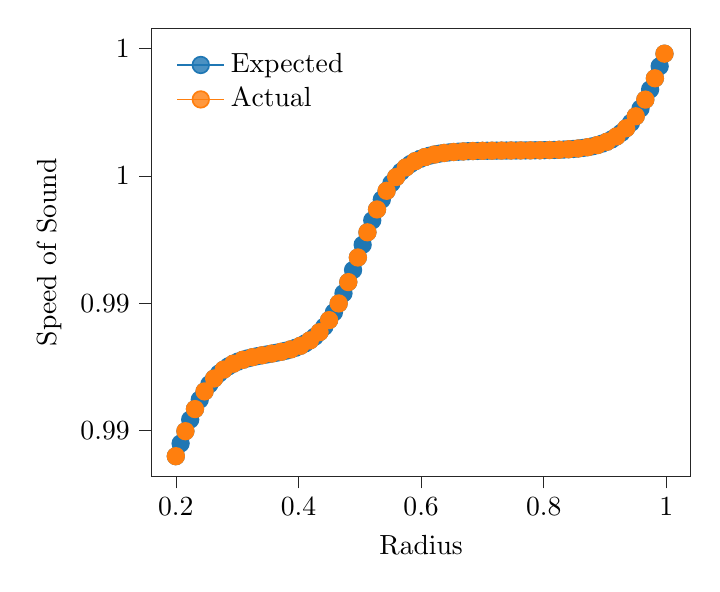
\begin{tikzpicture}

\definecolor{color0}{rgb}{0.12156862745098,0.466666666666667,0.705882352941177}
\definecolor{color1}{rgb}{1,0.498039215686275,0.0549019607843137}

\begin{axis}[
axis line style={white!15!black},
legend cell align={left},
legend style={
  fill opacity=0.8,
  draw opacity=1,
  text opacity=1,
  at={(0.03,0.97)},
  anchor=north west,
  draw=none
},
tick align=outside,
tick pos=left,
x grid style={white!80!black},
xlabel={Radius},
xmin=0.16, xmax=1.04,
xtick style={color=white!15!black},
y grid style={white!80!black},
ylabel={Speed of Sound},
ymin=0.98320056903035, ymax=1.00079997290332,
ytick style={color=white!15!black}
]
\addplot [semithick, color0, mark=*, mark size=3, mark repeat=5, mark options={solid}]
table {%
0.2 0.984000541933667
0.2015625 0.984100548886647
0.203125 0.984200432419622
0.2046875 0.984300068384446
0.20625 0.984399333875707
0.2078125 0.984498107834061
0.209375 0.984596271630271
0.2109375 0.984693709624082
0.2125 0.984790309692462
0.2140625 0.984885963722324
0.215625 0.984980568063398
0.2171875 0.985074023937652
0.21875 0.985166237802302
0.2203125 0.985257121664242
0.221875 0.985346593344428
0.2234375 0.985434576691501
0.225 0.985521001744648
0.2265625 0.985605804846342
0.228125 0.985688928706271
0.2296875 0.985770322418282
0.23125 0.985849941432696
0.2328125 0.985927747486754
0.234375 0.986003708496322
0.2359375 0.986077798412233
0.2375 0.986149997044859
0.2390625 0.986220289860638
0.240625 0.986288667754308
0.2421875 0.986355126800626
0.24375 0.986419667989276
0.2453125 0.986482296946548
0.246875 0.986543023647233
0.2484375 0.986601862119971
0.25 0.986658830149088
0.2515625 0.986713948975696
0.253125 0.98676724300061
0.2546875 0.98681873949133
0.25625 0.986868468295113
0.2578125 0.986916461559873
0.259375 0.986962753464396
0.2609375 0.987007379959106
0.2625 0.987050378518398
0.2640625 0.987091787905317
0.265625 0.987131647949157
0.2671875 0.987169999336396
0.26875 0.98720688341517
0.2703125 0.987242342013376
0.271875 0.987276417270339
0.2734375 0.987309151481869
0.275 0.987340586958444
0.2765625 0.987370765896143
0.278125 0.987399730259926
0.2796875 0.987427521678759
0.28125 0.987454181352077
0.2828125 0.987479749967015
0.284375 0.987504267625839
0.2859375 0.987527773782981
0.2875 0.987550307191088
0.2890625 0.987571905855486
0.290625 0.987592606996474
0.2921875 0.987612447018872
0.29375 0.987631461488276
0.2953125 0.987649685113462
0.296875 0.987667151734442
0.2984375 0.987683894315661
0.3 0.987699944943884
0.3015625 0.987715334830319
0.303125 0.987730094316565
0.3046875 0.987744252883996
0.30625 0.987757839166223
0.3078125 0.987770880964282
0.309375 0.987783405264264
0.3109375 0.987795438257075
0.3125 0.987807005360076
0.3140625 0.987818131240364
0.315625 0.987828839839472
0.3171875 0.987839154399291
0.31875 0.98784909748904
0.3203125 0.987858691033117
0.321875 0.9878679563397
0.3234375 0.987876914129958
0.325 0.987885584567766
0.3265625 0.987893987289837
0.328125 0.98790214143616
0.3296875 0.987910065680699
0.33125 0.987917778262275
0.3328125 0.987925297015572
0.334375 0.987932639402246
0.3359375 0.987939822542074
0.3375 0.987946863244137
0.3390625 0.987953778037998
0.340625 0.987960583204877
0.3421875 0.987967294808789
0.34375 0.98797392872766
0.3453125 0.987980500684408
0.346875 0.987987026277992
0.3484375 0.987993521014427
0.35 0.988000000337782
0.3515625 0.988006479661155
0.353125 0.988012974397646
0.3546875 0.988019499991323
0.35625 0.988026071948201
0.3578125 0.988032705867241
0.359375 0.988039417471358
0.3609375 0.988046222638482
0.3625 0.988053137432628
0.3640625 0.988060178135015
0.365625 0.988067361275209
0.3671875 0.98807470366229
0.36875 0.988082222416037
0.3703125 0.988089934998106
0.371875 0.988097859243185
0.3734375 0.988106013390094
0.375 0.988114416112798
0.3765625 0.988123086551289
0.378125 0.988132044342281
0.3796875 0.988141309649652
0.38125 0.988150903194572
0.3828125 0.98816084628522
0.384375 0.988171160845998
0.3859375 0.988181869446127
0.3875 0.9881929953275
0.3890625 0.988204562431654
0.390625 0.988216595425687
0.3921875 0.988229119726965
0.39375 0.988242161526395
0.3953125 0.988255747810073
0.396875 0.988269906379039
0.3984375 0.988284665866907
0.4 0.988300055755055
0.4015625 0.988316106385087
0.403125 0.988332848968214
0.4046875 0.988350315591207
0.40625 0.988368539218517
0.4078125 0.988387553690159
0.409375 0.988407393714916
0.4109375 0.988428094858389
0.4125 0.988449693525406
0.4140625 0.988472226936272
0.415625 0.988495733096318
0.4171875 0.988520250758199
0.41875 0.988545819376356
0.4203125 0.988572479053063
0.421875 0.988600270475462
0.4234375 0.988629234842998
0.425 0.988659413784646
0.4265625 0.988690849265375
0.428125 0.988723583481276
0.4296875 0.988757658742837
0.43125 0.98879311734588
0.4328125 0.988830001429742
0.434375 0.988868352822332
0.4359375 0.9889082128718
0.4375 0.988949622264638
0.4390625 0.988992620830155
0.440625 0.989037247331411
0.4421875 0.989083539242818
0.44375 0.989131532514817
0.4453125 0.989181261326212
0.446875 0.989232757824935
0.4484375 0.989286051858266
0.45 0.989341170693724
0.4515625 0.989398138732145
0.453125 0.989456977214666
0.4546875 0.989517703925637
0.45625 0.989580332893724
0.4578125 0.989644874093744
0.459375 0.989711333152017
0.4609375 0.989779711058255
0.4625 0.989850003887249
0.4640625 0.989922202533768
0.465625 0.989996292464284
0.4671875 0.990072253489208
0.46875 0.99015005955941
0.4703125 0.990229678590797
0.471875 0.990311072320652
0.4734375 0.99039419619934
0.475 0.990478999320756
0.4765625 0.990565424394636
0.478125 0.990653407763507
0.4796875 0.990742879466609
0.48125 0.99083376335264
0.4828125 0.990925977242617
0.484375 0.991019433143496
0.4859375 0.991114037512562
0.4875 0.991209691571851
0.4890625 0.991306291671168
0.490625 0.991403729697502
0.4921875 0.991501893527903
0.49375 0.991600667522201
0.4953125 0.99169993305125
0.496875 0.991799569055799
0.4984375 0.991899452630537
0.5 0.991999459627421
0.5015625 0.992099465272067
0.503125 0.99219934478671
0.5046875 0.992298974013166
0.50625 0.992398230029186
0.5078125 0.992496991751752
0.509375 0.992595140521059
0.5109375 0.992692560659307
0.5125 0.992789139998857
0.5140625 0.99288477037483
0.515625 0.992979348077864
0.5171875 0.99307277426338
0.51875 0.993164955314424
0.5203125 0.993255803155917
0.521875 0.993345235518834
0.5234375 0.993433176153603
0.525 0.993519554992716
0.5265625 0.993604308263212
0.528125 0.993687378550314
0.5296875 0.993768714814062
0.53125 0.993848272361297
0.5328125 0.993926012775751
0.534375 0.994001903809366
0.5359375 0.99407591923823
0.5375 0.994148038686721
0.5390625 0.99421824742356
0.540625 0.994286536133559
0.5421875 0.994352900668823
0.54375 0.994417341783093
0.5453125 0.994479864852854
0.546875 0.994540479588594
0.5484375 0.994599199739509
0.55 0.994656042794637
0.5515625 0.994711029683234
0.553125 0.994764184476907
0.5546875 0.994815534095789
0.55625 0.994865108020749
0.5578125 0.99491293801338
0.559375 0.99495905784526
0.5609375 0.995003503037712
0.5625 0.995046310613072
0.5640625 0.995087518858254
0.565625 0.995127167101171
0.5671875 0.995165295500434
0.56875 0.99520194484852
0.5703125 0.995237156388507
0.571875 0.995270971644298
0.5734375 0.995303432264168
0.575 0.995334579877347
0.5765625 0.995364455963282
0.578125 0.995393101733155
0.5796875 0.995420558023162
0.58125 0.995446865199025
0.5828125 0.995472063071189
0.584375 0.9954961908201
0.5859375 0.995519286930997
0.5875 0.995541389137587
0.5890625 0.995562534374025
0.590625 0.995582758734604
0.5921875 0.995602097440566
0.59375 0.995620584813474
0.5953125 0.995638254254612
0.596875 0.995655138229866
0.5984375 0.995671268259608
0.6 0.995686674913096
0.6015625 0.995701387806942
0.603125 0.995715435607232
0.6046875 0.995728846034892
0.60625 0.99574164587393
0.6078125 0.995753860982223
0.609375 0.995765516304507
0.6109375 0.995776635887292
0.6125 0.995787242895424
0.6140625 0.995797359630043
0.615625 0.995807007547711
0.6171875 0.995816207280501
0.61875 0.995824978656858
0.6203125 0.995833340723064
0.621875 0.995841311765143
0.6234375 0.995848909331092
0.625 0.995856150253272
0.6265625 0.995863050670899
0.628125 0.995869626052497
0.6296875 0.99587589121825
0.63125 0.995881860362164
0.6328125 0.995887547073985
0.634375 0.995892964360806
0.6359375 0.995898124668321
0.6375 0.995903039901678
0.6390625 0.995907721445908
0.640625 0.995912180185882
0.6421875 0.995916426525794
0.64375 0.995920470408134
0.6453125 0.995924321332153
0.646875 0.995927988371789
0.6484375 0.995931480193072
0.65 0.995934805070983
0.6515625 0.995937970905779
0.653125 0.99594098523878
0.6546875 0.995943855267619
0.65625 0.995946587860976
0.6578125 0.995949189572774
0.659375 0.995951666655872
0.6609375 0.995954025075258
0.6625 0.99595627052074
0.6640625 0.995958408419154
0.665625 0.995960443946116
0.6671875 0.995962382037296
0.66875 0.995964227399259
0.6703125 0.995965984519872
0.671875 0.995967657678284
0.6734375 0.995969250954509
0.675 0.995970768238611
0.6765625 0.995972213239507
0.678125 0.995973589493407
0.6796875 0.995974900371901
0.68125 0.995976149089699
0.6828125 0.995977338712054
0.684375 0.995978472161855
0.6859375 0.995979552226434
0.6875 0.995980581564065
0.6890625 0.995981562710198
0.690625 0.995982498083416
0.6921875 0.995983389991139
0.69375 0.995984240635083
0.6953125 0.995985052116483
0.696875 0.995985826441091
0.6984375 0.99598656552396
0.7 0.995987271194022
0.7015625 0.995987945198473
0.703125 0.995988589206969
0.7046875 0.995989204815643
0.70625 0.995989793550959
0.7078125 0.995990356873398
0.709375 0.995990896180996
0.7109375 0.99599141281273
0.7125 0.99599190805178
0.7140625 0.99599238312864
0.715625 0.995992839224128
0.7171875 0.995993277472259
0.71875 0.995993698963021
0.7203125 0.99599410474504
0.721875 0.99599449582815
0.7234375 0.995994873185871
0.725 0.995995237757798
0.7265625 0.995995590451909
0.728125 0.995995932146805
0.7296875 0.995996263693868
0.73125 0.995996585919359
0.7328125 0.995996899626465
0.734375 0.995997205597271
0.7359375 0.9959975045947
0.7375 0.995997797364393
0.7390625 0.995998084636562
0.740625 0.995998367127788
0.7421875 0.995998645542801
0.74375 0.995998920576223
0.7453125 0.995999192914293
0.746875 0.995999463236562
0.7484375 0.995999732217585
0.75 0.996000000528589
0.7515625 0.996000268839138
0.753125 0.996000537818796
0.7546875 0.996000808138787
0.75625 0.996001080473659
0.7578125 0.996001355502957
0.759375 0.996001633912908
0.7609375 0.996001916398121
0.7625 0.996002203663312
0.7640625 0.996002496425045
0.765625 0.996002795413511
0.7671875 0.996003101374329
0.76875 0.996003415070396
0.7703125 0.996003737283773
0.771875 0.996004068817611
0.7734375 0.996004410498143
0.775 0.996004763176713
0.7765625 0.996005127731883
0.778125 0.996005505071589
0.7796875 0.996005896135382
0.78125 0.996006301896732
0.7828125 0.996006723365422
0.784375 0.996007161590024
0.7859375 0.996007617660467
0.7875 0.996008092710702
0.7890625 0.996008587921481
0.790625 0.996009104523228
0.7921875 0.996009643799046
0.79375 0.996010207087836
0.7953125 0.996010795787547
0.796875 0.996011411358571
0.7984375 0.996012055327279
0.8 0.996012729289704
0.8015625 0.996013434915398
0.803125 0.996014173951444
0.8046875 0.996014948226658
0.80625 0.99601575965597
0.8078125 0.996016610245002
0.809375 0.99601750209485
0.8109375 0.996018437407087
0.8125 0.996019418488979
0.8140625 0.99602044775895
0.815625 0.996021527752279
0.8171875 0.996022661127064
0.81875 0.996023850670446
0.8203125 0.996025099305121
0.821875 0.99602641009613
0.8234375 0.996027786257968
0.825 0.996029231161992
0.8265625 0.996030748344171
0.828125 0.996032341513167
0.8296875 0.996034014558775
0.83125 0.996035771560727
0.8328125 0.996037616797878
0.834375 0.996039554757779
0.8359375 0.996041590146669
0.8375 0.996043727899874
0.8390625 0.996045973192643
0.840625 0.996048331451433
0.8421875 0.996050808365651
0.84375 0.99605340989986
0.8453125 0.996056142306476
0.846875 0.996059012138958
0.8484375 0.99606202626549
0.85 0.996065191883192
0.8515625 0.996068516532841
0.853125 0.996072008114122
0.8546875 0.996075674901416
0.85625 0.996079525560123
0.8578125 0.996083569163517
0.859375 0.996087815210152
0.8609375 0.996092273641784
0.8625 0.996096954861836
0.8640625 0.996101869754369
0.865625 0.996107029703561
0.8671875 0.996112446613664
0.86875 0.99611813292943
0.8703125 0.996124101656964
0.871875 0.996130366384967
0.8734375 0.996136941306354
0.875 0.996143841240155
0.8765625 0.996151081653687
0.878125 0.996158678684891
0.8796875 0.996166649164795
0.88125 0.996175010639986
0.8828125 0.996183781395013
0.884375 0.996192980474604
0.8859375 0.99620262770557
0.8875 0.996212743718267
0.8890625 0.996223349967452
0.890625 0.996234468752366
0.8921875 0.996246123235863
0.89375 0.996258337462352
0.8953125 0.996271136374368
0.896875 0.996284545827466
0.8984375 0.99629859260322
0.9 0.996313304419992
0.9015625 0.996328709941177
0.903125 0.996344838780554
0.9046875 0.996361721504406
0.90625 0.996379389629974
0.9078125 0.996397875619856
0.909375 0.996417212871876
0.9109375 0.996437435703965
0.9125 0.99645857933354
0.9140625 0.996480679850876
0.915625 0.996503774185906
0.9171875 0.996527900067896
0.91875 0.996553095977414
0.9203125 0.996579401090003
0.921875 0.996606855210946
0.9234375 0.996635498700543
0.925 0.996665372389287
0.9265625 0.996696517482366
0.928125 0.996728975452927
0.9296875 0.996762787923574
0.93125 0.996797996535619
0.9328125 0.996834642805644
0.934375 0.99687276796903
0.9359375 0.996912412810164
0.9375 0.996953617479149
0.9390625 0.996996421294959
0.940625 0.997040862535105
0.9421875 0.997086978212043
0.94375 0.997134803836707
0.9453125 0.997184373169752
0.946875 0.997235717961291
0.9484375 0.997288867680121
0.95 0.997343849233688
0.9515625 0.99740068668026
0.953125 0.997459400935069
0.9546875 0.997520009472411
0.95625 0.997582526025983
0.9578125 0.997646960289984
0.959375 0.997713317623768
0.9609375 0.997781598763074
0.9625 0.997851799541075
0.9640625 0.997923910622686
0.965625 0.99799791725571
0.9671875 0.998073799042532
0.96875 0.998151529736121
0.9703125 0.998231077064117
0.971875 0.998312402584702
0.9734375 0.998395461577857
0.975 0.998480202975387
0.9765625 0.998566569332831
0.978125 0.998654496846022
0.9796875 0.998743915414651
0.98125 0.998834748754659
0.9828125 0.998926914560766
0.984375 0.999020324719782
0.9859375 0.99911488557469
0.9875 0.99921049823879
0.9890625 0.999307058958444
0.990625 0.999404459522227
0.9921875 0.999502587713568
0.99375 0.999601327803226
0.9953125 0.999700561077321
0.996875 0.999800166395987
0.9984375 0.999900020777216
1 1
};
\addlegendentry{Expected}
\addplot [semithick, color1, mark=*, mark size=3, mark repeat=10, mark options={solid}]
table {%
0.2 0.984000542019354
0.2015625 0.984100538570465
0.203125 0.984200411755927
0.2046875 0.984300037478986
0.20625 0.984399292884513
0.2078125 0.984498056961819
0.209375 0.984596211128208
0.2109375 0.98469363978739
0.2125 0.984790230857325
0.2140625 0.984885876262573
0.215625 0.98498047238688
0.2171875 0.985073920482345
0.21875 0.985166127032258
0.2203125 0.985257004065404
0.221875 0.985346469420391
0.2234375 0.985434446959279
0.225 0.98552086673049
0.2265625 0.985605665081666
0.228125 0.985688784723747
0.2296875 0.985770174748117
0.23125 0.985849790599148
0.2328125 0.985927594004909
0.234375 0.986003552869154
0.2359375 0.986077641127965
0.2375 0.986149838574637
0.2390625 0.986220130656513
0.240625 0.986288508247539
0.2421875 0.986354967400289
0.24375 0.986419509081172
0.2453125 0.986482138892399
0.246875 0.986542866784147
0.2484375 0.98660170676016
0.25 0.986658676579815
0.2515625 0.986713797459438
0.253125 0.986767093775402
0.2546875 0.986818592771284
0.25625 0.986868324271075
0.2578125 0.98691632040021
0.259375 0.986962615315875
0.2609375 0.987007244947868
0.2625 0.987050246750991
0.2640625 0.987091659469774
0.265625 0.987131522916112
0.2671875 0.987169877760217
0.26875 0.987206765335094
0.2703125 0.987242227454642
0.271875 0.987276306245304
0.2734375 0.987309043991106
0.275 0.987340482991801
0.2765625 0.987370665433774
0.278125 0.987399633273278
0.2796875 0.987427428131517
0.28125 0.987454091201058
0.2828125 0.987479663163019
0.284375 0.987504184114449
0.2859375 0.987527693505313
0.2875 0.98755023008449
0.2890625 0.987571831854191
0.290625 0.9875925360322
0.2921875 0.987612379021383
0.29375 0.987631396385893
0.2953125 0.987649622833532
0.296875 0.987667092203763
0.2984375 0.987683837460875
0.3 0.987699890691827
0.3015625 0.987715283108339
0.303125 0.987730045052807
0.3046875 0.987744206007658
0.30625 0.987757794607782
0.3078125 0.987770838655695
0.309375 0.987783365139148
0.3109375 0.98779540025086
0.3125 0.987806969410141
0.3140625 0.987818097286156
0.315625 0.987828807822605
0.3171875 0.987839124263634
0.31875 0.98784906918079
0.3203125 0.987858664500862
0.321875 0.987867931534466
0.3234375 0.987876891005252
0.325 0.987885563079613
0.3265625 0.987893967396799
0.328125 0.987902123099364
0.3296875 0.987910048863849
0.33125 0.987917762931659
0.3328125 0.987925283140076
0.334375 0.987932626953352
0.3359375 0.987939811493866
0.3375 0.987946853573297
0.3390625 0.987953769723811
0.340625 0.98796057622922
0.3421875 0.987967289156136
0.34375 0.987973924385075
0.3453125 0.987980497641544
0.346875 0.987987024527085
0.3484375 0.987993520550299
0.35 0.988000001157834
0.3515625 0.988006481765371
0.353125 0.98801297778859
0.3546875 0.988019504674139
0.35625 0.988026077930618
0.3578125 0.988032713159569
0.359375 0.988039426086497
0.3609375 0.988046232591919
0.3625 0.988053148742442
0.3640625 0.98806019082188
0.365625 0.988067375362393
0.3671875 0.988074719175661
0.36875 0.988082239384058
0.3703125 0.988089953451836
0.371875 0.988097879216269
0.3734375 0.988106034918762
0.375 0.988114439235851
0.3765625 0.988123111310083
0.378125 0.988132070780705
0.3796875 0.988141337814104
0.38125 0.988150933133922
0.3828125 0.988160878050769
0.384375 0.988171194491426
0.3859375 0.988181905027431
0.3875 0.988193032902921
0.3890625 0.988204602061585
0.390625 0.988216637172577
0.3921875 0.988229163655196
0.39375 0.988242207702146
0.3953125 0.988255796301162
0.396875 0.988269957254748
0.3984375 0.988284719197773
0.4 0.988300111612648
0.4015625 0.988316164841748
0.403125 0.98833291009677
0.4046875 0.988350379464653
0.40625 0.988368605909658
0.4078125 0.988387623271224
0.409375 0.988407466257124
0.4109375 0.988428170431479
0.4125 0.988449772197124
0.4140625 0.988472308771811
0.415625 0.988495818157714
0.4171875 0.988520339103674
0.41875 0.988545911059617
0.4203125 0.988572574122552
0.421875 0.988600368973554
0.4234375 0.988629336805148
0.425 0.988659519238492
0.4265625 0.988690958229793
0.428125 0.988723695965391
0.4296875 0.988757774744993
0.43125 0.988793236852577
0.4328125 0.988830124414544
0.434375 0.988868479244747
0.4359375 0.988908342676152
0.4375 0.988949755378929
0.4390625 0.98899275716494
0.440625 0.989037386778686
0.4421875 0.989083681674941
0.44375 0.989131677783485
0.4453125 0.989181409261496
0.446875 0.989232908234404
0.4484375 0.989286204526211
0.45 0.989341325380513
0.4515625 0.989398295173717
0.453125 0.989457135122194
0.4546875 0.989517862985384
0.45625 0.989580492767111
0.4578125 0.989645034417647
0.459375 0.989711493539319
0.4609375 0.98977987109867
0.4625 0.989850163148432
0.4640625 0.989922360562726
0.465625 0.989996448789093
0.4671875 0.990072407621048
0.46875 0.990150210994911
0.4703125 0.990229826814696
0.471875 0.990311216808754
0.4734375 0.990394336421754
0.475 0.990479134745392
0.4765625 0.990565554490936
0.478125 0.990653532006369
0.4796875 0.990742997340459
0.48125 0.99083387435562
0.4828125 0.990926080890818
0.484375 0.991019528975192
0.4859375 0.991114125092381
0.4875 0.991209770494826
0.4890625 0.991306361566602
0.490625 0.991403790232585
0.4921875 0.991501944411025
0.49375 0.991600708505906
0.4953125 0.991699963934777
0.496875 0.991799589687169
0.4984375 0.991899462908144
0.5 0.991999459501105
0.5015625 0.992099454743644
0.503125 0.992199323909957
0.5046875 0.992298942893246
0.50625 0.992398188821544
0.5078125 0.992496940660486
0.509375 0.992595079796797
0.5109375 0.99269249059664
0.5125 0.992789060933354
0.5140625 0.992884682679702
0.515625 0.992979252160325
0.5171875 0.993072670560762
0.51875 0.993164844290118
0.5203125 0.993255685295191
0.521875 0.99334511132459
0.5234375 0.99343304614214
0.525 0.99351941968955
0.5265625 0.993604168199006
0.528125 0.993687234256956
0.5296875 0.993768566820951
0.53125 0.993848121191855
0.5328125 0.993925858944195
0.534375 0.99400174781777
0.5359375 0.994075761573883
0.5375 0.994147879819793
0.5390625 0.994218087805088
0.540625 0.994286376193745
0.5421875 0.99435274081564
0.54375 0.994417182401192
0.5453125 0.994479706302753
0.546875 0.994540322206146
0.5484375 0.99459904383561
0.55 0.994655888655176
0.5515625 0.994710877569247
0.553125 0.994764034624923
0.5546875 0.994815386718341
0.55625 0.994864963307029
0.5578125 0.994912796130018
0.559375 0.994958918937205
0.5609375 0.995003367229198
0.5625 0.995046178008647
0.5640625 0.995087389543851
0.565625 0.995127041145225
0.5671875 0.995165172955
0.56875 0.99520182575041
0.5703125 0.995237040760414
0.571875 0.995270859495909
0.5734375 0.995303323593251
0.575 0.995334474670805
0.5765625 0.995364354198178
0.578125 0.995393003377691
0.5796875 0.995420463037613
0.58125 0.995446773536632
0.5828125 0.995471974678994
0.584375 0.995496105639743
0.5859375 0.99551920489945
0.5875 0.99554131018785
0.5890625 0.995562458435763
0.590625 0.995582685734742
0.5921875 0.995602027303832
0.59375 0.995620517462904
0.5953125 0.995638189612002
0.596875 0.99565507621619
0.5984375 0.99567120879539
0.6 0.99568661791875
0.6015625 0.995701333203077
0.603125 0.995715383314918
0.6046875 0.995728795975899
0.60625 0.995741597970942
0.6078125 0.995753815159019
0.609375 0.995765472486118
0.6109375 0.995776594000141
0.6125 0.995787202867441
0.6140625 0.995797321390759
0.615625 0.995806971028341
0.6171875 0.995816172414004
0.61875 0.995824945377991
0.6203125 0.995833308968413
0.621875 0.995841281473156
0.6234375 0.995848880442084
0.625 0.995856122709439
0.6265625 0.995863024416314
0.628125 0.995869601033097
0.6296875 0.995875867381824
0.63125 0.995881837658331
0.6328125 0.995887525454166
0.634375 0.995892943778198
0.6359375 0.995898105077859
0.6375 0.995903021260004
0.6390625 0.995907703711326
0.640625 0.995912163318324
0.6421875 0.995916410486774
0.64375 0.995920455160706
0.6453125 0.995924306840866
0.646875 0.995927974602643
0.6484375 0.995931467113475
0.65 0.995934792649703
0.6515625 0.9959379591129
0.653125 0.995940974045658
0.6546875 0.995943844646839
0.65625 0.995946577786306
0.6578125 0.995949180019123
0.659375 0.99595165759925
0.6609375 0.995954016492733
0.6625 0.995956262390396
0.6640625 0.995958400720057
0.665625 0.995960436658271
0.6671875 0.99596237514161
0.66875 0.995964220877508
0.6703125 0.995965978354663
0.671875 0.995967651853024
0.6734375 0.99596924545337
0.675 0.995970763046498
0.6765625 0.99597220834203
0.678125 0.995973584876848
0.6796875 0.995974896023187
0.68125 0.995976144996378
0.6828125 0.995977334862262
0.684375 0.995978468544298
0.6859375 0.995979548830358
0.6875 0.995980578379236
0.6890625 0.995981559726879
0.690625 0.995982495292344
0.6921875 0.995983387383507
0.69375 0.995984238202519
0.6953125 0.995985049851032
0.696875 0.995985824335194
0.6984375 0.995986563570442
0.7 0.995987269386074
0.7015625 0.995987943529633
0.703125 0.995988587671111
0.7046875 0.995989203406963
0.70625 0.99598979226396
0.7078125 0.995990355702877
0.709375 0.995990895122031
0.7109375 0.995991411860674
0.7125 0.995991907202242
0.7140625 0.995992382377482
0.715625 0.99599283856745
0.7171875 0.995993276906392
0.71875 0.99599369848452
0.7203125 0.995994104350672
0.721875 0.99599449551489
0.7234375 0.995994872950893
0.725 0.995995237598466
0.7265625 0.995995590365778
0.728125 0.995995932131606
0.7296875 0.995996263747507
0.73125 0.995996586039915
0.7328125 0.995996899812179
0.734375 0.995997205846547
0.7359375 0.995997504906098
0.7375 0.995997797736628
0.7390625 0.995998085068498
0.740625 0.995998367618437
0.7421875 0.995998646091321
0.74375 0.995998921181916
0.7453125 0.995999193576601
0.746875 0.99599946395507
0.7484375 0.995999732992015
0.75 0.996000001358802
0.7515625 0.996000269725134
0.753125 0.996000538760714
0.7546875 0.996000809136904
0.75625 0.996001081528391
0.7578125 0.99600135661486
0.759375 0.99600163508268
0.7609375 0.996001917626605
0.7625 0.996002204951495
0.7640625 0.996002497774063
0.765625 0.996002796824648
0.7671875 0.996003102849025
0.76875 0.996003416610248
0.7703125 0.996003738890537
0.771875 0.996004070493211
0.7734375 0.99600441224467
0.775 0.996004764996435
0.7765625 0.996005129627247
0.778125 0.996005507045229
0.7796875 0.996005898190124
0.78125 0.996006304035602
0.7828125 0.996006725591651
0.784375 0.996007163907057
0.7859375 0.996007620071971
0.7875 0.996008095220578
0.7890625 0.996008590533865
0.790625 0.99600910724251
0.7921875 0.996009646629875
0.79375 0.99601021003513
0.7953125 0.996010798856509
0.796875 0.996011414554698
0.7984375 0.996012058656374
0.8 0.996012732757891
0.8015625 0.996013438529137
0.803125 0.996014177717544
0.8046875 0.996014952152294
0.80625 0.996015763748697
0.8078125 0.996016614512774
0.809375 0.996017506546037
0.8109375 0.996018442050494
0.8125 0.996019423333868
0.8140625 0.996020452815054
0.815625 0.996021533029831
0.8171875 0.996022666636814
0.81875 0.996023856423687
0.8203125 0.996025105313711
0.821875 0.996026416372521
0.8234375 0.996027792815226
0.825 0.996029238013831
0.8265625 0.996030755504977
0.828125 0.99603234899803
0.8296875 0.996034022383518
0.83125 0.996035779741937
0.8328125 0.996037625352941
0.834375 0.996039563704913
0.8359375 0.996041599504958
0.8375 0.996043737689303
0.8390625 0.99604598343414
0.840625 0.996048342166902
0.8421875 0.996050819578012
0.84375 0.996053421633092
0.8453125 0.996056154585657
0.846875 0.996059024990304
0.8484375 0.996062039716402
0.85 0.996065205962296
0.8515625 0.996068531270032
0.853125 0.996072023540612
0.8546875 0.996075691049775
0.85625 0.996079542464325
0.8578125 0.996083586858985
0.859375 0.996087833733802
0.8609375 0.996092293032069
0.8625 0.996096975158789
0.8640625 0.996101890999645
0.865625 0.996107051940475
0.8671875 0.996112469887234
0.86875 0.996118157286407
0.8703125 0.996124127145869
0.871875 0.99613039305612
0.8734375 0.996136969211897
0.875 0.996143870434077
0.8765625 0.996151112191834
0.878125 0.996158710624979
0.8796875 0.996166682566409
0.88125 0.996175045564575
0.8828125 0.996183817905873
0.884375 0.996193018636852
0.8859375 0.996202667586109
0.8875 0.996212785385732
0.8890625 0.996223393492147
0.890625 0.996234514206185
0.8921875 0.996246170692186
0.89375 0.996258386995937
0.8953125 0.996271188061206
0.896875 0.996284599744623
0.8984375 0.996298648828654
0.9 0.996313363032339
0.9015625 0.996328771019508
0.903125 0.99634490240411
0.9046875 0.996361787752286
0.90625 0.996379458580801
0.9078125 0.996397947351397
0.909375 0.996417287460625
0.9109375 0.996437513224683
0.9125 0.996458659858756
0.9140625 0.996480763450336
0.915625 0.996503860925981
0.9171875 0.996527990010936
0.91875 0.996553189181057
0.9203125 0.996579497606432
0.921875 0.996606955086097
0.9234375 0.996635601973261
0.925 0.996665479090439
0.9265625 0.9966966276339
0.928125 0.996729089066892
0.9296875 0.9967629050011
0.93125 0.996798117065855
0.9328125 0.996834766764676
0.934375 0.996872895318767
0.9359375 0.996912543497216
0.9375 0.996953751433694
0.9390625 0.996996558429622
0.940625 0.997041002743852
0.9421875 0.997087121369108
0.94375 0.997134949795571
0.9453125 0.997184521762187
0.946875 0.997235868996483
0.9484375 0.997289020943902
0.95 0.997344004487888
0.9515625 0.997400843662211
0.953125 0.997459559357272
0.9546875 0.997520169022392
0.95625 0.997582686366363
0.9578125 0.997647121058781
0.959375 0.997713478434953
0.9609375 0.997781759207394
0.9625 0.997851959187171
0.9640625 0.997924069018498
0.965625 0.997998073930204
0.9671875 0.998073953507733
0.96875 0.998151681489463
0.9703125 0.998231225591102
0.971875 0.99831254736186
0.9734375 0.998395602075987
0.975 0.998480338663054
0.9765625 0.998566699680098
0.978125 0.998654621328378
0.9796875 0.998744033517082
0.98125 0.998834859975838
0.9828125 0.998927018417289
0.984375 0.999020420750399
0.9859375 0.999114973344484
0.9875 0.999210577343224
0.9890625 0.999307129027227
0.990625 0.999404520222934
0.9921875 0.999502638754955
0.99375 0.999601368938184
0.9953125 0.999700592105417
0.996875 0.999800187165552
0.9984375 0.999900031186939
1 1
};
\addlegendentry{Actual}
\end{axis}

\end{tikzpicture}

    \end{center}
\end{figure}

\begin{figure}
    \begin{center}
        % This file was created with tikzplotlib v0.9.12.
\begin{tikzpicture}

\definecolor{color0}{rgb}{0.12156862745098,0.466666666666667,0.705882352941177}

\begin{groupplot}[group style={group size=1 by 2}]
\nextgroupplot[
axis line style={white!15!black},
legend cell align={left},
legend style={fill opacity=0.8, draw opacity=1, text opacity=1, draw=none},
log basis y={10},
scaled x ticks=manual:{}{\pgfmathparse{#1}},
tick align=outside,
tick pos=left,
title={Rate Of Convergence},
x grid style={white!80!black},
xmin=0.49602339181245, xmax=0.60495126705655,
xtick style={color=white!15!black},
xticklabels={},
y grid style={white!80!black},
ymin=1.93465772282466, ymax=2.50490389113768,
ymode=log,
ytick style={color=white!15!black}
]
\addplot [semithick, color0]
table {%
0.6 2.220755792495
0.555555555556 2.163324274032
0.529411764706 2.475663773488
0.515151515152 1.957508006467
0.507692307692 1.997639457419
0.503875968992 1.996551880759
0.501945525292 1.997726606828
0.500974658869 1.998727064418
};
\addlegendentry{Speed Of Sound}

\nextgroupplot[
axis line style={white!15!black},
legend cell align={left},
legend style={fill opacity=0.8, draw opacity=1, text opacity=1, draw=none},
log basis y={10},
tick align=outside,
tick pos=left,
x grid style={white!80!black},
xlabel={Del r},
xmin=0.49602339181245, xmax=0.60495126705655,
xtick style={color=white!15!black},
y grid style={white!80!black},
ymin=0.362953235346687, ymax=0.506191289267272,
ymode=log,
ytick style={color=white!15!black}
]
\addplot [semithick, color0]
table {%
0.6 0.368482797082
0.555555555556 0.423998453276
0.529411764706 0.458768919907
0.515151515152 0.478465639055
0.507692307692 0.488986846835
0.503875968992 0.494429721197
0.501945525292 0.497198646885
0.500974658869 0.498595233207
};
\addlegendentry{LEE}
\end{groupplot}

\end{tikzpicture}

    \end{center}
\end{figure}

\begin{figure}
    \begin{center}
        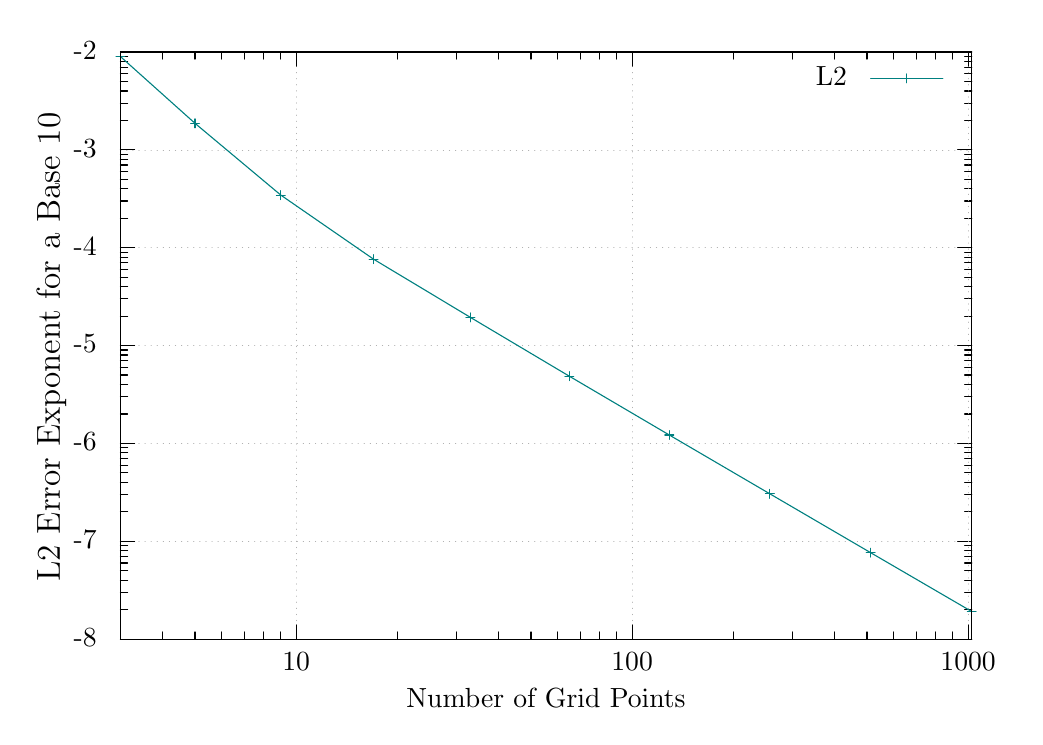
\begin{tikzpicture}[gnuplot]
%% generated with GNUPLOT 5.2p8 (Lua 5.3; terminal rev. Nov 2018, script rev. 108)
%% Tue 21 Sep 2021 05:01:33 PM EDT
\path (0.000,0.000) rectangle (12.500,8.750);
\gpcolor{color=gp lt color axes}
\gpsetlinetype{gp lt axes}
\gpsetdashtype{gp dt axes}
\gpsetlinewidth{0.50}
\draw[gp path] (1.136,0.985)--(11.947,0.985);
\gpcolor{color=gp lt color border}
\gpsetlinetype{gp lt border}
\gpsetdashtype{gp dt solid}
\gpsetlinewidth{1.00}
\draw[gp path] (1.136,0.985)--(1.316,0.985);
\draw[gp path] (11.947,0.985)--(11.767,0.985);
\node[gp node right] at (0.952,0.985) {{-8}};
\draw[gp path] (1.136,1.359)--(1.226,1.359);
\draw[gp path] (11.947,1.359)--(11.857,1.359);
\draw[gp path] (1.136,1.578)--(1.226,1.578);
\draw[gp path] (11.947,1.578)--(11.857,1.578);
\draw[gp path] (1.136,1.733)--(1.226,1.733);
\draw[gp path] (11.947,1.733)--(11.857,1.733);
\draw[gp path] (1.136,1.854)--(1.226,1.854);
\draw[gp path] (11.947,1.854)--(11.857,1.854);
\draw[gp path] (1.136,1.952)--(1.226,1.952);
\draw[gp path] (11.947,1.952)--(11.857,1.952);
\draw[gp path] (1.136,2.035)--(1.226,2.035);
\draw[gp path] (11.947,2.035)--(11.857,2.035);
\draw[gp path] (1.136,2.107)--(1.226,2.107);
\draw[gp path] (11.947,2.107)--(11.857,2.107);
\draw[gp path] (1.136,2.171)--(1.226,2.171);
\draw[gp path] (11.947,2.171)--(11.857,2.171);
\gpcolor{color=gp lt color axes}
\gpsetlinetype{gp lt axes}
\gpsetdashtype{gp dt axes}
\gpsetlinewidth{0.50}
\draw[gp path] (1.136,2.228)--(11.947,2.228);
\gpcolor{color=gp lt color border}
\gpsetlinetype{gp lt border}
\gpsetdashtype{gp dt solid}
\gpsetlinewidth{1.00}
\draw[gp path] (1.136,2.228)--(1.316,2.228);
\draw[gp path] (11.947,2.228)--(11.767,2.228);
\node[gp node right] at (0.952,2.228) {{-7}};
\draw[gp path] (1.136,2.602)--(1.226,2.602);
\draw[gp path] (11.947,2.602)--(11.857,2.602);
\draw[gp path] (1.136,2.821)--(1.226,2.821);
\draw[gp path] (11.947,2.821)--(11.857,2.821);
\draw[gp path] (1.136,2.976)--(1.226,2.976);
\draw[gp path] (11.947,2.976)--(11.857,2.976);
\draw[gp path] (1.136,3.096)--(1.226,3.096);
\draw[gp path] (11.947,3.096)--(11.857,3.096);
\draw[gp path] (1.136,3.195)--(1.226,3.195);
\draw[gp path] (11.947,3.195)--(11.857,3.195);
\draw[gp path] (1.136,3.278)--(1.226,3.278);
\draw[gp path] (11.947,3.278)--(11.857,3.278);
\draw[gp path] (1.136,3.350)--(1.226,3.350);
\draw[gp path] (11.947,3.350)--(11.857,3.350);
\draw[gp path] (1.136,3.413)--(1.226,3.413);
\draw[gp path] (11.947,3.413)--(11.857,3.413);
\gpcolor{color=gp lt color axes}
\gpsetlinetype{gp lt axes}
\gpsetdashtype{gp dt axes}
\gpsetlinewidth{0.50}
\draw[gp path] (1.136,3.470)--(11.947,3.470);
\gpcolor{color=gp lt color border}
\gpsetlinetype{gp lt border}
\gpsetdashtype{gp dt solid}
\gpsetlinewidth{1.00}
\draw[gp path] (1.136,3.470)--(1.316,3.470);
\draw[gp path] (11.947,3.470)--(11.767,3.470);
\node[gp node right] at (0.952,3.470) {{-6}};
\draw[gp path] (1.136,3.844)--(1.226,3.844);
\draw[gp path] (11.947,3.844)--(11.857,3.844);
\draw[gp path] (1.136,4.063)--(1.226,4.063);
\draw[gp path] (11.947,4.063)--(11.857,4.063);
\draw[gp path] (1.136,4.218)--(1.226,4.218);
\draw[gp path] (11.947,4.218)--(11.857,4.218);
\draw[gp path] (1.136,4.339)--(1.226,4.339);
\draw[gp path] (11.947,4.339)--(11.857,4.339);
\draw[gp path] (1.136,4.437)--(1.226,4.437);
\draw[gp path] (11.947,4.437)--(11.857,4.437);
\draw[gp path] (1.136,4.521)--(1.226,4.521);
\draw[gp path] (11.947,4.521)--(11.857,4.521);
\draw[gp path] (1.136,4.593)--(1.226,4.593);
\draw[gp path] (11.947,4.593)--(11.857,4.593);
\draw[gp path] (1.136,4.656)--(1.226,4.656);
\draw[gp path] (11.947,4.656)--(11.857,4.656);
\gpcolor{color=gp lt color axes}
\gpsetlinetype{gp lt axes}
\gpsetdashtype{gp dt axes}
\gpsetlinewidth{0.50}
\draw[gp path] (1.136,4.713)--(11.947,4.713);
\gpcolor{color=gp lt color border}
\gpsetlinetype{gp lt border}
\gpsetdashtype{gp dt solid}
\gpsetlinewidth{1.00}
\draw[gp path] (1.136,4.713)--(1.316,4.713);
\draw[gp path] (11.947,4.713)--(11.767,4.713);
\node[gp node right] at (0.952,4.713) {{-5}};
\draw[gp path] (1.136,5.087)--(1.226,5.087);
\draw[gp path] (11.947,5.087)--(11.857,5.087);
\draw[gp path] (1.136,5.306)--(1.226,5.306);
\draw[gp path] (11.947,5.306)--(11.857,5.306);
\draw[gp path] (1.136,5.461)--(1.226,5.461);
\draw[gp path] (11.947,5.461)--(11.857,5.461);
\draw[gp path] (1.136,5.582)--(1.226,5.582);
\draw[gp path] (11.947,5.582)--(11.857,5.582);
\draw[gp path] (1.136,5.680)--(1.226,5.680);
\draw[gp path] (11.947,5.680)--(11.857,5.680);
\draw[gp path] (1.136,5.763)--(1.226,5.763);
\draw[gp path] (11.947,5.763)--(11.857,5.763);
\draw[gp path] (1.136,5.835)--(1.226,5.835);
\draw[gp path] (11.947,5.835)--(11.857,5.835);
\draw[gp path] (1.136,5.899)--(1.226,5.899);
\draw[gp path] (11.947,5.899)--(11.857,5.899);
\gpcolor{color=gp lt color axes}
\gpsetlinetype{gp lt axes}
\gpsetdashtype{gp dt axes}
\gpsetlinewidth{0.50}
\draw[gp path] (1.136,5.956)--(11.947,5.956);
\gpcolor{color=gp lt color border}
\gpsetlinetype{gp lt border}
\gpsetdashtype{gp dt solid}
\gpsetlinewidth{1.00}
\draw[gp path] (1.136,5.956)--(1.316,5.956);
\draw[gp path] (11.947,5.956)--(11.767,5.956);
\node[gp node right] at (0.952,5.956) {{-4}};
\draw[gp path] (1.136,6.330)--(1.226,6.330);
\draw[gp path] (11.947,6.330)--(11.857,6.330);
\draw[gp path] (1.136,6.549)--(1.226,6.549);
\draw[gp path] (11.947,6.549)--(11.857,6.549);
\draw[gp path] (1.136,6.704)--(1.226,6.704);
\draw[gp path] (11.947,6.704)--(11.857,6.704);
\draw[gp path] (1.136,6.824)--(1.226,6.824);
\draw[gp path] (11.947,6.824)--(11.857,6.824);
\draw[gp path] (1.136,6.923)--(1.226,6.923);
\draw[gp path] (11.947,6.923)--(11.857,6.923);
\draw[gp path] (1.136,7.006)--(1.226,7.006);
\draw[gp path] (11.947,7.006)--(11.857,7.006);
\draw[gp path] (1.136,7.078)--(1.226,7.078);
\draw[gp path] (11.947,7.078)--(11.857,7.078);
\draw[gp path] (1.136,7.141)--(1.226,7.141);
\draw[gp path] (11.947,7.141)--(11.857,7.141);
\gpcolor{color=gp lt color axes}
\gpsetlinetype{gp lt axes}
\gpsetdashtype{gp dt axes}
\gpsetlinewidth{0.50}
\draw[gp path] (1.136,7.198)--(11.947,7.198);
\gpcolor{color=gp lt color border}
\gpsetlinetype{gp lt border}
\gpsetdashtype{gp dt solid}
\gpsetlinewidth{1.00}
\draw[gp path] (1.136,7.198)--(1.316,7.198);
\draw[gp path] (11.947,7.198)--(11.767,7.198);
\node[gp node right] at (0.952,7.198) {{-3}};
\draw[gp path] (1.136,7.572)--(1.226,7.572);
\draw[gp path] (11.947,7.572)--(11.857,7.572);
\draw[gp path] (1.136,7.791)--(1.226,7.791);
\draw[gp path] (11.947,7.791)--(11.857,7.791);
\draw[gp path] (1.136,7.946)--(1.226,7.946);
\draw[gp path] (11.947,7.946)--(11.857,7.946);
\draw[gp path] (1.136,8.067)--(1.226,8.067);
\draw[gp path] (11.947,8.067)--(11.857,8.067);
\draw[gp path] (1.136,8.165)--(1.226,8.165);
\draw[gp path] (11.947,8.165)--(11.857,8.165);
\draw[gp path] (1.136,8.249)--(1.226,8.249);
\draw[gp path] (11.947,8.249)--(11.857,8.249);
\draw[gp path] (1.136,8.321)--(1.226,8.321);
\draw[gp path] (11.947,8.321)--(11.857,8.321);
\draw[gp path] (1.136,8.384)--(1.226,8.384);
\draw[gp path] (11.947,8.384)--(11.857,8.384);
\gpcolor{color=gp lt color axes}
\gpsetlinetype{gp lt axes}
\gpsetdashtype{gp dt axes}
\gpsetlinewidth{0.50}
\draw[gp path] (1.136,8.441)--(11.947,8.441);
\gpcolor{color=gp lt color border}
\gpsetlinetype{gp lt border}
\gpsetdashtype{gp dt solid}
\gpsetlinewidth{1.00}
\draw[gp path] (1.136,8.441)--(1.316,8.441);
\draw[gp path] (11.947,8.441)--(11.767,8.441);
\node[gp node right] at (0.952,8.441) {{-2}};
\draw[gp path] (1.136,0.985)--(1.136,1.075);
\draw[gp path] (1.136,8.441)--(1.136,8.351);
\draw[gp path] (1.669,0.985)--(1.669,1.075);
\draw[gp path] (1.669,8.441)--(1.669,8.351);
\draw[gp path] (2.083,0.985)--(2.083,1.075);
\draw[gp path] (2.083,8.441)--(2.083,8.351);
\draw[gp path] (2.421,0.985)--(2.421,1.075);
\draw[gp path] (2.421,8.441)--(2.421,8.351);
\draw[gp path] (2.706,0.985)--(2.706,1.075);
\draw[gp path] (2.706,8.441)--(2.706,8.351);
\draw[gp path] (2.954,0.985)--(2.954,1.075);
\draw[gp path] (2.954,8.441)--(2.954,8.351);
\draw[gp path] (3.172,0.985)--(3.172,1.075);
\draw[gp path] (3.172,8.441)--(3.172,8.351);
\gpcolor{color=gp lt color axes}
\gpsetlinetype{gp lt axes}
\gpsetdashtype{gp dt axes}
\gpsetlinewidth{0.50}
\draw[gp path] (3.367,0.985)--(3.367,8.441);
\gpcolor{color=gp lt color border}
\gpsetlinetype{gp lt border}
\gpsetdashtype{gp dt solid}
\gpsetlinewidth{1.00}
\draw[gp path] (3.367,0.985)--(3.367,1.165);
\draw[gp path] (3.367,8.441)--(3.367,8.261);
\node[gp node center] at (3.367,0.677) {$10$};
\draw[gp path] (4.652,0.985)--(4.652,1.075);
\draw[gp path] (4.652,8.441)--(4.652,8.351);
\draw[gp path] (5.403,0.985)--(5.403,1.075);
\draw[gp path] (5.403,8.441)--(5.403,8.351);
\draw[gp path] (5.936,0.985)--(5.936,1.075);
\draw[gp path] (5.936,8.441)--(5.936,8.351);
\draw[gp path] (6.350,0.985)--(6.350,1.075);
\draw[gp path] (6.350,8.441)--(6.350,8.351);
\draw[gp path] (6.688,0.985)--(6.688,1.075);
\draw[gp path] (6.688,8.441)--(6.688,8.351);
\draw[gp path] (6.973,0.985)--(6.973,1.075);
\draw[gp path] (6.973,8.441)--(6.973,8.351);
\draw[gp path] (7.221,0.985)--(7.221,1.075);
\draw[gp path] (7.221,8.441)--(7.221,8.351);
\draw[gp path] (7.439,0.985)--(7.439,1.075);
\draw[gp path] (7.439,8.441)--(7.439,8.351);
\gpcolor{color=gp lt color axes}
\gpsetlinetype{gp lt axes}
\gpsetdashtype{gp dt axes}
\gpsetlinewidth{0.50}
\draw[gp path] (7.634,0.985)--(7.634,8.441);
\gpcolor{color=gp lt color border}
\gpsetlinetype{gp lt border}
\gpsetdashtype{gp dt solid}
\gpsetlinewidth{1.00}
\draw[gp path] (7.634,0.985)--(7.634,1.165);
\draw[gp path] (7.634,8.441)--(7.634,8.261);
\node[gp node center] at (7.634,0.677) {$100$};
\draw[gp path] (8.919,0.985)--(8.919,1.075);
\draw[gp path] (8.919,8.441)--(8.919,8.351);
\draw[gp path] (9.670,0.985)--(9.670,1.075);
\draw[gp path] (9.670,8.441)--(9.670,8.351);
\draw[gp path] (10.203,0.985)--(10.203,1.075);
\draw[gp path] (10.203,8.441)--(10.203,8.351);
\draw[gp path] (10.617,0.985)--(10.617,1.075);
\draw[gp path] (10.617,8.441)--(10.617,8.351);
\draw[gp path] (10.955,0.985)--(10.955,1.075);
\draw[gp path] (10.955,8.441)--(10.955,8.351);
\draw[gp path] (11.240,0.985)--(11.240,1.075);
\draw[gp path] (11.240,8.441)--(11.240,8.351);
\draw[gp path] (11.488,0.985)--(11.488,1.075);
\draw[gp path] (11.488,8.441)--(11.488,8.351);
\draw[gp path] (11.706,0.985)--(11.706,1.075);
\draw[gp path] (11.706,8.441)--(11.706,8.351);
\gpcolor{color=gp lt color axes}
\gpsetlinetype{gp lt axes}
\gpsetdashtype{gp dt axes}
\gpsetlinewidth{0.50}
\draw[gp path] (11.901,0.985)--(11.901,8.441);
\gpcolor{color=gp lt color border}
\gpsetlinetype{gp lt border}
\gpsetdashtype{gp dt solid}
\gpsetlinewidth{1.00}
\draw[gp path] (11.901,0.985)--(11.901,1.165);
\draw[gp path] (11.901,8.441)--(11.901,8.261);
\node[gp node center] at (11.901,0.677) {$1000$};
\draw[gp path] (1.136,8.441)--(1.136,0.985)--(11.947,0.985)--(11.947,8.441)--cycle;
\node[gp node center,rotate=-270,font={\fontsize{12.0pt}{14.4pt}\selectfont}] at (0.292,4.713) {L2 Error Exponent for a Base 10};
\node[gp node center] at (6.541,0.215) {Number of Grid Points};
\node[gp node right] at (10.479,8.107) {L2};
\gpcolor{rgb color={0.000,0.502,0.502}}
\draw[gp path] (10.663,8.107)--(11.579,8.107);
\draw[gp path] (1.136,8.383)--(2.083,7.535)--(3.172,6.624)--(4.350,5.810)--(5.580,5.071)%
  --(6.836,4.324)--(8.106,3.577)--(9.383,2.830)--(10.664,2.082)--(11.947,1.335);
\gpsetpointsize{4.00}
\gppoint{gp mark 1}{(1.136,8.383)}
\gppoint{gp mark 1}{(2.083,7.535)}
\gppoint{gp mark 1}{(3.172,6.624)}
\gppoint{gp mark 1}{(4.350,5.810)}
\gppoint{gp mark 1}{(5.580,5.071)}
\gppoint{gp mark 1}{(6.836,4.324)}
\gppoint{gp mark 1}{(8.106,3.577)}
\gppoint{gp mark 1}{(9.383,2.830)}
\gppoint{gp mark 1}{(10.664,2.082)}
\gppoint{gp mark 1}{(11.947,1.335)}
\gppoint{gp mark 1}{(11.121,8.107)}
\gpcolor{color=gp lt color border}
\draw[gp path] (1.136,8.441)--(1.136,0.985)--(11.947,0.985)--(11.947,8.441)--cycle;
%% coordinates of the plot area
\gpdefrectangularnode{gp plot 1}{\pgfpoint{1.136cm}{0.985cm}}{\pgfpoint{11.947cm}{8.441cm}}
\end{tikzpicture}
%% gnuplot variables

    \end{center}
\end{figure}
The data in Figure 1 indicates the two flow components of the velocity vector 
used for the MMS. This test was intended to have a large swirling component to
put emphasis on the integration technique used to determine the speed of sound.
Figure 2 shows the resulting speed of sound which was calculated
with the composite trapezoidal rule as the numerical integration scheme. The 
results, as seen in Figure 2, show the improvement in calculation as the number 
of grid points are increased. Note that not all grid points are shown in Figure 2. 
Figure 3 shows the L2 Error for the calculated speed of sound as it compared to the 
expected speed of sound. The L2 norm suggest that the  Figure 4 shows the asymptotic rate of convergence for
the composite trapezoidal rule.

% % \begin{figure}[h!]
%     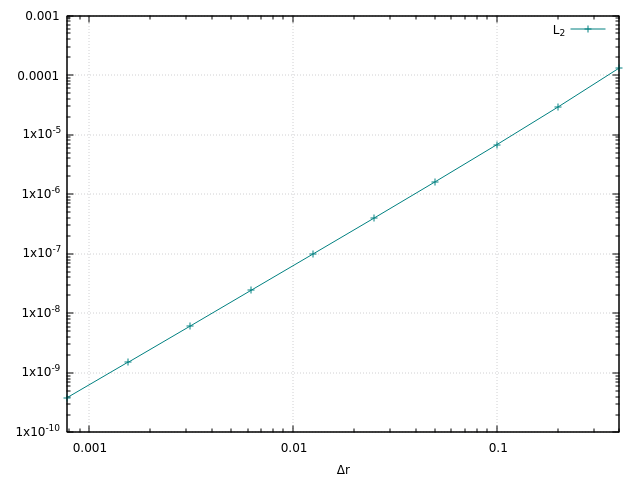
\includegraphics[width=\textwidth]{Figures/l2vDr}
% \end{figure}


% \begin{figure}[h]
%     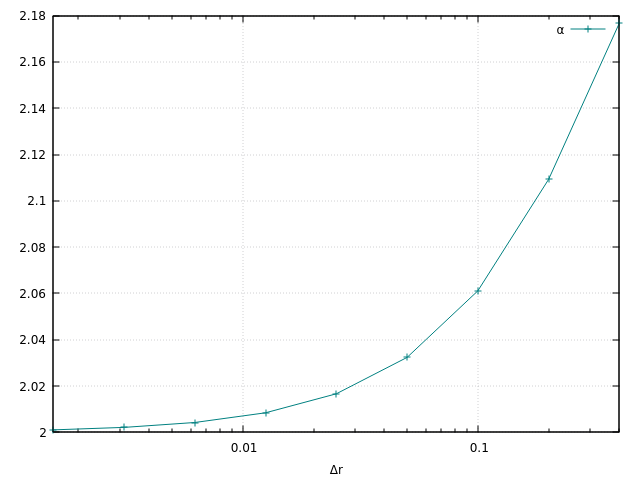
\includegraphics[width=\textwidth]{Figures/alphaVdr}
% \end{figure}


\section{Conclusion}
\section{Appendix}

\subsection{Error Analysis}


Reference: A. Ralston, A first course in numerical analysis 2nd edition

\subsubsection{Exact Polynomial Approximation}


Say we have some discrete data,

\begin{equation*}
    \left( x_{i},y_2 \right),\left( x_2, y_2 \right), \dots , \left( x_n,y_n \right)
\end{equation*}
We want to find a polynomial of the LEAST degree that gits these points exactly. 
Such a polynomial is called a Lagrange Polynomial. If in addition you supply a
function, or derivative value, you can use Hermitie intepolation to help the 
desired fitted polynomial handle sudden changes (?)

For Lagrange Polynomials, the general form is,

\begin{equation*}
    p\left( x_i  \right) =
    \sum_{j=1}^{n} l_j(x_i) f(x_j) + \underbrace{\frac{f^{(n)}\left( c \right)}
    {n!}p_n(x_i)}_{\text{Error at } x_i},
\end{equation*}
where,

\begin{equation*}
    p_n(x_i) = \prod_{j = 1}^{n} \left( x_i - x_j \right) 
\end{equation*}

\begin{equation*}
    p_n(x_i) =  \left( x_{i} - x_{j} \right) 
    \left( x_i - x_{i+1} \right)
    \left( x_i - x_{i+2} \right)
    \left( x_i - x_{i+3} \right) \dots
    ( x_i - x_n)
\end{equation*}

So if we have two data points $x_i$ and $x_{i+1}$, the function of least degree
that fits the data \textit{exactly} for a Langrange interpolation is,

\begin{equation*}
    p(x_i) = l_{i}(x_i)f(x_{i}) + l_{i+1}(x_{i+1})f(x_{i+1}) + \left[\text{
        Error at $x_i$}
    \right]
\end{equation*}

Note that I said \textit{exactly}! So I will drop the error term\dots

Then we \textit{claim} that

\begin{align*}
    p(x_i) =  
    l_i\left( x_i\right)f_i\left( x_i\right) + 
    l_{i+1}\left( x_{i+1}\right)f_{i+1}\left( x_{i+1}\right) 
\end{align*}

which means that we also claim that
\begin{align*}
    l_i(x) = \frac{x - x_{i+1}}{x_{i} - x_{i+1}} \\
    l_{i+1}(x) = \frac{x - x_{i}}{x_{i+1} - x_{i}}
\end{align*}

if $x = x_i$,
\[ l_i(x_i) = \frac{x_i - x_{i+1}}{x_i - x_{i+1} }= 1\], 
\[l_{i + 1}(x_i) = \frac{x_i-x_i}{x_{i+1} - x_{i}} = 0\]
and 
if $x = x_{i+1}$,

\[ l_i(x_{i+1}) = \frac{x_{i+1} - x_{i+1}}{x_i - x_{i+1} }= 0\], 
\[l_{i + 1}(x_{i+1}) = \frac{x_{i+1}-x_i}{x_{i+1} - x_{i}} = 1\]

let's see if $p\left( x \right)$ passes through these points exactly,

\begin{align*}
    p\left( x_i \right) &= 1 f_i(x_i) + 0 f\left( x_i  \right) =  f\left( x_i  \right) \\
    p\left( x_{i+1} \right) &= 1 f_{i+1}(x_{i+1}) + 0 f\left( x_{i+1}  \right) =  f\left( x_{i+1}  \right) 
\end{align*}

Defining,

\begin{align*}
    \Delta x^+ &= x_{i+1} - x_i \\
    \hat{x} &= x - x_i 
\end{align*}
Using this on the Lagrange polynomial for two points gives 

\begin{align*}
    \left( \frac{
            \left( x - x_{i+1} \right)
            }{
            \left( x_i - x_{i+1} \right)
        }
        f_i
        + \frac{
            \left( x - x_i  \right)
            }{
            \left(x_{i+1}- x_i \right)
        }
        f_{i+1}
    \right) \\
    \left( 
        \frac{
            \left( x - \left( x_{i+1} \right) \right)
            }{
            \left( x_i - x_{i+1}\right)
        } 
        f_i + 
        \frac{
            \left( x + \left( -x_i \right) \right)
            }{
            \left( \left( x_{i+1} \right) + \left( -x_i \right) \right)
        }
        f_{i+1}
    \right) \\
    \left(
        \frac{
            (x-\left( \Delta x^+ + x_i \right)) 
            }{
            x_i - (\Delta x^+ + x_i)
        }
        f_i
        +
        \frac{ 
            \left( x + \left( \hat{x} - x \right) \right)
            }{
            \left( \left( \Delta x^+ + x_i \right) + \left( -x_i \right) \right)
        }
        f_{i+1}
    \right)  \\
    \left(
        \frac{
            (\left(x-x_i  \right) -\Delta x^+)   
            }{ 
            - \Delta x^+ 
        }
        f_i
        +
        \frac{
            \left(   \hat{x}    \right)
            }{\left( \left(  \Delta x^+ + x_i \right)  + \left( -x_i \right) \right)
        } f_{i+1}
    \right) \\
    \frac{
        \hat{x} - \Delta x^+
        }{
        -\Delta x^+
    }
    f_i
    +
    \frac{
        \hat{x}
        }{
        \Delta x^+
    }
    f_{i+1}
\end{align*}

The Lagrange polynomial is

\begin{equation*}
    \widetilde{f}\left( \hat{x} \right) 
    =
    \left( 
        \frac{\hat{x}}{\Delta x^+}f_{i+1} +
        \frac{\Delta x^+ - \hat{x}}{\Delta x^+}f_i
    \right)
\end{equation*}

\subsection{Integration}

Recall that 

\[ \hat{x} = x - x_i\]
Now we prepare to integrate,

\begin{align*}
    \int_{x_1}^{x_2} \widetilde{f} dx &=
    \int_{x_1-x_i}^{x_2-x_i} \widetilde{f} \frac{\partial x}{\partial \hat{x}}d\hat{x}\\
                                      &=
                                      \int_{x_1-x_i}^{x_2 - x_i} \widetilde{f} d\hat{x}
\end{align*}

In the interior of the domain $i = 1, iMax - 1$, the function is integrated 
from $\hat{x} = 0$ to $\hat{x} = \Delta x^+$. In other words ,the integration 
covers the complete range of the polynomial. Note that we are only integrating
over a single interval.

\begin{align*}
    \int_0^{\Delta x^+} \widetilde{f} d\hat{x}&=
    \int_0^{\Delta x^+}
    \left( 
        \frac{\hat{x}}{\Delta x^+}f_{i+1} +
        \frac{\Delta x^+ - \hat{x}}{\Delta x^+}f_i
\right) \\ &= 
\frac{1}{\Delta x^+}f_{i+1}
\int_{0}^{\Delta x^+} 
\left(\hat{x}  \right) d\hat{x}
+
\frac{1}{\Delta x^+}
f_{i}
\left(
    \int_{0}^{\Delta x^+} 
    \left( \Delta x^+  \right) d\hat{x}
    -
    \int_{0}^{\Delta x^+} 
    \left( 
        \hat{x}
    \right) d\hat{x}
\right)\\
           &=\frac{1}{\Delta x^+}
           \left( 
               f_{i+1}\left[ 
                   \frac{\left( \Delta x^+ \right)^2}{
                   2} - 0
               \right]_0^{\Delta x^+}
               +
               f_i
               \left[ 
\frac{\left( \Delta x^+ \right)^2}{
                   2} - 0
               \right]_0^{\Delta x^+}
           \right) \\ &=
           \frac{\left( \Delta x^+ \right)^2}{2 \Delta x^+}
           \left[ f_{i+1} +f_i\right] \\
           &= 
           \frac{\Delta x^+}{2 }
           \left[ f_{i+1} +f_i\right] 
\end{align*}
Which is the trapezoidal rule!
\subsection{Taylor Series Error Analysis}

Here we try to determine the order of accuracy of the trapezoidal rule. 
The Taylor series for the integral $F$ and for the function $f$ are:

\begin{align*}
    f_{i+1} &= f_i +
    \Delta x \frac{\partial f}{\partial x}|_i +
    \frac{\Delta x^2}{2} \frac{\partial^2 f}{\partial x^2}|_i +
    \mathcal{O}\left( \Delta x^3 \right) \\
    f_i &= f_i
\end{align*}
Summing the two gives,

\begin{align*}
f_i + f_{i+1} = 2 f_i  + \Delta x \frac{\partial f}{\partial x } +
\mathcal{O}\left( \Delta x^2 \right) 
\end{align*}
Multiplying by $\Delta x /2  $

\begin{align*}
    \frac{\Delta x}{2 }(f_i + f_{i+1} )= 
    f_i {\Delta x} + \frac{\Delta x ^2}{2}\frac{\partial f}{\partial x } +
\mathcal{O}\left( \Delta x^3 \right) 
\end{align*}


\subsection{Composie Trapezoidal Rule}
To account for the entire domain, we express our trapezoidal rule as the sum 
of sub intervals for a uniform grid, to do so we redefine the grid spacing,

\[\Delta x^+   = \frac{\Delta \widetilde{ x}^+  }{n - 1}   \]

where $\widetilde{x}+$ is the length of the domain
and $n$ is the total number of grid points. 

\begin{align*}
    \int_{x_1}^{x_n} \widetilde{f} d \hat{x} &= 
    \frac{\Delta x^+}{2} \sum_{i=1}^{n}
    \left( 
        f_i + f_{i+1}
    \right) \\ 
    &=
    \frac{\Delta x^+}{2}  
    \left[ 
        \left( f_1 + f_2 \right) +
        \left( f_2 + f_3 \right)  +\dots +
        \left( f_{n-2} + f_{n-1} \right) + 
        \left( f_{n-1} + f_{n} \right)  
    \right] \\
    &=
    \frac{\Delta x^+}{2}  
    \left[ 
        \left( f_1 +
            2f_2  +
         2f_3+\dots +
         2f_{n-2} + 
         2f_{n-1}  + 
         f_{n} \right)  
    \right] \\
    &=
    \frac{\Delta x^+}{2}
    \left[ 
        f_1 + f_n + 
        2 \sum_{i=2}^{n-1}
        f_i
    \right] \\
    &=
    \frac{\Delta x^+}{2}
    \left[ 
        f_1 + f_n \right] 
        + 
        \Delta x^+ \sum_{i=2}^{n-1}
    f_i
\end{align*}

Noe we can use A taylor series expansion on the composite trapezoidal rule to
get an order of accuracy

the summation will be expanded Around $ i \Delta x$ in order to interpret the sum 
as a Riemann sum
\begin{align*}
    f_1  &= f_1\\
    i\Delta x \frac{\partial f }{\partial x } +
    \frac{(i\Delta x)^2}{2!} \frac{\partial^2 f }{\partial x^2 } +
    \frac{(i\Delta x)^3}{3!} \frac{\partial^3 f }{\partial x^3 } + \dots
\end{align*}

Let's further simplify the Taylor series at the last grid point,
\begin{align*} 
    f_n &= f_1 + 
    \Delta \widetilde{x}^+\frac{\partial f }{\partial x  } +
    \frac{(\Delta \widetilde{x}^+)^2}{2!}\frac{\partial^2 f }{\partial x^2  } +
    \frac{(\Delta \widetilde{x}^+)^3}{3!}\frac{\partial^3 f }{\partial x^3  } + \dots \\
        &= 
        f_1 +
        \left( n - 1 \right)\Delta x^+ 
        \frac{\partial f}{\partial x} +
        \frac{\left( n - 1 \right)^2}{2}\Delta x^+ 
        \frac{\partial^2 f}{\partial x^2} +
        \frac{\left( n - 1 \right)^3}{3}\Delta x^+ 
        \frac{\partial^3 f}{\partial x^3}
\end{align*}

Okay this is a bit tricky, lets distribute the summation on the Taylor series 
expanded around each grid point. Since this Taylor Series expanison involves 
the 1st grid point we re-adjust our summation to show this.

\begin{align*}
    \sum_{i = 2}^{n - 1} f_i  &= 
    \sum_{i = 1}^{n - 2} \left( 
    f_1 +
    i\Delta x \frac{\partial f }{\partial x } +
    \frac{(i\Delta x)^2}{2!} \frac{\partial^2 f }{\partial x^2 } +
    \frac{(i\Delta x)^3}{3!} \frac{\partial^3 f }{\partial x^3 } + \dots
    \right) \\
                              &=
    \sum_{i = 1}^{n - 2} \left( 
    f_1 \right) +
    \sum_{i = 1}^{n - 2} \left( 
    i\Delta x \frac{\partial f }{\partial x }\right) +
    \sum_{i = 1}^{n - 2} \left( 
    \frac{(i\Delta x)^2}{2!} \frac{\partial^2 f }{\partial x^2 } \right)+
    \sum_{i = 1}^{n - 2} \left( 
    \frac{(i\Delta x)^3}{3!} \frac{\partial^3 f }{\partial x^3 } \right)+ \dots\\ 
                              &=
    \sum_{i = 1}^{n - 2} \left( 
    f_1 \right) +
 \Delta x \frac{\partial f }{\partial x }   
     \sum_{i = 1}^{n - 2} \left( i\right) +
    \frac{(\Delta x)^2}{2!} \frac{\partial^2 f }{\partial x^2 } 
    \sum_{i = 1}^{n - 2} \left( i^2 \right)
    +
    \frac{(\Delta x)^3}{3!} \frac{\partial^3 f }{\partial x^3 } 
    \sum_{i = 1}^{n - 2} \left( i^3 \right)
\end{align*} 
Now we can  substitute this into the composite trapezoial rule and gather the coefficients 


\begin{align*}
    \frac{\Delta x^+ }{2}\left[ f_1 + f_n \right] + \Delta x^+ \sum_{i=1}^{n-2} f_i 
\end{align*}
Let's look at one common term at a time, starting with $f_1$, note the two halfs
summing to one,
\begin{align*} \frac{\Delta x^+}{2}\left[ f_1 + f_1 + \sum_{i=1}^{n-2} f_1 \right] \\
    \Delta x^+ f_1\left[ 1 + \sum_{i=1}^{n-2}1 \right]
\end{align*}

Now for the rest of the terms, we factor out $\Delta x^+$
\begin{align*}
    (\Delta x^+)^2 \frac{\partial f}{\partial x } \left(
        \sum_{i = 1}^{n - 2} \left( i\right) + \frac{n-1}{2} \right) + \\
        \frac{(\Delta x^+)^3}{2!} \frac{\partial^2 f}{\partial x^2 } \left(
    \sum_{i = 1}^{n - 2} \left( i\right)^2 + \frac{(n-1)^2}{2} \right)  + \\
    \frac{(\Delta x^+)^4}{3!} \frac{\partial^3 f}{\partial x^3 } \left(
    \sum_{i = 1}^{n - 2} \left( i\right)^3 + \frac{(n-1)^3}{2} \right) \dots
\end{align*}

Using the following summation rules we can further simplify the problem


\begin{align*}
    \sum_{i = 1}^{n}c= cn  \\
    \sum_{i = 1}^{n}i =  \frac{n\left( n-1\right)}{2}  \\
    \sum_{i = 1}^{n}i^2  = \frac{n^3}{3} + \frac{n^2}{2} + \frac{n}{6}   \\
    \sum_{i = 1}^{n}i^3  = \frac{n^4}{4} + \frac{n^3}{2} + \frac{n^2}{4}  
\end{align*}
Let's put the terms back together, and then simplify with the closed form 
expressions for the summations,
\begin{align*}
    \Delta x^+ f_1\left[ 1 + \sum_{i=1}^{n-2}1 \right] + \\
    (\Delta x^+)^2 \frac{\partial f}{\partial x } \left(
        \sum_{i = 1}^{n - 2} \left( i\right) + \frac{n-1}{2} \right) + \\
        \frac{(\Delta x^+)^3}{2!} \frac{\partial^2 f}{\partial x^2 } \left(
    \sum_{i = 1}^{n - 2} \left( i\right)^2 + \frac{(n-1)^2}{2} \right)  + \\
    \frac{(\Delta x^+)^4}{3!} \frac{\partial^3 f}{\partial x^3 } \left(
    \sum_{i = 1}^{n - 2} \left( i\right)^3 + \frac{(n-1)^3}{2} \right) \dots
\end{align*}

\begin{align*}
    \Delta x^+ f_1\left[ 1 + (n - 2)  \right] + \\
    (\Delta x^+)^2 \frac{\partial f}{\partial x } \left(
    \frac{(n-2)[\left( n-2 \right)-1]}{2} + \frac{n-1}{2} \right) + \\
        \frac{(\Delta x^+)^3}{2!} \frac{\partial^2 f}{\partial x^2 } \left(
        \frac{(n-2)^3}{3} + \frac{(n-2)^2}{2} + \frac{(n-2)}{6} + \frac{(n-1)^2}{2} \right)  + \\
    \frac{(\Delta x^+)^4}{3!} \frac{\partial^3 f}{\partial x^3 } \left(
    \frac{(n-2)^4}{4} + \frac{(n-2)^3}{2} + \frac{(n-2)^2}{4} + \frac{(n-1)^3}{2} \right) \dots
\end{align*}

\begin{align*}
    \Delta x^+ f_1\left[ (n - 1)  \right] + \\
    (\Delta x^+)^2 \frac{\partial f}{\partial x } \left(
    \frac{(n-2)\left( n-1 \right)}{2} + \frac{n-1}{2} \right) + \\
        \frac{(\Delta x^+)^3}{2!} \frac{\partial^2 f}{\partial x^2 } \left(
        \frac{(n-2)^3}{3} + \frac{(n-2)^2}{2} + \frac{(n-2)}{6} + \frac{(n-1)^2}{2} \right)  + \\
    \frac{(\Delta x^+)^4}{3!} \frac{\partial^3 f}{\partial x^3 } \left(
    \frac{(n-2)^4}{4} + \frac{(n-2)^3}{2} + \frac{(n-2)^2}{4} + \frac{(n-1)^3}{2} \right) \dots
\end{align*}

\begin{align*}
     f_1\left[ \Delta \widetilde{x}^+  \right] + \\
    (\Delta x^+)^2 \frac{\partial f}{\partial x } \left(
    \frac{(n-2)\left( n-1 \right)}{2} + \frac{n-1}{2} \right) + \\
        \frac{(\Delta x^+)^3}{2!} \frac{\partial^2 f}{\partial x^2 } \left(
        \frac{(n-2)^3}{3} + \frac{(n-2)^2}{2} + \frac{(n-2)}{6} + \frac{(n-1)^2}{2} \right)  + 
\end{align*}

Side note: 

\begin{align*}
    \frac{(n - 2)(n-1)}{2} + \frac{(n-1)}{2}\\
    \frac{(n - 2)(n-1) + (n-1)}{2} 
\end{align*}
Factor out $(n-1)$
\begin{align*}
    \frac{\left[ \left( n - 2 \right) + 1 \left( n - 1 \right) \right]}{2} \\
    \frac{\left( n-1 \right)\left( n - 1 \right)}{2} \\
    \frac{\left( n - 1 \right)^2}{2}
\end{align*}

Using this for the coefficient of the second term,

\begin{align*}
     f_1\left[ \Delta \widetilde{x}^+  \right] + \\
    (\Delta x^+)^2 \frac{\partial f}{\partial x } \left(
    \frac{(n-1)^2}{2}  \right) + \\
        \frac{(\Delta x^+)^3}{2!} \frac{\partial^2 f}{\partial x^2 } \left(
        \frac{(n-2)^3}{3} + \frac{(n-2)^2}{2} + \frac{(n-2)}{6} + \frac{(n-1)^2}{2} \right)  +
\end{align*}

Since we expect the third term to have a $\left( n-1 \right)^3$ if this pattern
of the Taylor series being expanded around L, the coefficient of the third term
is going to be set equal to $\left( n-1 \right)^3$ and simplified,

We also expect the leading coeffient to have 1/6 as well. Multiplying by 3
and setting the result equal $(n-1)^3$ gives,
\begin{align*}
    \left(
    (n-2)^3 + \frac{3(n-2)^2}{2} + \frac{(n-2)}{3} + (n-1)^2 
    \right)
    &=
    (n-1)^3 \\
    \frac{n-1}{2}
\end{align*}
Plugging this back in, along with the definition of $\Delta \widetilde{x}^+$ for
the rest of the terms gives,


\begin{align*}
     f_1\left[ \Delta \widetilde{x}^+  \right] + \\
 \frac{(\Delta \widetilde{x}^+)^2}{2}     \frac{\partial f}{\partial x }  + \\
 \frac{(\Delta x)^3}{3!} \frac{\partial^2 f}{\partial x^2 } 
 \frac{ \Delta \widetilde{x}^+
 }{2\Delta x}
 \end{align*}






\end{document}
